\documentclass{article}
\usepackage[utf8]{inputenc}
\usepackage[T1]{fontenc} 
\usepackage[french]{babel}

\usepackage{appendix}
\usepackage{pdfpages}

\usepackage{hyperref}
\usepackage[top=2.5cm, bottom=2.5cm, left=2.5cm, right=2.5cm]{geometry}
\usepackage{setspace}

\usepackage{graphicx}
\usepackage{fancyhdr}
\usepackage{xcolor}

\graphicspath{{img/}}

\hypersetup{
    colorlinks=true,
    urlcolor=brown,
    linkcolor=blue,
    breaklinks=true
}

\begin{document}
\onehalfspacing

\begin{titlepage}
    \vspace{2cm}
    \centerline{\rule{13cm}{0.6pt}}
    \vspace{0,65cm}
    \centering
    {\Huge \textbf{Application interactive de colorisation d'images par deep learning}}\par
    \vspace{0,65cm}
    \centerline{\rule{13cm}{0.6pt}}
    \vspace{0.5cm}
    {\Huge \textbf{Cahier des charges} }\par
    \vspace{0.5cm}
    \centerline{\rule{13cm}{0.6pt}}
    \vspace{0.5cm}
    {\Huge Adrien Aguila--Multner }\par
    \vspace{0.25cm}
    {\Huge Ismail Alouani }\par
    \vspace{0.25cm}
    {\Huge Mohamed Bahloul }\par
    \vspace{0.25cm}
    {\Huge Ahmed Bahri }\par
    \vspace{0.25cm}
    {\Huge Ilyes Cheikh}\par
    \vspace{0.25cm}
    {\Huge Cléa Rebillard}\par
    \vspace{0.25cm}
    {\Huge Priscilla Tissot}\par
    \vspace{0.25cm}
    {\Huge Simon Villechenaud}\par
    \vspace{1.5cm}
    \begin{center}
    
\includegraphics[height=4cm]{logo_em.jpeg}
    \end{center}
    \vspace{1.5cm}
     \begin{minipage}{0.4\textwidth}
      \begin{flushleft} \large
        2022-2023\\
        Deuxième année\\
      \end{flushleft}
    \end{minipage}
    \begin{minipage}{0.4\textwidth}
      \begin{flushright} \large
        Filière Informatique\\
        Encadrant : M. Ta\\
        Client : M. Clément
      \end{flushright}
    \end{minipage}
    \vspace{4cm}
    %\includegraphics[height=4.5cm]{logo.png}
    \thispagestyle{empty}
\end{titlepage}

\pagebreak

\tableofcontents

\pagebreak


\section{Introduction}

La colorisation d'image est un processus qui ajoute des couleurs à une image ou une vidéo originalement en niveaux de gris.
L'objectif est d'avoir des couleurs à la fois réalistes et plaisantes au regard. 
Cela est notamment utilisé sur des images ou films d'archive afin d'avoir une représentation plus visuelle de ces scènes.
Ce projet a pour but de fournir des méthodes guidées par l’utilisateur afin de faire de la
colorisation d’images. Cela s'inscrit dans le cadre du projet de recherche PostProdLEAP qui vise à éditer des images d'archive 
avec l'entreprise Composite Films pour faire de la colorisation de films historique. 

Les méthodes actuelles donnant les meilleurs résultats sont des programmes utilisant le \emph{deep-learning}.
Il s'agit d'un champ de l'apprentissage automatique se basant sur des réseaux de neurones artificiels entraînés sur de larges banques de données.

Ces méthodes sont diverses mais l'on peut distinguer 2 catégories principales :
d'abord les méthodes entièrement automatiques, proposées pour la première fois par Cheng \emph{et al} \cite{journals/corr/ChengYS16}, qui peuvent coloriser une image sans aucun apport additionnel. 
Elles souffrent cependant d'un manque de couleurs vives et réalistes. De plus elles sont souvent biaisées par les données sur lesquelles elles sont entraînées.

Ensuite, d'autres méthodes prennent en compte l'entrée d'un utilisateur : soit des \emph{scribbles}, des points ou traits de couleurs donnés par l’utilisateur sur l’image
en noir et blanc, comme proposé par Levin \emph{et al}. \cite{10.1145/1015706.1015780}, soit des images de référence dont on utilise les couleurs comme étudié par Irony \emph{et al.} \cite{10.5555/2383654.2383683}.
Cela permet d'avoir des couleurs réalistes et conformes à ce que veut l'utilisateur ; cependant cette technique nécessite de donner ces informations manuellement à chaque image. Cela peut se révéler coûteux en temps, bien que certains algorithmes permettent de choisir ces données automatiquement, comme par exemple Kim \emph{et al}., 2021 \cite{color-Bleeding}.

Un autre problème majeur de la colorisation est l'évaluation des résultats :
il existe des métriques quantitatives calculant la qualité d'une colorisation, mais elles ne sont pas toujours représentatives de la perception humaine, du respect de la sémantique ou de la structure de l'image.
Le but étant d'obtenir des images visuellement plaisantes et plausibles à l'oeil, la meilleure manière de savoir si une colorisation est bonne reste le jugement humain. Encore une fois, cela demande beaucoup de temps sur de nombreuses images.

L'objectif de ce projet est donc de fournir une application simplifiant l'utilisation de toutes ces méthodes, y compris l'ajout de \emph{scribbles} et le choix de références depuis une unique interface.
Celle-ci servira en même temps à visualiser les résultats obtenus et à les comparer.
Elle permettra aussi de faire évaluer les résultats de colorisation par des humains via des questionnaires personnalisables.

Ce document décrit les besoins et les objectifs du projet, les fonctionnalités attendues, les
contraintes et choix techniques, et les modalités de réalisation. Il est divisé en plusieurs sections. D'abord, la présentation générale du
projet, qui donne son contexte, son objectif global et les principaux acteurs impliqués. 
Ensuite, les exigences fonctionnelles qui détaillent un ensemble de fonctionnalités que le système doit être capable de faire.
Ces exigences sont décrites sous forme de scénarios d'utilisation, qui explicitent comment les utilisateurs interagiront avec le système.
Puis l'architecture technique du projet envisagée pour répondre aux différents problèmes sera présentée en détails.
Nous aborderons aussi la manière dont sera organisée et suivie la réalisation du projet : les tâches à effectuer, les ressources nécessaires, les délais et finalement les modalités de livraison.
\pagebreak

\section{Présentation du client}
Le client pour ce projet est M. Michaël Clément, maître de conférences à Bordeaux INP dans l'école d'ingénieurs ENSEIRB-MATMECA et chercheur en informatique au sein du Laboratoire Bordelais de Recherche en Informatique (LaBRI). 
Plus précisément, il fait partie du département image et son qui se consacre à des recherches sur l'acquisition, le traitement, l'analyse, la modélisation, la synthèse et l'interaction des médias audiovisuels.
Leur champ de recherche couvre tout le processus allant de la collecte de données à l'extraction d'informations ou à la restitution de données numériques.\\

Notre PFA (Projet au Fil de l'Année) s’inscrit dans le cadre d’un projet de recherche, \href{https://www.labri.fr/perso/bugeau/PostProdLEAP/}{PostProdLEAP}, mené par le LaBRI en collaboration avec des artistes et historiens de l’entreprise Composite Films. Composite Films est une entreprise française 
qui a pour objectif de restaurer d'anciennes images et films d'archive en leur ajoutant de la couleur. C'est un projet financé par l’Agence Nationale de la Recherche (ANR). L'objectif de PostProdLEAP est donc de développer de nouveaux outils pour l'édition d'images et de vidéos d'archives. Le projet vise plus spécifiquement à développer des moyens de coloriser des images en utilisant du \textit{deep-learning}, dans le but de simplifier le travail des historiens et artistes de Composite Films en leur proposant des outils qui requièrent moins de temps et sont plus faciles à utiliser. Il s'agit aussi de développer de nouvelles méthodes qui permettent de régler les problèmes rencontrés avec les techniques actuelles.
En effet, les méthodes de colorisation existantes ont plusieurs limites, comme par exemple le débordement de couleurs sur des objets voisins ou encore un manque de détails. Certaines de ces méthodes ne sont donc pas adaptées à la colorisation d'archives anciennes car le résultat peut ne pas paraître réaliste. PostProdLEAP cherche à trouver des solutions à ces problématiques, et notre projet a pour but de les aider dans leur travail.


\section{Le projet : application interactive de colorisation d'images par deep learning}

Dans cette section, nous allons décrire le sujet et la démarche que nous avons adopté afin de mieux le comprendre et de
créer les bases du projet. 
Nous allons également détailler les besoins fonctionnels ainsi que le socle architectural que nous proposons afin de 
répondre à ces exigences.

\subsection{Description du sujet}

Ce projet concerne la création d'une application pour la colorisation d'images avec des méthodes utilisant des réseaux de neurones convolutifs.
L'application servirait à coloriser des images de manière automatique en utilisant les différentes méthodes qui existent. L'interface à développer s'adresse principalement à des chercheurs du domaine qui souhaitent évaluer et comparer ces méthodes.
Ce projet s'oriente donc autour de trois points clés.
\\

Tout d'abord, le premier point relève de l'exécution des méthodes de colorisation.
Comme dit précédemment, la plupart des techniques de colorisation développées sont basées sur l’apprentissage supervisé avec l’utilisation de réseaux de neurones convolutifs (CNN). Ce sont des 
réseaux neuronaux dont l'architecture s'inspire du cortex visuel des animaux. Ces méthodes sont donc particulièrement utilisées dans la recherche concernant la colorisation d'images.
Il s'agit de s'intéresser à 3 de ces techniques en particulier : la colorisation par \textit{scribbles} où l’utilisateur renseigne des pixels de couleurs qui vont servir à augmenter la probabilité de l’utilisation de cette couleur dans l’espace indiqué, 
la colorisation par référence où l’utilisateur indique une image référence pour que le modèle utilise la même palette de couleurs et 
la colorisation automatique qui se fait sans aucun apport additionnel.
L'application devra donc permettre à l'utilisateur (ici le chercheur) d'exécuter plusieurs méthodes qui suivent ces techniques, sur des images qu'il aura choisi.
Elle devra être interactive en permettant aux utilisateurs de renseigner certaines données comme des \textit{scribbles} ou des images de référence
s'ils choisissent des méthodes qui en nécessitent.
%L’application devra permettre l’utilisateur de choisir entre ses trois méthodes de coloration ainsi que choisir le modèle à appliquer.
\\

Le deuxième aspect de se projet concerne la visualisation des images et, en particulier, la visualisation des résultats des colorisations effectuées. 
L'application doit offrir la possibilité de visionner des colorisations d'une même image utilisant différentes méthodes afin de les comparer.
Il faut donc que l'interface puisse afficher des images côte à côte et permette de les observer finement avec différents outils, comme par exemple le zoom.
De plus, l’évaluation de l’image peut être faite automatiquement par des mesures quantitatives comme PSNR (\textit{Peak Signal to Noise Ratio}), LPIPS (\textit{Learned Perceptual Image Patch Similarity}) ou SSIM (\textit{Structural Similarity}) .Celles-ci permettent de comparer l’image en couleurs d'origine (\textit{groundtruth} ou vérité terrain) et l'image colorisée
en évaluant différents aspects. Ces mesures sont des indicateurs pour les chercheurs afin d'évaluer la qualité des colorisations.
Il faut donc que l'interface permette de les calculer et de les afficher avec les images.
% Mais l'œil humain reste le comparatif le plus précis. 
% Donc, l’application devra également permettre à l’utilisateur de visualiser les images traitées et de comparer des colorisations d’une même image par rapport aux différentes méthodes que ce soit qualitativement ou quantitativement.
\\

Outre les deux aspects mentionnés précédemment, la dernière fonctionnalité importante que l'application devra comporter est
un système de questionnaires permettant d’obtenir des données pour comparer les différentes méthodes. Ces questionnaires 
doivent permettre de recueillir les préférences qualitatives de multiples utilisateurs sur des colorisations de différentes images.
Ces préférences sont relatives aux impressions et aux opinions que les utilisateurs peuvent avoir quant à la qualité
des colorisations. Elles complètent des mesures quantitatives qui permettent de recueillir des mesures numériques sur les colorisations effectuées.
Les mesures quantitatives peuvent se calculer facilement en les implémentant informatiquement. Les questionnaires sont donc nécessaires
pour recueillir les préférences des utilisateurs et ainsi pouvoir évaluer les méthodes de colorisation de manière différente, 
en approfondissant les analyses pour en saisir les subtilités. Cette partie se distingue des deux autres parties car elle sera utilisée non seulement 
par des chercheurs du domaine mais aussi par des personnes qui sont extérieures.
\\

Ce projet vise donc à créer une application qui offre la possibilité d’appliquer des méthodes de colorisation, 
de comparer les images obtenues en utilisant une visionneuse d’images et d'évaluer qualitativement ces résultats en utilisant 
des questionnaires dédiés aux utilisateurs. \\

Le sujet explicité d'une telle manière est imprécis et n'est pas suffisant pour démarrer un projet. Afin de spécifier ce sujet
et les attentes du client, nous avons réalisé une analyse fonctionnelle que nous décrivons dans la partie suivante.

\subsection{Analyse des besoins fonctionnels}\label{sec:analyse-fonctionnelle}

Afin de cerner plus précisément les besoins du client, il faut effectuer une analyse fonctionnelle qui permet de comprendre
et de concevoir les fonctionnalités que l'application devra comporter. L'analyse fonctionnelle a été réalisée lors des réunions avec le client,
dans lesquelles nous avons discuté de ses exigences pour le projet. Dans le cadre d'une méthodologie agile, cette analyse est réalisée en ce plaçant du
point de vue de l'utilisateur. Pour cela, nous avons adopté une approche \textit{design first} que nous détaillons dans la section \ref{sec:design-first}. Il s'agit ainsi d'imaginer les interactions de l'utilisateur avec le système pour réaliser certains objectifs. 
Il est possible de réaliser l'analyse fonctionnelle à différents niveaux, afin d'imaginer 
des scénarios plus ou moins précis d'utilisation. On la sépare alors en deux niveaux de précision différents :
les \textit{use cases} et les \textit{user stories}.  Les \textit{user stories} offrent une perspective qui est strictement du point de vue de l'utilisateur et des différents scénarios d'utilisation qu'il sera amené à réaliser. 
Elles sont décrites en section \ref{sec:userstories}. Les \textit{use cases} visent à donner un aperçu 
des grandes fonctionnalités de l'application en détaillant le fonctionnement interne du système conjointement au comportement de l'utilisateur. Elles sont décrites en section \ref{sec:usecase}. 
Enfin, les \textit{user stories} ont été découpées en tâches, qui nous permettent de comprendre ce qui devra être réalisé pour les
compléter. Ces tâches sont explicitées dans la section \ref{sec:taches}.

\subsubsection{Une approche \textit{design first} par les maquettes}\label{sec:design-first}

Afin de définir les besoins du client, nous adoptons une démarche appelée \textit{design first}. Cette démarche est une approche qui permet de privilégier
le design au travers d'interfaces graphiques. Elle consiste à développer le design de l'application en premier, après avoir 
défini les besoins essentiels du client.
Elle s'oppose à une démarche \textit{code first} qui consiste à développer le code avant tout.
Cette méthode s'intègre bien dans une conception agile car elle permet de se placer du point de vue de l'utilisateur. En élaborant les interfaces avant tout,
nous imaginons les différents cas d'utilisation de l'application et la manière la plus pratique pour les utilisateurs d'utiliser les fonctionnalités désirées par le client.
Développer les interfaces tôt dans le projet a donc plusieurs avantages. Tout d'abord, cela permet de confirmer les besoins du client et de s'assurer au début du projet que 
toutes ses exigences ont bien été prises en compte. Une interface est un moyen simple et concret sur lequel le client est capable de se projeter, contrairement à 
une liste de besoins qui peut être difficile à analyser. L'interface permet à tous les acteurs (clients et équipe agile) de construire une application
en visualisant concrètement les scénarios d'utilisation (et les actions) qu'une personne pourra mener en s'en servant.
De plus, l'approche \textit{design first} permet à toutes les parties prenantes de discuter du projet avec un langage compris par tout le monde.
En effet, il peut parfois être difficile pour les développeurs et le client de se comprendre. L'équipe de développement peut employer des termes trop techniques et 
mentionner des mécanismes que le client peut ne pas comprendre. Le client quand à lui, aura souvent un langage propre à son domaine et à son métier, que les développeurs peuvent ne pas 
saisir dans son entièreté. Une interface graphique est donc une solution qui permet à tout le monde de communiquer clairement.

Pour ces raisons, cette approche \textit{design first} s'intègre bien dans ce projet. Nous avons donc choisi, une fois les besoins du client recueillis, de les représenter sous la forme 
de maquettes. Cela nous permet de rapidement remarquer des défauts dans les besoins que nous avons défini et de s'apercevoir si le client avait imaginé son application d'une manière différente.  
Dans les parties suivantes, nous décrivons les besoins fonctionnels que nous avons pu définir à l'aide de cette approche.

\subsubsection{Analyse des besoins utilisateur (\textit{user stories})} \label{sec:userstories}

Les \textit{user stories} permettent d'imaginer le point de vue d'un utilisateur lorsqu'il se sert de l'application. Dans les \textit{user stories}, sont renseignés : un utilisateur 
(en tant que), un objectif (je souhaite faire) et une raison pour cet objectif (pour que).
Ces \textit{user stories} figureront dans le \textit{backlog} qui répertorie tout ce qui sera à réaliser dans le projet.
Pour chacune d'entre elles, nous avons estimé une priorité (en fonction des besoins du client) ainsi qu'une estimation de temps 
qu'elle pourra prendre à être réalisée. Cette estimation de temps est importante car elle permet non seulement d'estimer la quantité de 
\textit{user stories} que nous serons capables de compléter dans le projet mais aussi d'estimer celles que nous pourrons faire lors 
d'une itération. Chacune des \textit{user stories} possède également un ou plusieurs critères d'acceptation, qui permettent de 
définir la condition pour qu'elle soit terminée. L'ensemble des \textit{user stories} se trouve en section \ref{sec:annexe-user-stories}. \\ 

Nous allons ici décrire les différents scénarios d'utilisation possibles du logiciel par un utilisateur.
On distinguera l'utilisateur du logiciel et l'utilisateur externe qui répond uniquement aux questionnaires.

Le produit doit en premier lieu permettre de coloriser des images.

En tant qu'utilisateur, je souhaite donc pouvoir importer depuis mon ordinateur une image ou un dossier d'images, au choix, afin de les coloriser.
Je souhaite ensuite pouvoir choisir une ou plusieurs méthodes de colorisation à appliquer parmi celles disponibles dans le logiciel.
Si l'une des méthodes requiert des scribbles, je souhaite avoir une interface qui permette d'en créer manuellement sur les images, puis de les enregistrer. 
Cette interface devrait me proposer une brosse de taille et couleur modifiable pour tracer les scribbles, une gomme pour les effacer et un bouton pour tous les effacer d'un coup.
Je veux qu'il soit aussi possible d'importer ces scribbles si je les ai déjà créé, et pouvoir alors les modifier de la même manière.
De même, si l'une des méthodes requiert des références, je souhaite pouvoir créer une configuration d'images de référence depuis l'interface, ou bien en importer une pré-existante sur mon disque.

Afin de mesurer la qualité des colorisations, j'aimerais pouvoir ajouter des métriques à calculer automatiquement sur les images résultats.
Ces métriques étant implémenté directement dans le logiciel, je veux pouvoir en ajouter de nouvelles simplement à la liste disponible pour ensuite les calculer lors de la colorisation.
De la même manière je souhaite avoir la possibilité d'ajouter des nouveaux modèles de colorisation à la liste présente dans le logiciel.

Enfin, je veux pouvoir lancer l'exécution de la colorisation avec toutes les images, méthodes avec leurs scribbles et références, et métriques sélectionnées, pour avoir les résultats générés sur mon disque.
\newline

L'application doit ensuite présenter une interface de visualisation des résultats obtenus.

En tant qu'utilisateur, je souhaite pouvoir charger un ou plusieurs dossiers d'images colorisées présents sur mon disque.
Je veux ensuite avoir accès à une interface présentant la liste des images chargées, dans laquelle je pourrai sélectionner une image ou la chercher par son nom.
Cela affichera alors les différentes colorisations associées, que je pourrai masquer si je n'en ai pas besoin.
Le but de cette interface sera de comparer les résultats; pour cela je veux pouvoir zoomer sur des zones précises de l'image en passant mon curseur dessus. Le zoom se fera sans interpolation pour ne pas biaiser la visualisation.
Il faudrait que le zoom puisse se faire au même endroit sur toutes les images simultanément pour avoir une bonne comparaison.
Enfin je veux que les métriques calculées soient affichées à côté des colorisations, mais que je puisse les masquer si besoin.
\newline

La dernière fonctionnalité de l'application est de permettre la réalisation et la réponse à des questionnaires.

Pour cela il faut qu'en tant qu'utilisateur je puisse créer des questions : d'abord en indiquant l'énoncé et le type de réponse attendu, c'est à dire tous les champs de réponse présentés à la personne interrogée.
Ensuite, je voudrais indiquer combien de colorisations seront montrées dans cette question. Il serait utile de pouvoir afficher des colorisations aléatoires parmi toutes celles d'une même image d'origine, mais en laissant la possibilité de toujours afficher l'image d'origine et/ou la vérité terrain.
Une fois ces informations renseignées, je veux pouvoir enregistrer la question.

Ces questions seront ensuite données dans un questionnaire : je souhaite donc pouvoir créer un questionnaire en lui donnant un nom.
Celui-ci concernera une liste d'images que je chargerai depuis mon disque. Je veux ensuite pouvoir appliquer une question précédemment créée à une image en particulier, ou à toutes les images à la fois.
Il serait bien de pouvoir rendre aléatoire l'ordre dans lequel les questions seront posées.

En tant qu'utilisateur externe, je souhaite ensuite pouvoir répondre au questionnaire ainsi créé.
Pour cela je souhaite pouvoir visualiser une question, les images associées, répondre aux questions dans les champs dédiés et passer à la suivante.
J'aimerais aussi pouvoir revenir à une question précédente si je change d'avis.

Une fois qu'assez d'utilisateurs externes ont répondu, je souhaite pouvoir visualiser ces réponses. Pour cela j'aimerais avoir une visualisation de chaque question, avec sur le même écran les réponses individuelles. 
J'aimerais aussi avoir des statistiques comme la moyenne ou la médiane sur les questions qui le permettent, afin d'analyser plus rapidement les réponses reçues.\\

Chacune de ces \textit{user stories} a une priorité. C'est un aspect essentiel car il nous permet de livrer en premier les fonctionnalités qui ont le plus de valeur pour le client.
Nous avons choisi de définir la priorité sur une échelle de 1 à 10, 10 étant le plus prioritaire.
Ainsi, plusieurs éléments peuvent être soulignés. Tout d'abord, nous avons défini, avec le client, que les parties d'exécution des colorisations et de visualisation
des résultats étaient plus prioritaires que les questionnaires. Dans ces parties, les différentes \textit{user stories} sont plus ou moins importantes.
De cette manière, nous avons déterminé que lors de la colorisation, le choix du répertoire d'image à coloriser était d'une priorité 10 alors que 
l'ajout de métrique à calculer lors de la colorisation était un peu moins prioritaire (priorité 4).
De même, pour la visualisation, avoir la possibilité de consulter la liste des images visualisable a une priorité maximale (c'est une des fonctionnalités essentielles du projet) tandis que pouvoir chercher une image parmi ces dernières
à l'aide d'une barre de recherche est bien moins prioritaire, avec une priorité de 2.
L'ensemble des priorités se trouve dans l'annexe \ref{sec:annexe-user-stories} contenant les \textit{user stories}.\\

Afin de compléter ces \textit{user stories}, il est nécessaire de créer des \textit{use cases}
afin de comprendre le fonctionnement du système lors de certaines actions des utilisateurs.

\subsubsection{Scénarios d'utilisation et interactions avec le système (\textit{use cases})} \label{sec:usecase}

Nous avons défini les \textit{use cases} conjointement aux \textit{user stories}. Un \textit{use case} correspond à une ou plusieurs \textit{user stories}. Les \textit{use cases} permettent donc de définir des actions qui seront faites avec l'application ainsi que le fonctionnement interne du système.
Ils concernent à la fois le client, qui pourra confirmer que les comportements imaginés de l'utilisateur sont corrects, et l'équipe de développement qui, grâce à eux, pourra commencer à envisager le fonctionnement de la solution.
Les cas d'utilisation que nous avons définis comportent :
\begin{itemize}
    \item Un \textbf{identifiant} pour les repérer facilement.
    \item Une \textbf{description} qui permet de comprendre l'action dont il s'agit.
    \item Une \textbf{liste de dépendances} afin de comprendre quel \textit{use case} devra être implémenté avant.
    \item Une \textbf{pré-condition} et une \textbf{post-condition} qui permettent respectivement de spécifier les conditions qui doivent être satisfaites avant et après l'action en question.
    \item Des \textbf{scénarios d'utilisation} qui spécifient les étapes qui seront réalisées à la fois par l'utilisateur et par le système lors de l'action. Ces scénarios peuvent être des scénarios d'utilisation normale, des scénarios alternatif ou encore des scénarios d'erreur.\\
\end{itemize}

L'ensemble des \textit{use cases} se trouve en section \ref{sec:annexe-use-case}. Nous pouvons détailler certains de ces \textit{use cases} afin de donner un aperçu de notre approche.
Le premier cas d'utilisation que nous allons décrire est le \textbf{paramétrage de la configuration de création et d'édition de scribbles}.
Cette fonctionnalité sera réalisée par une équipe de chercheurs. Elle ne comporte aucune dépendance (on imagine qu'on peut créer des \textit{scribbles} sans
vouloir exécuter une méthode juste après) et ne comporte aucune pré-condition. La condition à satisfaire une fois l'action réalisée est que
la configuration renseignée soit chargée sur l'interface de création/modification des scribbles.
Deux scénarios sont imaginés pour ce \textit{use case}. Ainsi le premier scénario imaginé est si l'utilisateur choisit de créer une nouvelle 
configuration de \textit{scribbles}. Il doit alors d'abord renseigner un nom pour la configuration dans le champs correspondant. Il doit ensuite
cliquer sur le champ qui permet de choisir le dossier des images concernées. Le système doit alors afficher une fenêtre surgissante
qui permet de choisir le répertoire voulu. L'utilisateur peut alors chercher le dossier qui l'intéresse et ensuite cliquer sur valider pour confirmer 
l'opération. Le système doit ensuite créer un nouveau dossier au bon emplacement avec le nom de la configuration et rediriger l'utilisateur
vers l'interface de création de \textit{scribbles}. Le scénario alternatif concerne le cas où les utilisateurs choisissent de charger une configuration
de \textit{scribbles} déjà créée. L'utilisateur clique alors sur le champ qui permet de choisir la configuration de \textit{scribbles}. Le système doit alors afficher 
l'interface qui permet de choisir un dossier. De même, l'utilisateur doit choisir le dossier et ensuite cliquer sur le bouton qui permet de charger les \textit{scribbles}.
Le système doit rediriger l'utilisateur vers l'interface qui permet de modifier les \textit{scribbles}.
Les figures \ref{fig:scenario-new-scribbles} et \ref{fig:scenario-load-scribbbles} résument les différents scénarios de cette fonctionnalité.\\

\begin{figure}[htp]
    \centering
    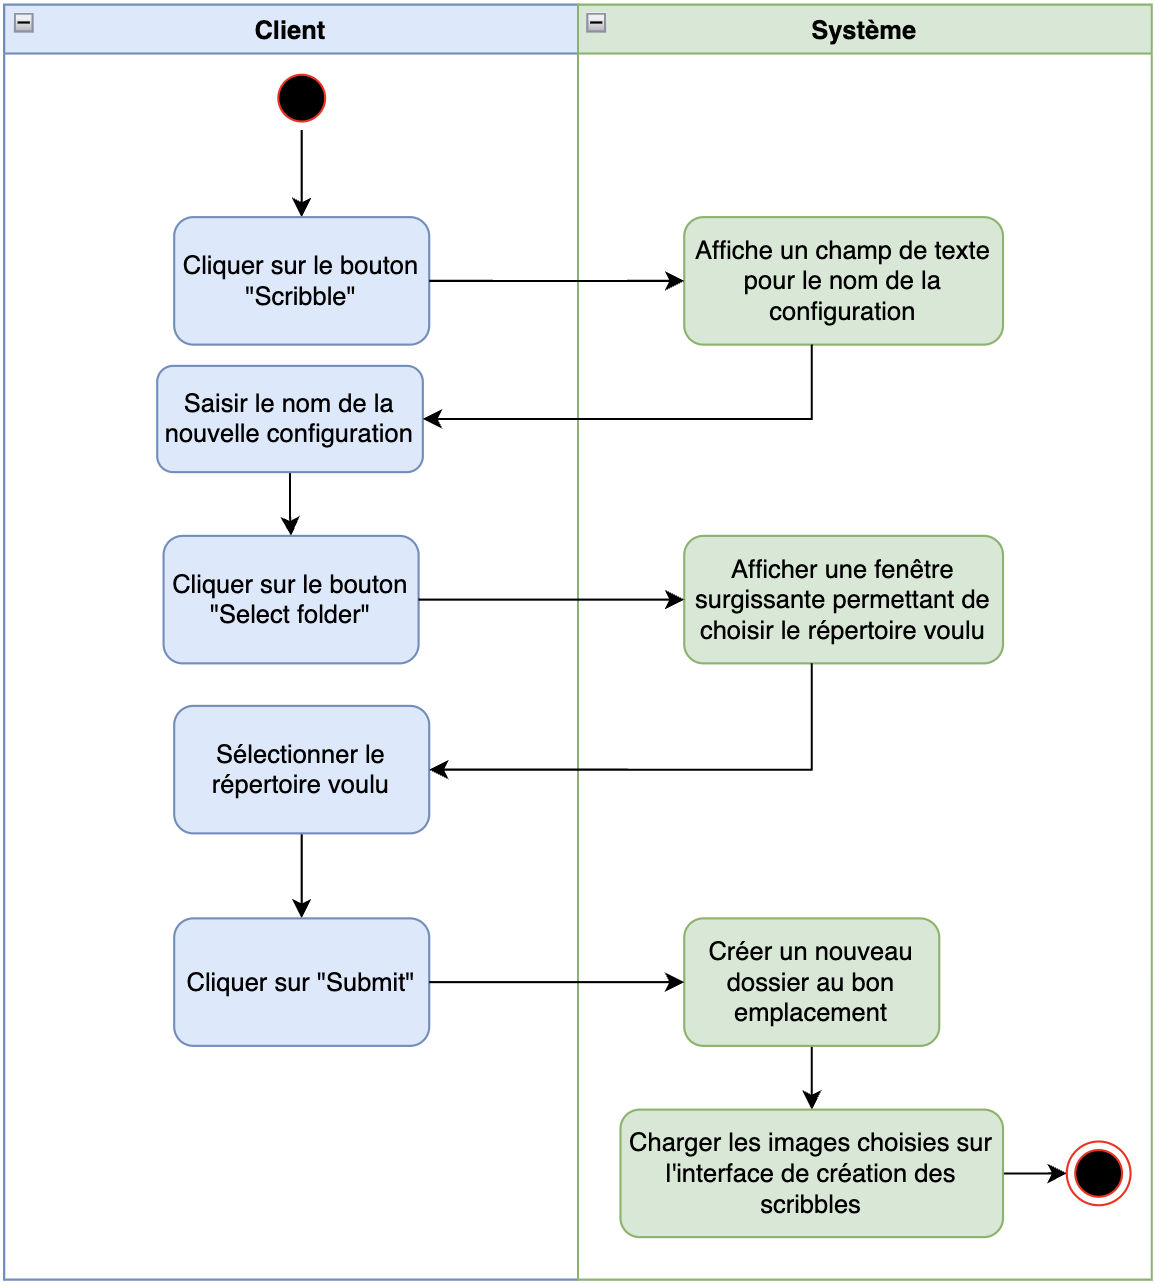
\includegraphics[width=10cm]{scenario-new-scribbles.png}
    \caption{Use case : Diagramme d'activité du scénario de création d'une configuration de scribbles}
    \label{fig:scenario-new-scribbles}
\end{figure}

\begin{figure}[htp]
    \centering
    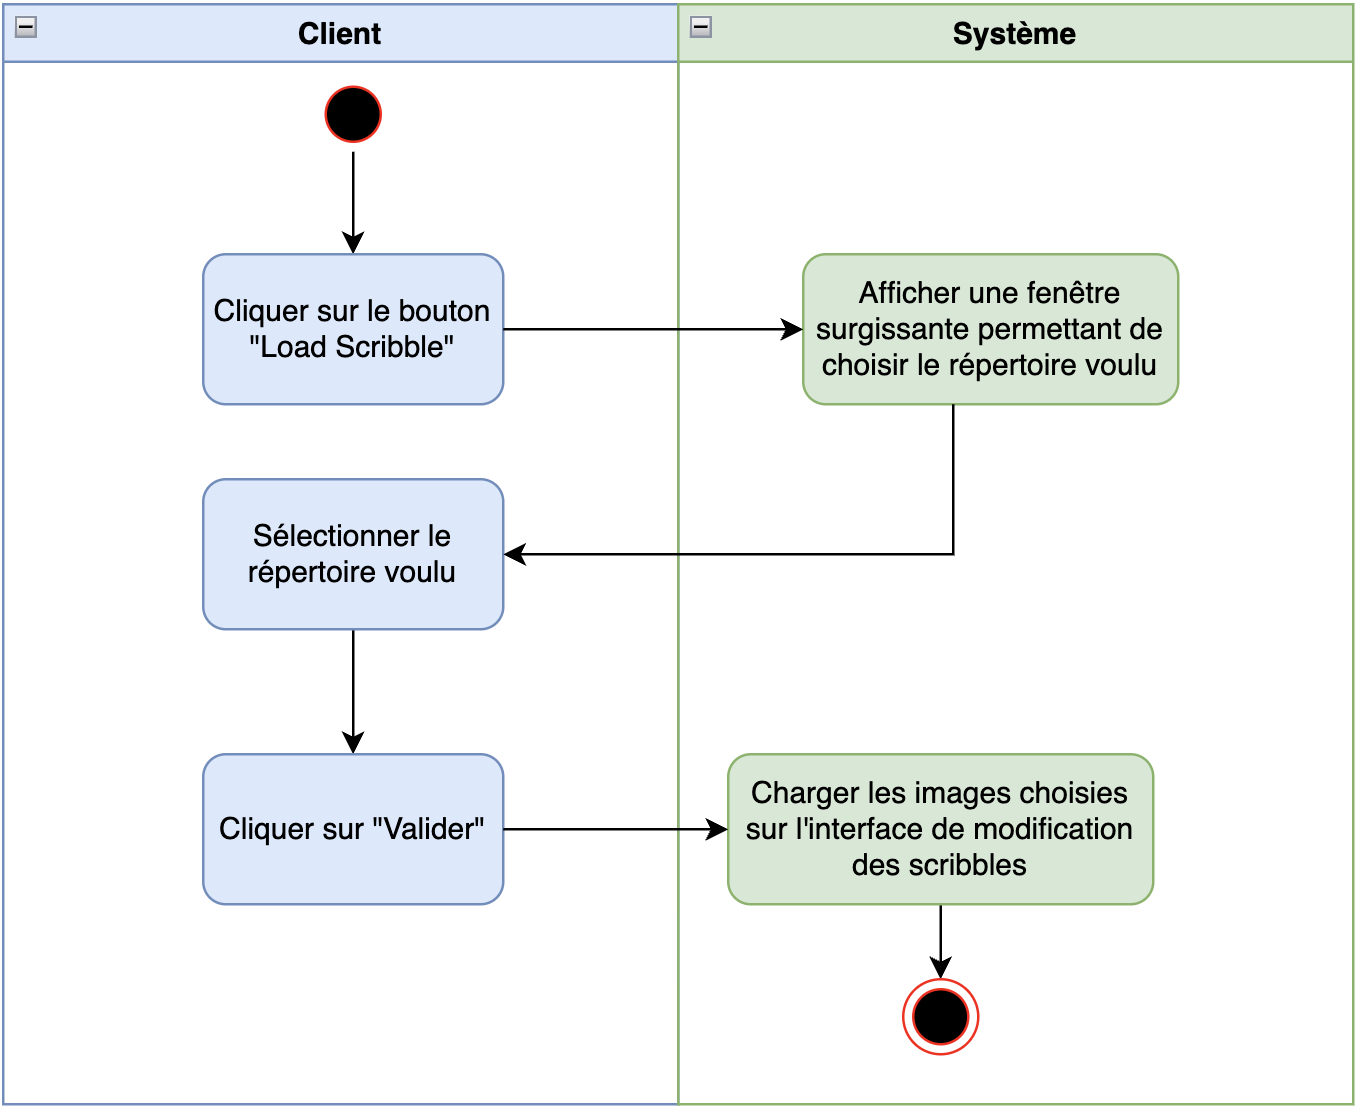
\includegraphics[width=10cm]{scenario-load-scribbles.png}
    \caption{Use case : Diagramme d'activité du scénario de chargement des scribbles}
    \label{fig:scenario-load-scribbbles}
\end{figure}

Une deuxième fonctionnalité que nous pouvons expliciter est \textbf{le choix des dossiers d'images colorisées à visualiser}.
Pour effectuer cette action, l'utilisateur devra se trouver dans la partie "visualiser" de l'interface.
Cette action sera également effectuée par une équipe de chercheurs et n'a aucune dépendance. Elle comporte un seul scénario 
d'utilisation. L'utilisateur doit cliquer sur le champ correspondant au label \textit{directory for original images}. Le système
doit alors afficher une fenêtre qui permet de parcourir les répertoires de l'ordinateur utilisé. Une fois devant cette fenêtre, l'utilisateur
peut alors choisir le répertoire ou l'image voulu et appuyer sur le bouton valider. Le système doit ensuite afficher le nom du répertoire 
sélectionné dans le champ. La condition pour que ce scénario soit valide est que le chemin d'accès existe et corresponde à ce que l'utilisateur a choisi.
La figure \ref{fig:scenario-choix-images-visualiser} illustre le déroulé de cette action.\\

\begin{figure}[htp]
    \centering
    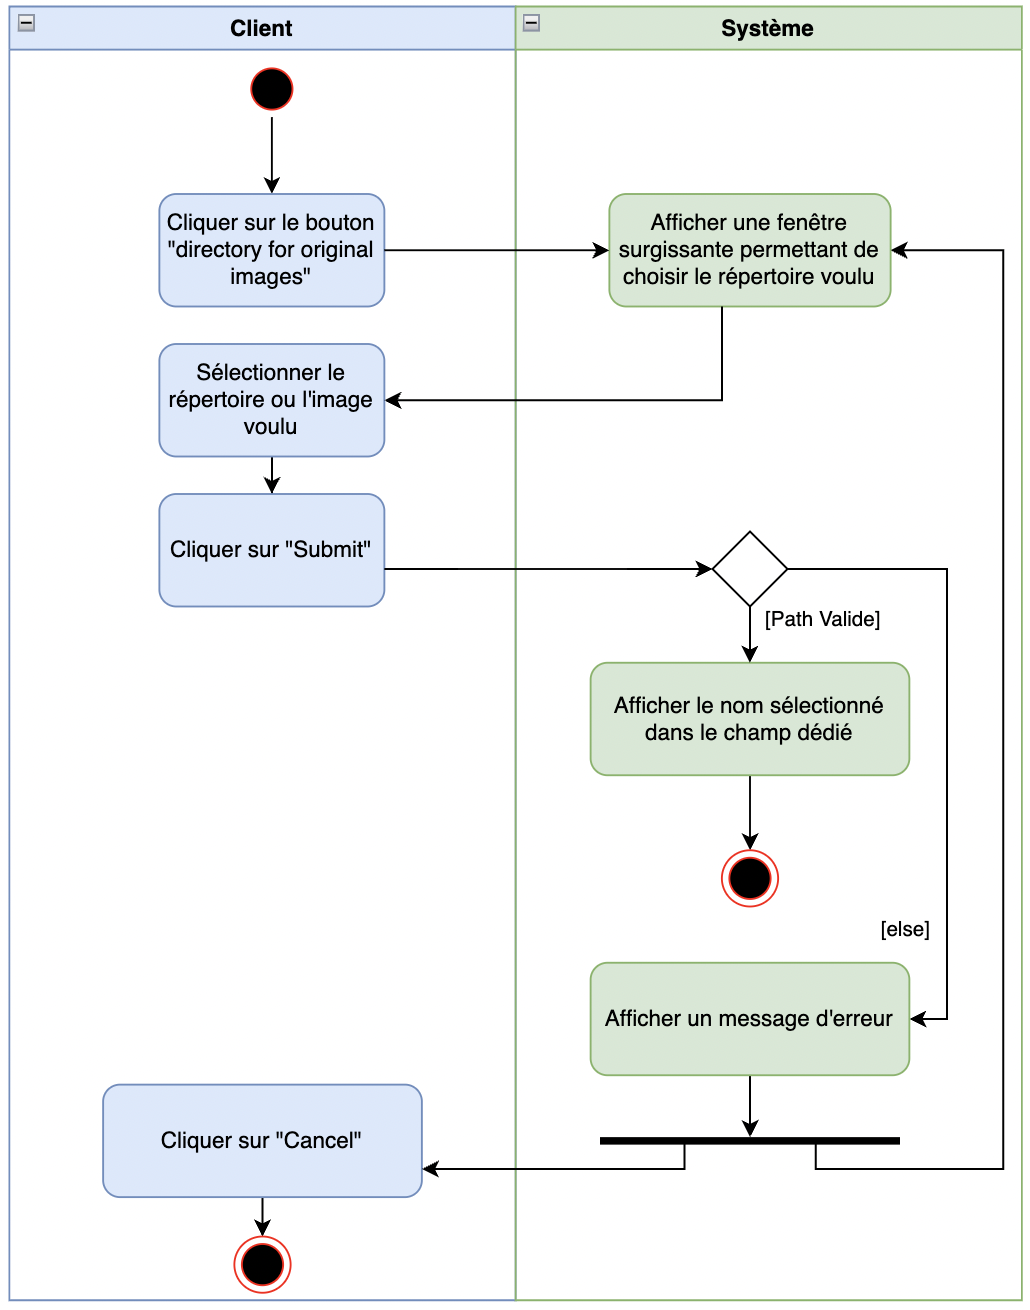
\includegraphics[width=10cm]{scenario-choix-images-visualiser.png}
    \caption{Use case : Diagramme d'activité du scénario de choix des dossiers d'images à visualiser}
    \label{fig:scenario-choix-images-visualiser}
\end{figure}

Le dernier cas que nous détaillons est le cas où l'utilisateur souhaite \textbf{enregistrer une question} lorsqu'il est en train de créer un questionnaire.
Ce cas d'utilisation est dépendant d'autres cas d'utilisation. Il faut en effet que la question ait été créée, que l'on ait spécifié son type et que des champs de réponse aient    
été ajoutés à la question. Ce cas d'utilisation est réalisé par une équipe de chercheurs.
Deux scénarios sont imaginés : un scénario normal et un scénario d'erreur. Lors du scénario normal, l'utilisateur clique sur le bouton 
\textit{save}. Le système doit ensuite vérifier si tous les champs sont correctement remplis, enregistrer la question, actualiser la page avec un formulaire vierge
et afficher un message de confirmation pour l'utilisateur. Le scénario d'erreur est lancé lorsqu'un champ obligatoire n'est pas correctement
rempli. Il faut alors que le système affiche un message d'erreur en indiquant quel champ est mal rempli. Une fois le champ correctement rempli, l'utilisateur
retourne au début du scénario normal.
La figure \ref{fig:scenario-enregistrer-question} décrit ces scénarios.

\begin{figure}[htp]
    \centering
    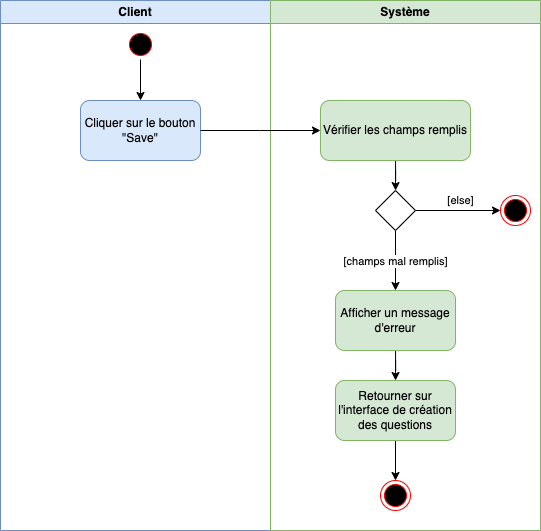
\includegraphics[width=10cm]{scenario-enregistrer-question.drawio.png}
    \caption{Use case : Diagramme d'activité du scénario d'enregistrement d'une question}
    \label{fig:scenario-enregistrer-question}
\end{figure}

Afin d'obtenir des précisions et de faire des estimations sur le temps de chacune des \textit{user stories} et des \textit{use cases},
nous avons établi une liste de tâches qui permet de les décomposer et d'évaluer leur complexité plus facilement.
Ces tâches sont décrites dans la section suivante.


\subsubsection{Précisions des exigences à l'aide de tâches}\label{sec:taches}

Les tâches que nous avons détaillées permettent à l'équipe de développement de comprendre et d'expliciter le travail nécessaire
pour compléter les \textit{user stories}. Elles servent également à estimer plus précisément le temps d'une \textit{user story}.
En effet, l'ensemble de tâches permet de clarifier et de concrétiser ce qu'il y aura à faire.
Seules quelques une de ces tâches seront détaillées dans cette partie afin d'expliquer notre démarche.
L'ensemble des tâches définies se trouve dans la section \ref{sec:annexe-livrable}.\\

Ici, nous allons détailler les tâches que nous avons déterminées pour \textbf{choisir les dossiers d'images colorisées à charger}.
Pour cette fonctionnalité, nous avons défini la liste des éléments suivants à développer :
\begin{itemize}
    \item Un champ pour sélectionner des dossiers avec des images colorisées qui seront à visualiser. (1,5 heure)
    \item Un bouton \texttt{add} qui permettra d'ajouter le dossier sélectionné à la liste des dossiers à visualiser. (1,5 heure)
    \item Un champ qui permet de visualiser la liste des dossiers que l'on va visualiser. (2 heures)
    \item Un bouton à côté de chaque dossier qui a été ajouté qui permet de le supprimer de la liste. (2 heures)
\end{itemize}
Ces différentes tâches très découpées nous ont permis d'estimer le temps total qui sera nécessaire pour compléter la \textit{user story}, soit 7 heures. \\

Nous pouvons faire de même pour la fonctionnalité \textbf{créer une nouvelle configuration de scribbles}.
Les éléments à produire pour la réaliser sont les suivants :
\begin{itemize}
    \item Une interface permettant de créer une nouvelle configuration de \textit{scribbles} en fonction d'un dossier d'image et d'un nom de configuration. (5 heures)
    \item Une interface contenant l'image noir et blanc à coloriser et un bouton de validation des \textit{scribbles}. (3 heures)
    \item Un canvas qui permet de dessiner les \textit{scribbles}. (0,5 heure)
    \item Un \textit{color picker} pour choisir une couleur pour le \textit{scribble}. (0,5 heure)
    \item Une jauge permettant de choisir une taille de traits pour le \textit{scribble}. (0,5 heure)
    \item Un bouton à cocher qui permet d'effacer l'ensemble des scribbles sur une image. (1 heure)
    \item Une gomme qui permet d'effacer les \textit{scribbles}. (2 heures)
    \item Un bouton qui permet de passer de 'faire des traits' à 'faire des points'. (3 heures)
    \item Un bouton qui permet d'enregistrer chacun des \textit{scribbles}. (2 heures)
    \item Un bouton qui permet de sauvegarder et de finaliser la configuration des \textit{scribbles}. (3 heures)
    \item Une arborescence qui permet d'avoir différentes configurations de \textit{scribbles} pour un même dossier d'images. (2 heures)
    \item L'enregistrement des \textit{scribbles} doit se faire avec l'extension demandé par le modèle (par exemple png) et dans le bon dossier de configuration. (4 heures)
\end{itemize}

Ainsi, pour cette fonctionnalité, nous avons estimé un temps total de 34 heures de travail.\\

Ces différentes tâches nous ont permis d'estimer les temps pour les \textit{user stories} mais également pour les différentes parties du projet.
Ainsi, pour la partie d'exécution des méthodes de colorisation depuis l'interface, le temps estimé est de 216,5 heures.
Il est prévu que le temps total passé à développer la partie de visualisation des résultats et des images est de 91 heures.
Enfin les questionnaires devraient prendre environ 86 heures.
Nous remarquons donc que la partie l'aspect de l'exécution des méthodes de \textit{deep learning} depuis l'interface sera la plus importante et 
longue à développer. Cela est dû au fait qu'il faut pouvoir intégrer différents types de méthodes avec leurs fonctionnements particuliers.
Le temps total estimé pour tout le projet est 394 heures. \\

L'analyse fonctionnelle que nous avons réalisée permet de nous donner une vue d'ensemble des fonctionnalités
qui seront à implémenter dans le projet. Elle offre également une vision à différentes échelles : très précises avec 
les tâches, un peu plus générale avec les \textit{use cases} et les \textit{user stories}.
Cette analyse permet également d'avoir différentes perspectives du projet. En effet, les \textit{user stories}
se placent strictement d'un point de vue utilisateur tandis que les \textit{use cases} intègrent également le système.
De plus, la définition des tâches nous a permis en tant que programmeur de concrétiser les exigences et de mieux les évaluer.
Avec cette analyse globale des besoins du client, il est alors possible de commencer à imaginer l'implémentation
et surtout, la structure que prendra cette mise en oeuvre.
L'objectif est alors d'établir un socle architectural qui servira de référence lors du développement et qui
permettra de définir différents modules et leurs interactions. Il s'agit également de définir les outils avec lesquels nous 
allons implémenter la solution. Ce sont ces aspects qui sont expliqués dans les sections suivantes.

\subsection{Modélisation et architecture de la solution}

Dans cette partie, nous allons détailler l'architecture de la solution que nous souhaitons implémenter à différentes échelles.
Premièrement, nous expliquerons la structure que nous avons défini d'un point de vue général, afin d'avoir une vision globale du projet.
Dans une seconde partie, nous exposerons une version plus détaillée de cette structure, afin de comprendre les différents modules et leurs interactions.
Enfin, nous présenterons les outils vers lesquels l'architecture définie nous a conduit.

\subsubsection{Architecture générale de l'application web}

La définition de l'architecture générale est la première étape de l'établissement des spécifications techniques. Elle permet
de définir des fondements techniques qui permettront de répondre aux besoins fonctionnels.
Dans notre cas, nous avons choisi de développer la solution sous la forme d'une application web. Nous avons choisi ce format suite 
à nos discussions avec le client car c'est le format qui permettra de rassembler les questionnaires avec les autres parties de manière simple. En effet les questionnaires devront possiblement être mis en ligne plus tard : une application web est plus pratique pour faire cela.

Comme illustré sur la figure \ref{fig:clientserver}, notre solution est basée sur une architecture client-serveur. 
Cette architecture est un modèle de conception logicielle qui permet de séparer les fonctionnalités de notre application en deux sections distinctes: 
\begin{itemize}
    \item La partie \textbf{client} est responsable de l'affichage des différentes interfaces de notre application, notamment celle permettant la sélection des images à coloriser ou celle responsable de l'affichage des résultats.  Elle prend aussi en charge les interactions des utilisateurs avec ces interfaces.
    \item La partie \textbf{serveur} présente la logique métier de notre application. En effet, cette partie est responsable de gérer les données reçues telles que les images à coloriser puis d'effectuer les traitements nécessaires comme l'exécution des méthodes de colorisation et finalement renvoyer les résultats vers la partie client.
\end{itemize}

L'architecture client-serveur s'est donc avérée être la meilleure solution. En effet, elle nous a permis de séparer les responsabilités de manière efficace et d'assurer la scalabilité de notre application de façon à avoir la possibilité d'ajouter à chaque fois des traitements liés à des autres modèles de colorisation sans modifier la partie qui concerne les utilisateurs. \\

\begin{figure}[htp]
    \centering
    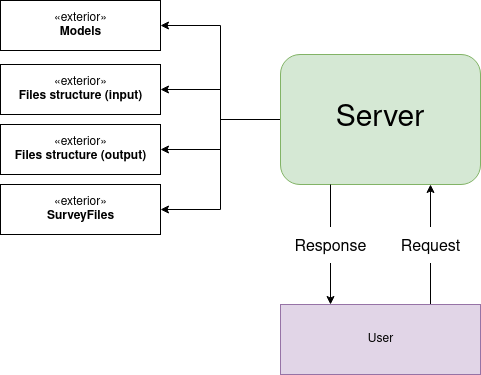
\includegraphics[width=11cm]{code-architecture-client-server.png}
    \caption{Représentation de l'architecture client-serveur}
    \label{fig:clientserver}
\end{figure}

En plus de choisir une architecture pour la conception logicielle de notre application, il est primordial d'opter pour une approche afin de structurer notre code.
Dans ce contexte, nous avons adopté une approche MVC (Modèle-Vue-Contrôleur), visible dans la figure \ref{fig:mvc}, qui sépare notre application en trois composants distincts s'occupant chacun d'une partie spécifique. \\ 

La partie Modèle correspond aux données et à tout traitement logique de ces dernières. Dans notre cas, cette couche est essentielle pour manipuler les images à coloriser. Également, la partie modèle utilisera un module, le plus générique possible, pour accéder aux différents modèles de \emph{deep learning} afin d'orchestrer les colorisations demandées. \\

La couche Vue est responsable de l'affichage des interfaces à l'utilisateur et de la collecte de ses entrées. Ici, il est nécessaire de réaliser des interfaces permettant de paramétrer précisément les colorisations. De plus, il est possible de relever le fait que certains composants de ces interfaces peuvent être utilisés à plusieurs endroits, par exemple le zoom sur des images lors des résultats des colorisations. Aussi, il est important de noter que les colorisations peuvent avoir une durée indéterminée donc il faudrait que la partie Vue soit capable de mettre à jour l'interface dynamiquement en fonction de ces résultats. \\

Enfin, la couche Contrôleur a l'objectif de gérer les interactions entre la vue et le modèle, en prenant en compte les entrées de l'utilisateur et en les transmettant au modèle pour effectuer les traitements nécessaires, puis en transmettant ces données modifiées à la vue pour l'affichage. \\

En fin de compte, cette approche offre une bonne flexibilité et une meilleure gestion de code de façon à pouvoir modifier une partie spécifique sans affecter les données et la logique de notre application, elle est également conçue pour faciliter le développement collaboratif au sein de l'équipe. \\

\begin{figure}[htp]
    \centering
    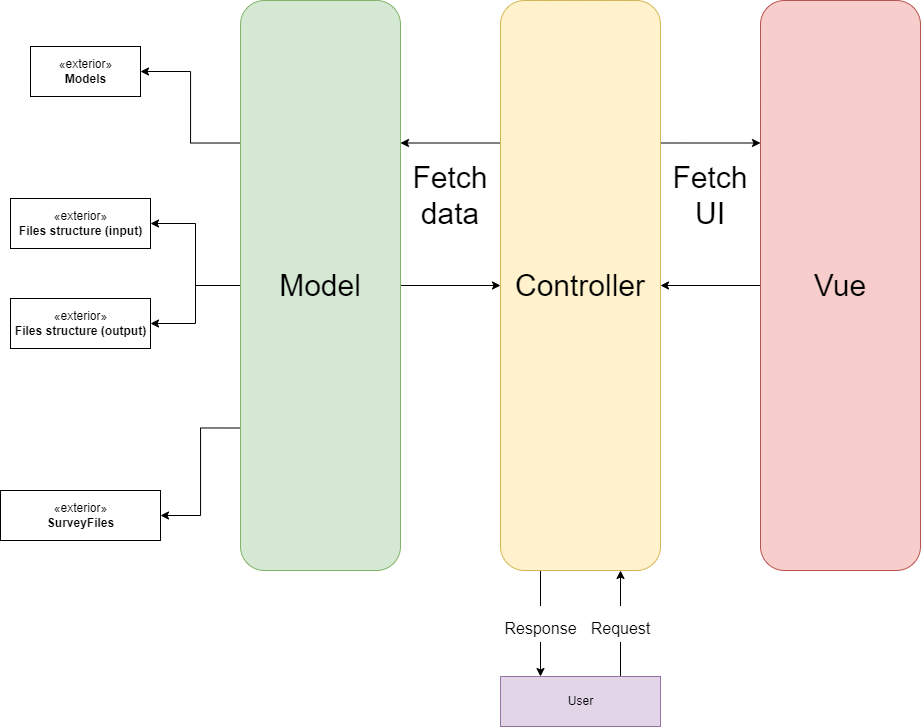
\includegraphics[width=14cm]{code-architecture-mvc.png}
    \caption{Représentation du modèle MVC et des modules interagissant avec dans notre architecture}
    \label{fig:mvc}
\end{figure}

Cette architecture nous donne une vision globale de la solution technique que nous allons adopter.
Nous devons cependant la préciser en définissant différents modules afin que l'ensemble de l'équipe puisse travailler sur des parties différentes tout en ayant une vision globale du projet.

\subsubsection{Définition de modules et de leurs interactions}\label{sec:archi-detaillee}
Dans cette partie, nous allons préciser l'architecture décrite dans la partie précédente en définissant des modules et leurs fonctionnalités principales. 
Nous allons montrer comment ces éléments s'intègrent dans l'architecture MVC et pourquoi ils permettent de répondre aux exigences fonctionnelles du client.

\begin{figure}[!h]
    \centering
    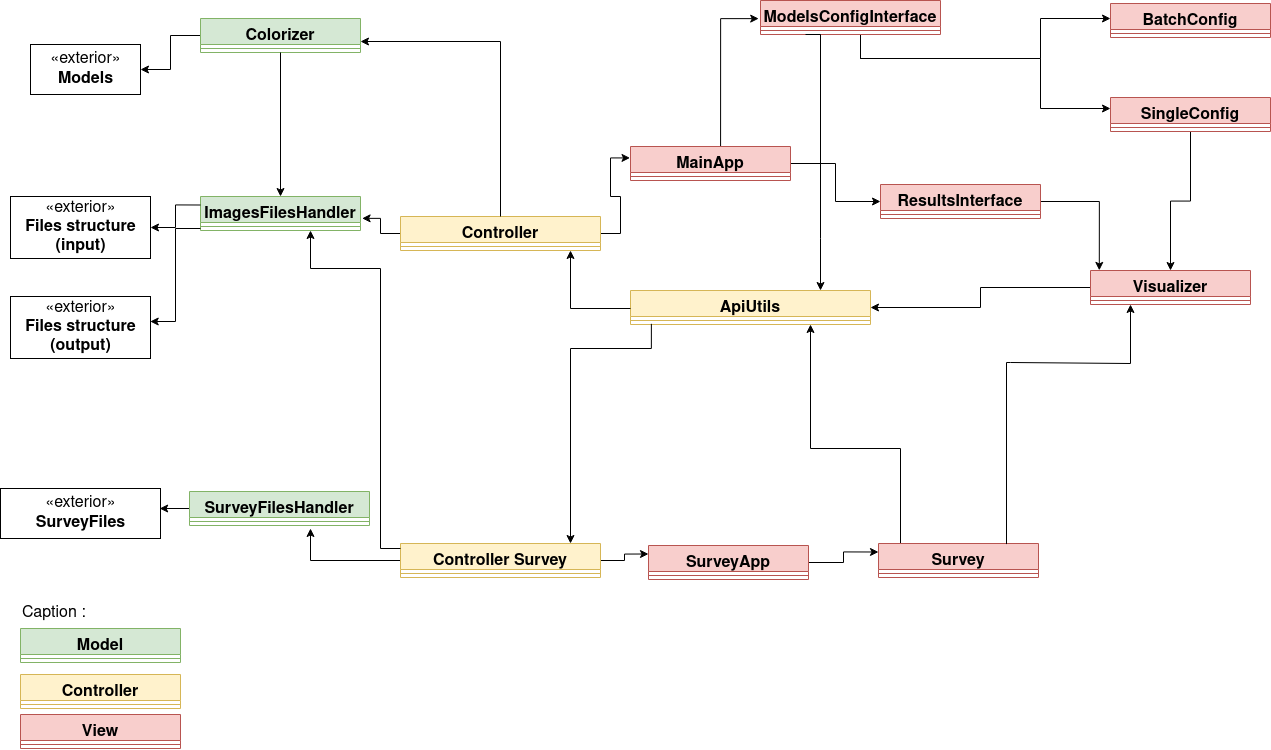
\includegraphics[width=16cm]{code-architecture.png}
    \caption{Architecture du code séparée en trois parties selon le modèle MVC. Chaque partie est découpée en modules.}
    \label{fig:architecture}
\end{figure}

\begin{figure}[!h]
    \centering
    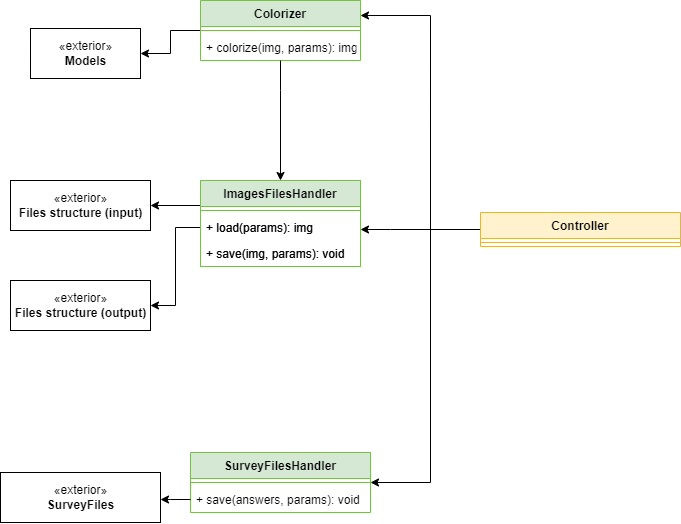
\includegraphics[width=12cm]{code-architecture-model.png}
    \caption{Détails de l'interface de la partie Modèle utilisée par le Contrôleur}
    \label{fig:architecturemodel}
\end{figure}

\begin{figure}[!h]
    \centering
    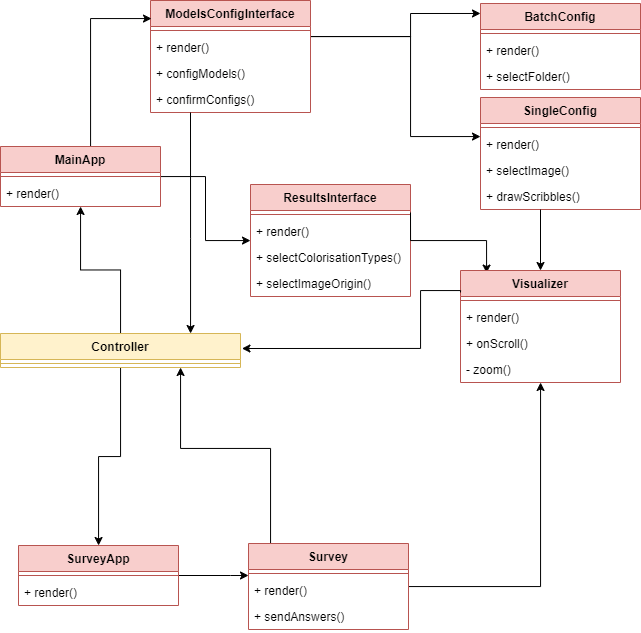
\includegraphics[width=12cm]{code-architecture-view.png}
    \caption{Détails de l'interface entre la Vue et le Contrôleur}
    \label{fig:architectureview}
\end{figure}

\begin{figure}[!h]
    \centering
    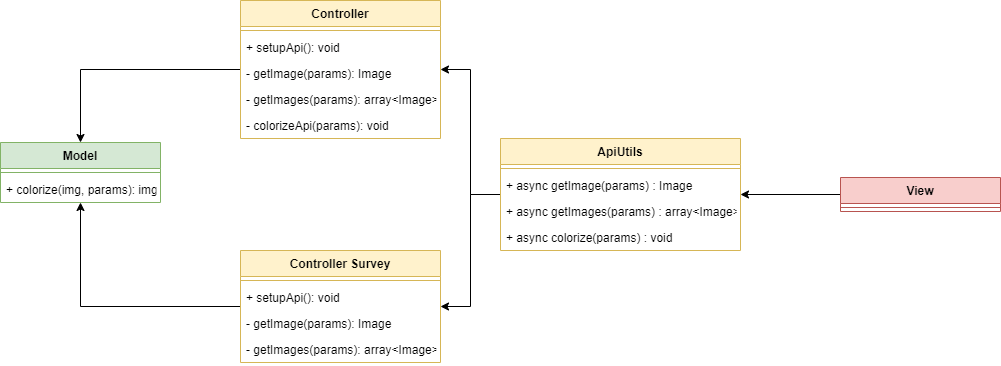
\includegraphics[width=14cm]{code-architecture-controller.png}
    \caption{Détails de l'interface du Contrôleur}
    \label{fig:architecturecontroller}
\end{figure}

Le schéma de l'architecture détaillée est visible sur la figure \ref{fig:architecture}. Nous allons désormais la présenter partie par partie.

Premièrement, pour la partie Modèle (figure \ref{fig:architecturemodel}), on peut différencier 3 modules.
Le premier est \texttt{Colorizer}, représenté en haut à gauche.
Il servira d'interface entre notre code et les intelligences artificielles capables d'effectuer les colorisations. 
Il est important de préciser que chaque intelligence artificielle s'exécute de manière très différente. 
En effet, elles peuvent avoir différents paramètres tels que les scribbles ou la colorisation en fonction d'une image de référence mais également différentes contraintes comme, par exemple, la taille des images. 
Afin de gérer ces spécificités, le module disposera d'une abstraction des modèles d'intelligences artificielles afin de les exécuter de manière uniforme.

Ensuite, les modules \texttt{ImagesFilesHandler} et \texttt{SurveyFilesHandler} permettent d'accéder aux données concernant respectivement les résultats des colorisations et les questions/réponses aux questionnaires.
Ainsi \texttt{ImagesFilesHandler} devra donc charger des images pour les coloriser et enregistrer les resultats de colorisation sur le disque.
Concernant la gestion des images sur le disque, nous avons opté pour une arborescence de fichiers afin de garder une structure simple et de faciliter l'accès aux données.
En effet, une base de données aurait complexifié leurs utilisations en dehors du cadre de ce projet.
Ainsi les informations seront sauvegardées en suivant l'arborescence de fichiers détaillée dans la figure \ref{fig:architecturefiles}.

\begin{figure}[htp]
    \centering
    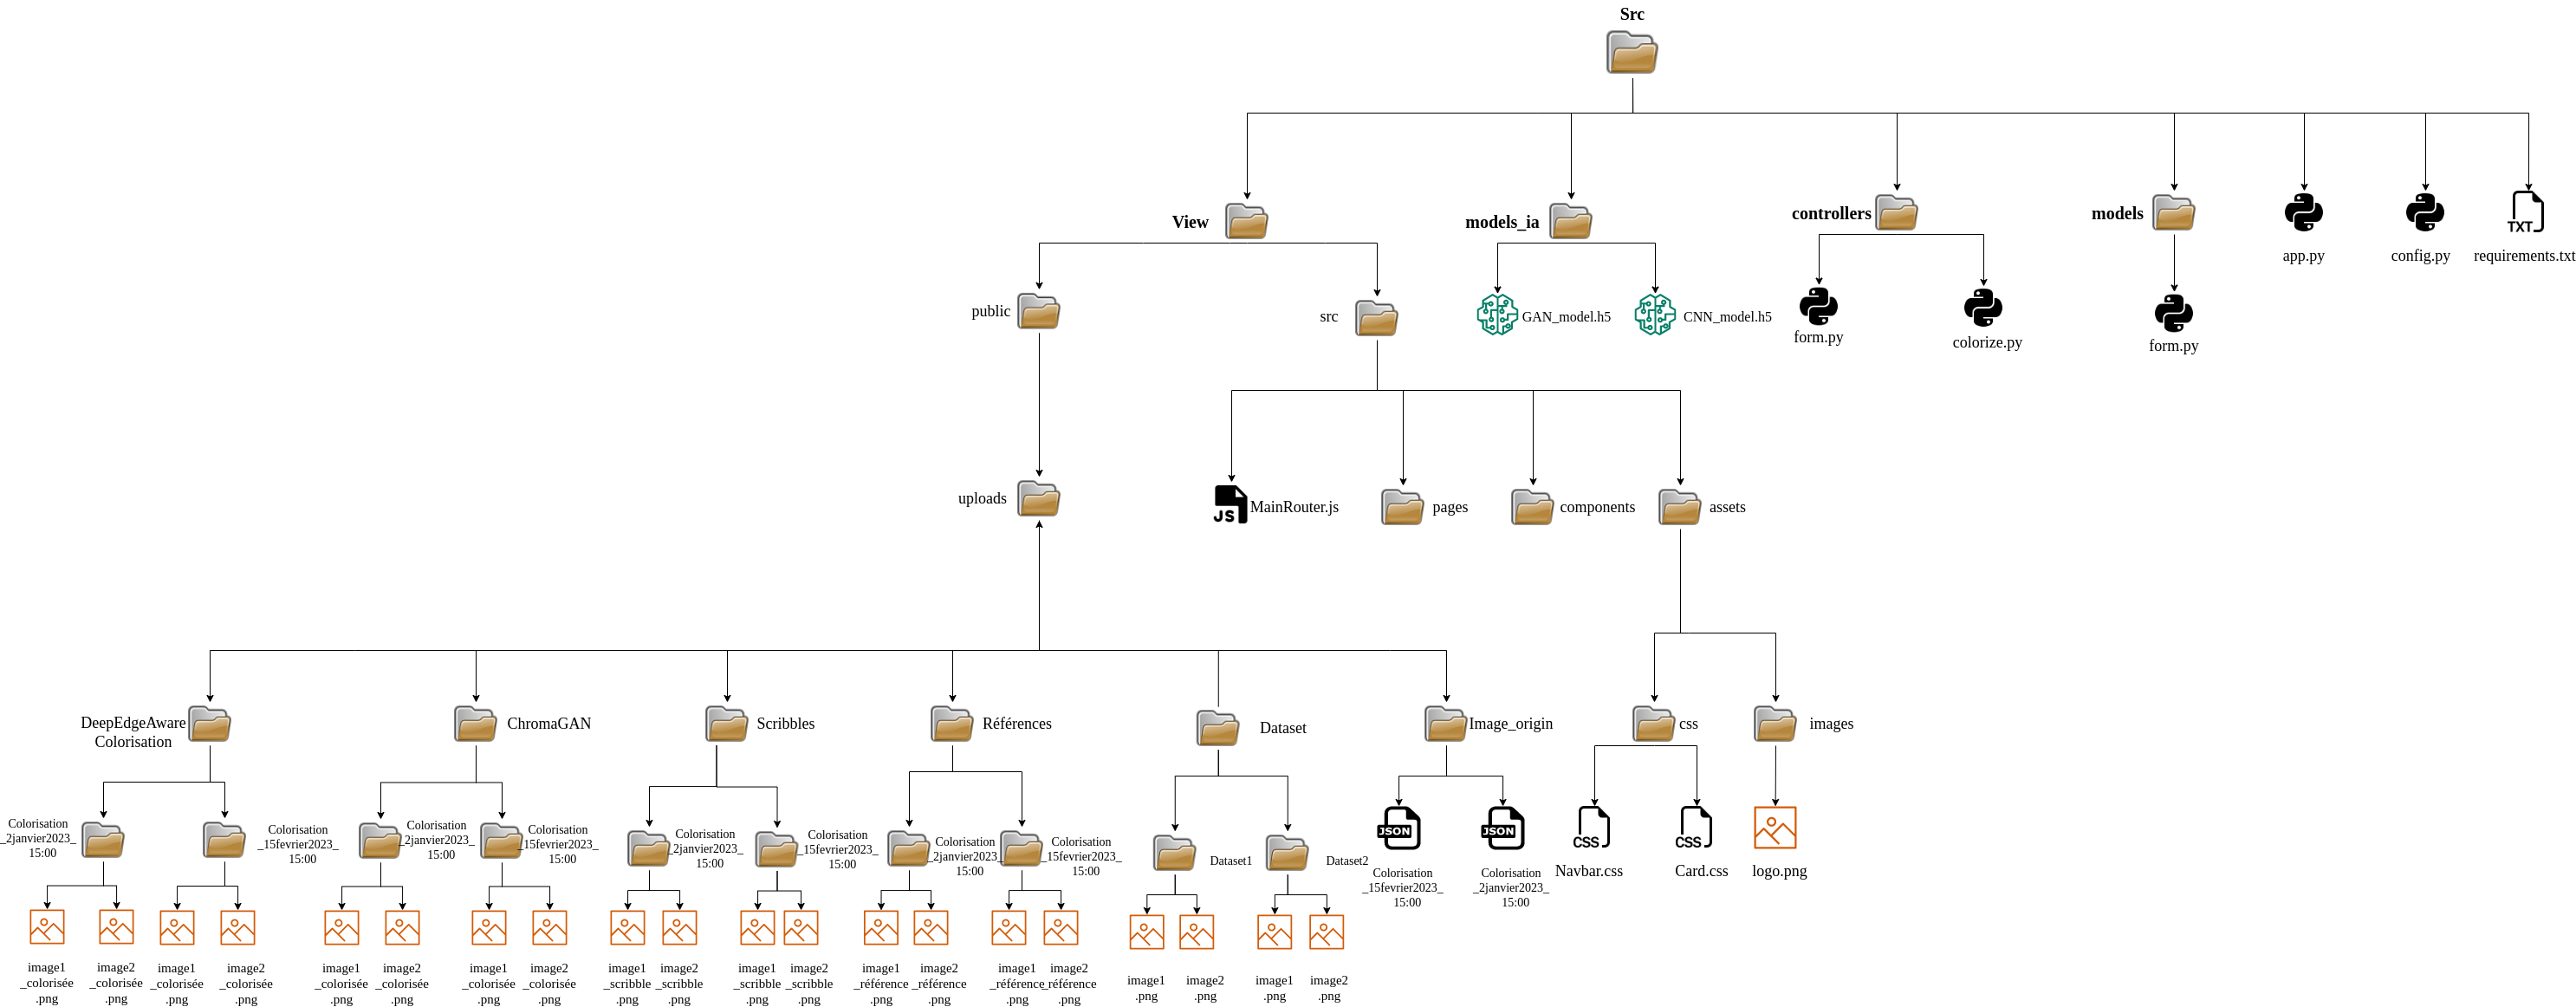
\includegraphics[width=17cm]{code-architecture-files.png}
    \caption{Organisation de l'arborescence des fichiers du logiciel}
    \label{fig:architecturefiles}
\end{figure}

Les données utilisées et générées seront donc stockées dans le répertoire \texttt{src/View/public/uploads}, présent à gauche de la figure \ref{fig:architecturefiles}. 
Ce répertoire est constitué des répertoires \texttt{Dataset}, \texttt{Image\_origin}, \texttt{References}, \texttt{Scribbles} et d'un répertoire par méthode de colorisation. 
Le répertoire \texttt{Dataset} permet de stocker les images d'origine.
Le répertoire \texttt{Image\_origin} est utilisé pour répertorier toutes les colorisations effectuées.
Chaque colorisation génère un fichier json qui renseigne les détails de la colorisation effectuée.
Le répertoire \texttt{References} permet de stocker toutes les images de références pour les méthodes de colorisations qui nécessitent leur utilisation.
Le répertoire \texttt{Scribbles} est présent afin de stocker les scribbles réalisés. 
A noter qu'il sera possible d'avoir plusieurs configurations de scribbles pour un dossier d'images d'origine.
Les répertoires présents pour chaque méthode de colorisation sont utilisés pour stocker les images générées grâce aux méthodes de colorisation.
Les données des questionnaires seront également stockées sur le disque à l'aide de fichiers \texttt{json}.

Dans chacun de ces répertoires, lorsque des données sont générées, elles sont nommées avec leur date de génération afin de ne pas écraser des données déjà présentes. 
Par exemple, si l'on effectue une colorisation de plusieurs images avec le modèle ChromaGAN le 15 janvier 2024 à 16h00 alors les résultats se trouveront dans le répertoire suivant : \texttt{/public/uploads/ChromaGAN/Colorisation\_20240115\_16-00}.

Cette gestion des données nécessite la présence des modules \texttt{ImagesFilesHandler} et \texttt{SurveyFilesHandler} afin de faciliter leur accès dans le code de la partie Modèle. \\

Deuxièmement, la partie Vue, illustrée par la figure \ref{fig:architectureview} concerne la production des interfaces utilisateurs (frontend).
Elle comporte deux composants principaux, un pour chaque application : \texttt{MainApp} pour la colorisation et l'affichage des résultats de celles-ci et \texttt{SurveyApp} afin de créer, répondre et afficher les résultats des questionnaires.

On peut voir sur la figure \ref{fig:architecture} que ces deux composants sont directement liés à leur contrôleur respectif, mais aussi aux autres composants de la partie Vue (par exemple, \texttt{ModelsConfigInterface} ou \texttt{Survey}). 
En effet, ces deux composants ré-utilisent d'autres composants qui correspondent à des morceaux de l'interface.
On note que le composant \texttt{Visualizer} sera utilisé dans les deux applications et qu'il faudra donc permettre de le paramétrer en fonction du contexte. \\

Troisièmement, la partie Contrôleur est divisée en deux sous-parties visibles sur la figure \ref{fig:architecturecontroller}. 
Elle doit orchestrer les parties Modèle et Vue, c'est à dire par exemple envoyer les données à afficher dans les différentes interfaces ou effectuer du côté du serveur les actions liées aux boutons.
La première sous-partie est constituée de deux contrôleurs. \texttt{Controller} pour l'application de colorisation et \texttt{ControllerSurvey} pour celle des questionnaires. 
Ils auront la charge d'exécuter les méthodes présentes dans la partie modèle.
Pour cela, ils permettront de faire des requêtes HTTP à certaines URL données, appelées \emph{endpoints}, qui correspondront chacune à une action à effectuer. 
Ce principe s'appelle une \emph{API} et permet d'avoir une interface entre les Vues et les Modèles.
La deuxième sous-partie, correspondant à \texttt{ApiUtils}, contiendra des méthodes facilitant l'accès à l'ensemble de méthodes présentes dans \texttt{Controller} et \texttt{ControllerSurvey} afin de limiter la complexité du code dans la partie Vue.

\subsubsection{Technologies permettant de répondre aux exigences}

Le choix des technologies qui seront utilisées pour développer la solution est complexe. En effet, il faut s'assurer que les
technologies choisies correspondront à l'architecture conceptuelle de la solution mais aussi, permettront de répondre aux exigences du client
(aussi bien fonctionnnelles que non fonctionnelles). Il faut également choisir des technologies qui sont comprises et assez maitrisées par l'équipe
de développement. Ce dernier point est également très important car il diminue le temps passé à se familiariser avec les technologies et facilite le développement. 
Dans le développement de la solution web imaginée, nous avons choisi d'utiliser les technologies \texttt{ReactJS} pour le \textit{front-end} et  \texttt{Flask} pour le \textit{back-end}.\\

Pour le \textit{back-end}, nous voulions une technologie qui soit en \texttt{Python} pour plusieurs raisons. Tout d'abord \texttt{Python} est un langage de programmation qui
est très bien maitrisé par tous les membres de l'équipe. De plus, la plupart des modèles de colorisation d'images sont implémentés en \texttt{Python}. Pour simplifier leur intégration
dans notre application, nous souhaitions donc que la solution soit réalisée dans le même langage.
\texttt{Flask} est donc un framework \texttt{Python} léger et flexible pour le développement d'applications web. Dans notre cas, \texttt{Flask} est utilisé  pour la gestion des données et la logique de l'application. 
Nous avons choisi d'utiliser \texttt{Flask} par rapport à d'autres technologies \texttt{Python} car il est minimaliste et rapide. En effet, d'autres technologies plus complexes auraient pu être choisies pour 
cette partie, comme par exemple \texttt{Django}. Cependant, \texttt{Django} est un framework très complet, qui contient par exemple des ORM permettant de faire un lien direct avec une base de données.
\texttt{Django} est moins rapide et moins flexible. Notre projet n'intégrant pas de bases de données, nous avons fait le choix de \texttt{Flask} et de sa flexibilité.\\

De son côté, \texttt{ReactJS} est une bibliothèque \texttt{JavaScript} pour la création d'interfaces utilisateur interactives et modernes ce qui va nous permettre d’implémenter la partie client.
Ce choix est dû à sa performance élevée qui permet de mettre à jour efficacement les composants de l’interface en se basant sur le concept du DOM virtuel.
Ce choix est également dû au fait que c'est une technologie qui est bien maitrisée par une partie de l'équipe et qui sera donc facilement intégrée au projet. \\

Cette combinaison de technologies nous donne donc la possibilité de tirer parti de la puissance de \texttt{ReactJS}  pour la partie client tout en utilisant \texttt{Flask} pour la partie serveur de manière efficace.
La figure \ref{fig:outils} illustre l'intégration de ces technologies dans l'architecture client-serveur du projet.

\begin{figure}[htp]
  \centering
  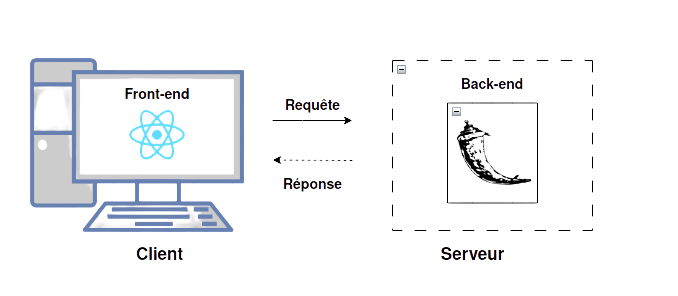
\includegraphics[width=11cm]{outils.png}
  \caption{Intégration des technologies dans l'architecture du projet}
  \label{fig:outils}
\end{figure}


\section{Gestion de projet}

Dans cette partie, nous nous intéressons à la manière dont le projet sera conduit. Définir une organisation
et une approche claires sont des aspects aussi importants que la spécification des besoins ou de l'architecture.
En effet, c'est en s'appuyant sur des méthodes et des règles définies et partagées par tous, aussi bien par le client que par l'équipe,
que le projet pourra se dérouler avec le moins d'ambiguïtés possible. Elles permettent à toute l'équipe 
de se synchroniser et de gagner en temps et en efficacité.
Le projet sera conduit selon des méthodes agiles, qui préconisent de courtes itérations (également appelées \textit{sprints})
pour réaliser une partie des objectifs et faire le point avec le client en suivant.
Nous allons donc tout d'abord détailler le déroulement de ces \textit{sprints} en section \ref{sec:sprints}.
Ensuite, en section \ref{sec:validation}, nous expliquerons la manière dont le produit et les fonctionnalités seront validés.
De plus, nous expliciterons les rôles des membres de l'équipe, nos moyens de communication ainsi que notre capacité de travail sur tout le projet
en section \ref{sec:description-equipe}. Afin d'avoir une vision globale du déroulement du projet, nous avons également réparti les tâches
sur la durée du projet en section \ref{sec:gantt}.
Enfin, il est également essentiel d'estimer les risques qui peuvent survenir lors du déroulement du projet,
pour tenter de prévoir des actions pour y remédier. C'est ce qui est réalisé en section \ref{sec:risques}.

\subsection{Déroulement des sprints}\label{sec:sprints}

Comme mentionné, le développement du projet sera réalisé par itérations. 
Une itération, ou \emph{sprint}, est une période de temps fixe durant laquelle l'équipe de développeurs réalise un certain nombre de tâches. À la fin de cette période, une réunion est organisée avec le client pour lui présenter l'avancement et lui donner un nouveau livrable fonctionnel.
Comme illustré dans la figure \ref{fig:sprint-workflow}, il y a 3 étapes importantes dans l'organisation d'un \textit{sprint}.

En premier lieu, l'équipe de développement se réunira pour décider ce qui sera fait durant l'itération : pour cela les tâches dont la priorité sont la plus haute seront extraites du \emph{product backlog}, le document répertoriant les tâches à réaliser, et seront ajoutées au \emph{sprint backlog}. Celui-ci définira ce qui sera développé durant l'itération. En fonction de la durée estimée de ces tâches, une date de fin de sprint sera fixée, en accord avec le client. Une itération classique devrait durer 2 semaines ; cependant, selon l'ampleur du travail à accomplir et les disponibilités de chacun, cela pourra être adapté au moment du début du sprint.
L'équipe projet va ensuite se répartir le travail. Il est important de noter que cette répartition ne sera pas fixe : chaque développeur pourra changer de tâche(s) au cours du \emph{sprint} si cela permet de faciliter le développement.

La mise en oeuvre pourra ensuite commencer, et durer jusqu'à la date de fin de \emph{sprint} décidée à l'avance. Durant cette phase, des réunions régulières (tous les 3 à 4 jours) appelées \emph{daily scrums} seront organisées dans l'équipe de développement pour rester informé de l'avancement de chacun et déceler les éventuelles difficultés et retards pour y remédier au plus vite. Une réunion avec l'encadrant du projet sera aussi prévue au cours de chaque \emph{sprint} afin de s'assurer que le projet se déroule correctement.

Enfin, lors de la réunion avec le client à la fin du \emph{sprint}, l'équipe présentera ce qu'elle a pu réaliser, ce qu'il manque ou ce qui a été ajouté. Un livrable fonctionnel, contenant toutes les nouvelles fonctionnalités développées, sera donné au client. Celui-ci va alors évaluer le résultat en fonction de ses attentes. Si ce qui a été réalisé ne lui convient pas ou que ses besoins ont évolué, le \emph{product backlog} sera mis à jour selon ses remarques. Sinon, les tâches réalisées en seront enlevées.
L'équipe de développement fera aussi une réunion en interne, appelée \emph{sprint retrospective}, pour discuter du déroulement du \emph{sprint} passé. Cela servira à identifier les problèmes rencontrés et mettre en place des solutions pour ne plus les rencontrer par la suite. Une fois cette réunion terminée, l'organisation du prochain \emph{sprint} pourra commencer.


\begin{figure}[!h]
    \centering
    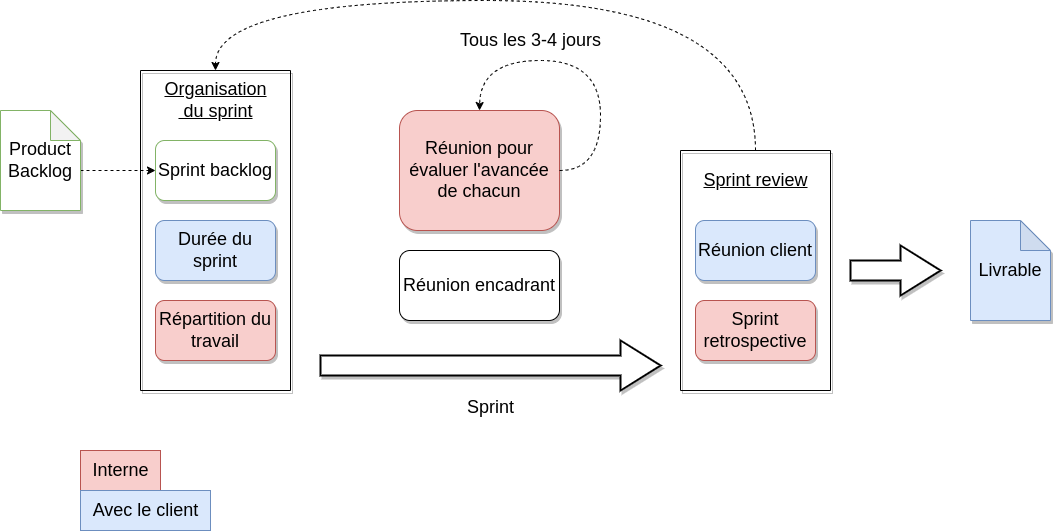
\includegraphics[width=11cm]{sprint-workflow.png}
    \caption{Déroulement du développement par itérations (\emph{sprints})}
    \label{fig:sprint-workflow}
\end{figure}

\subsection{Validation du produit} \label{sec:validation}
La validation du livrable sera effectuée en utilisant plusieurs approches.
\subsubsection{Vérification du fonctionnement par les tests}
La validation du projet se fera notamment par des tests. Les tests prévus se situent à différents niveaux et permettent de vérifier différents
aspects du projet.

Tout d'abord, les tests les plus basiques que nous allons réaliser seront les tests unitaires qui vont servir à tester chaque fonction individuellement et à vérifier qu'elles produisent les résultats attendus.
Les tests unitaires sont très importants car ils permettent de tester toutes les fonctions très précisément.
Lors des tests unitaires, nous allons donc vérifier que les fonctions renvoient bien le résultat attendu dans des cas usuels d'utilisation, mais
également dans des cas d'erreurs. Ces tests sont réalisés par les développeurs, souvent par ceux qui auront codé la fonction qu'ils souhaitent tester et sont donc réalisés pendant les sprints. Si du \textit{Test driven development} est mis en place, ils seront codés avant même que la fonction soit écrite, sinon 
ils sont réalisés une fois la fonction implémentée. Ces tests permettront de montrer au reste de l'équipe que le code écrit est fonctionnel et pourront même servir de documentation
car ils peuvent indiquer à l'équipe le comportement attendu des fonctions. 
Dans notre projet, nous devons réaliser deux types de tests unitaires : ceux pour les fonction écrites pour le backend en \texttt{Python} et ceux pour celles du frontend en \texttt{Javascript}. Nous allons donc utiliser deux outils différents.
Pour réaliser les tests unitaires du backend avec \texttt{Flask}, nous choisissons d'utiliser \texttt{Pytest} qui offre plusieurs fonctionnalités qui facilitent ces vérifications telles que la détection automatique des tests, les assertions personnalisées et la paramétrisation des tests. 
%Avec Pytest nous pouvons tester si le chargement de l'image se fait correctement dans le dossier dédié et vérifier que la colorisation est faite avec le modèle choisi par l'utilisateur. 
%Aussi nous avons choisi Pytest car il supporte les tests asynchrones qui vont nous servir à utiliser des bibliothèques asynchrones pour que nous puissions par exemple de tester si la colorisation de plusieurs images est faites de manière paralelle en lancant la colorisation de chaque image sur un thread où il s'exécute indépendamment du programme principal et du coup l'utilisateur ne sera pas obligé d'attendre la terminaison de la colorisation pour utiliser les autres fonctionnalités de l'application.
Pour la partie frontend avec \texttt{React}, nous avons choisi \texttt{Jest} qui est un outil fourni avec \texttt{React} %et conçu pour être utilisé avec React et 
et il permet de prendre en charge les fonctionnalités de test de ses composants. %\texttt{Jest} se distingue qu'il exécute les tests rapidement en utilisant un mécanisme de mémoire cache. Cet outil permet aussi de réaliser des tests asynchrones ce qui va nous aider à tester le blocage de l'interface utilisateur lorsque l'utilisateur essaye de télécharger des images volumineuses sur l'application. 
%Également nous pouvons vérifier si les traitements sur les images téléchargées peuvent être appliqués en parallèle  sans bloquer l'interface utilisateur et dans un temps rapide à cause du mécanisme de mémoire cache. \\
Ces tests seront réalisés en grand nombre et doivent être impérativement écrits peu de temps après avoir développé la fonction, afin de pouvoir la considérer comme correcte et de l'intégrer au projet. \\

De plus, pour la validation du livrable, nous allons implémenter des tests d'intégration qui servent à vérifier la bonne coordination et la compatibilité entre les fonctionnalités et les modules développés. 
Ces tests sont réalisés par l'équipe et sont des tests qui, comme les tests unitaires, sont codés dans un langage de programmation.
Ils sont implémentés à chaque fois que plusieurs modules ont été finalisés et peuvent donc potentiellement être réalisés à la fin d'un sprint.
Lors de ce type de test, il est possible d'utiliser des \textit{mock} qui permettent de simuler le fonctionnement d'un module ou d'un objet. Ils servent donc à tester un module qui dépend d'un autre, même si ce 
dernier n'a pas encore été implémenté.\\


Des tests fonctionnels aussi vont être créés pour vérifier si l'application répond aux exigences fonctionnelles spécifiées par le client. Ce sont des tests qui permettent de vérifier des besoins directement depuis l'interface de 
l'application. Ces tests peuvent par exemple servir à vérifier l'insertion d'une image, la colorisation d'un dossier d'image ou encore faire un zoom sur une image. Ces tests seront réalisés par l'équipe de développement, une fois qu'une fonctionnalité aura été développée.
Ils peuvent donc être réalisés à la fin d'un sprint et constituent une partie essentielle du projet. En effet, ils permettent de se placer du point de vue d'un utilisateur de l'application et donc de confirmer qu'une fonctionnalité est correcte et répond bien aux \textit{user stories}.
Ce sont des tests essentiels et ils participent à déterminer que l'implémentation d'une \textit{user story} est terminée. Ils permettent de vérifier les critères définis dans la définition du \textit{done}.
Ces tests seront faits manuellement. Cependant effectuer ce type de tests est très chronophage, il est donc possible de penser à les automatiser en utilisant des outils comme \texttt{Selenium}. 
%Nous avons choisi \texttt{Selenium} pour ce genre de test car il nous offre plusieurs fonctionnalités avancées qui facilitent l'écriture du code des tests. 
Cet outil prend en charge de nombreux navigateurs ce qui peut nous aider à tester l'application sur différents environnements et détecter s'il y a une erreur de fonctionnement. 
\texttt{Selenium} supporte aussi les deux languages que nous avons choisi ce qui peut nous permettre soit d'écrire le code manuellement en utilisant le language que nous voulons, soit de faire ces tests d'une manière automatisée en utilisant l'interface utilisateur qui permet de simuler des actions comme par exemple le clic sur le bouton de colorisation d'une image.\\ % traçage des scribbles et la saisie des données dans les champs de textes du questionnaire d'évaluation. 
%Nous avons choisi \texttt{Selenium} aussi car il peut être intégré avec les outils Jest et JUnit pour effectuer des tests d'intégration automatisés.

Enfin d'autres types de tests peuvent être imaginés. Par exemple, des tests de performance peuvent être mis en place pour mesurer les temps de réponse de chaque fonctionnalité et ainsi vérifier si elle répond bien à certaines
exigences non fonctionnelles. Par exemple, ces tests permettent de vérifier le temps de chargement d'un dossier d'image ou encore le temps de colorisation. 
Nous voulons également pouvoir tester la qualité du code. Ainsi, pour détecter les \textit{codes smells} (code mort, dupliqué ou trop long par exemple) et améliorer la qualité de code, nous pouvons utiliser \texttt{SonarQube} qui utilise des règles de qualité de code prédéfinies. Cet outil détecte par exemple les méthodes qui ont un nombre élevé de lignes de code.
%Pour réaliser un code propre et avec une bonne qualité, nous allons fixer avec le client un seuil de code smells à ne pas dépasser.
%Donc nous essaierons de lancer le site depuis plusieurs machines et d'essayer à simuler des charges élevées sur l'application. 
%En cas de besoin, nous pouvons réaliser ces tests en utilisant l'outil \texttt{Apache JMeter} qui est conçu pour générer des charges élevées sur l'application et permet de simuler plusieurs utilisateurs pour le but de tester la scalabilité de l'application et de mesurer les performances sous charge élevée. 


% La validation de livrable sera effectué aussi en utilisant des tests de sécurité qui servent à détecter les failles de sécurité dans l'application. 
% Nous allons utiliser SonarQube qui nous permet d'identifier l'existence des faiblesses de sécurité en utilisant les règles de sécurité prédéfinies. 
% Ces règles sont basées sur des normes de sécurité connues citons par exemple SANS Top 25 et OWASP. 
% Ces genres de tests peuvent vérifier par exemple si l'application protège correctement les images téléchargées par les utilisateurs et s'ils sont stockées et cryptées d'une manière sécurisée pour éviter les fuites de données.

\subsubsection{Le rôle du client dans la validation}

Dans la partie précédente, nous avons vu que de nombreux tests seront réalisés par l'équipe de développement afin de s'assurer du bon fonctionnement de l'application.
Cependant, le client a également un rôle essentiel dans les tests et réalise des tests de recette. Ces tests de recette sont des tests globaux lors desquels le client
simule le comportement d'un utilisateur.
Le rôle du client est donc essentiel pour vérifier que ce qui a été développé correspond bien à ses attentes.
Ainsi, à la fin de chaque sprint, une réunion et une démonstration seront planifiées pour que le client valide ou non le produit selon ses exigences.
Ces tests peuvent aboutir à des demandes d'évolution de l'application et de certaines de ses fonctionnalités si le client réalise 
que ce qui a été développé ne correspond finalement pas à ce qu'il souhaitait.
Ils sont essentiels car ce sont eux qui permettent de confirmer les fonctionnalités développées.\\

La figure \ref{fig:workflow-tests} résume la manière dont les tests seront effectués et la personne qui les réalisera.

\begin{figure}[!ht]
    \centering
    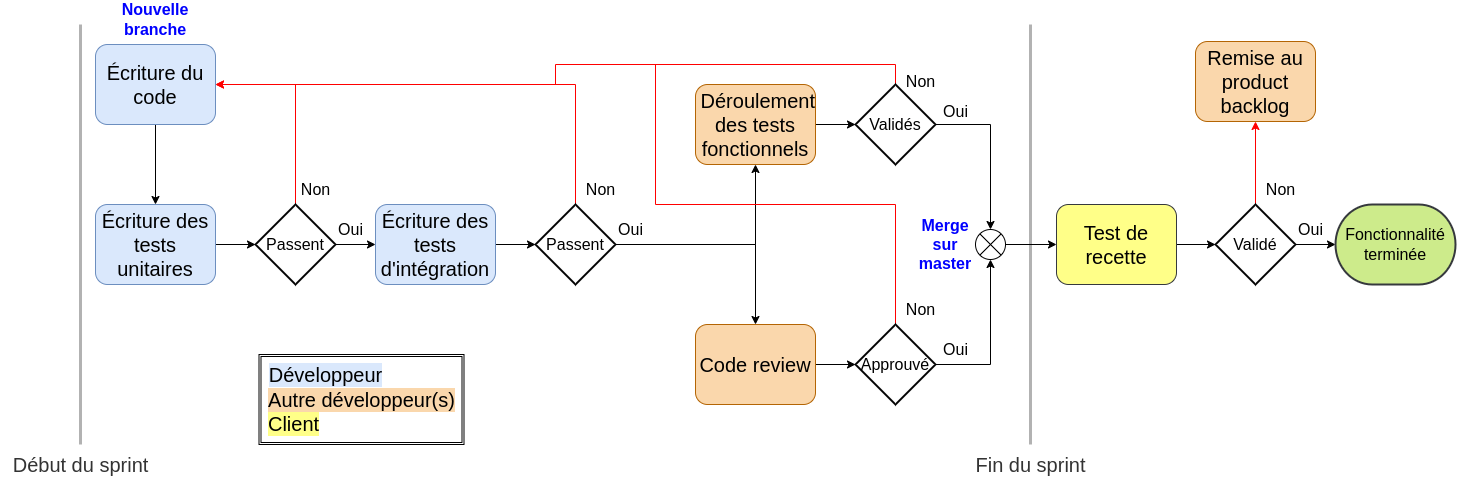
\includegraphics[width=15cm]{Dev-Workflow-PFA.drawio.png}
    \caption{Intégration des tests dans le \textit{workflow}}
    \label{fig:workflow-tests}
\end{figure}

Comme nous pouvons le voir, ce sont d'abord les tests unitaires puis les tests d'intégration qui sont codés
et exécutés par le développeur qui a écrit le code qu'on souhaite évaluer. Ces tests sont écrit dans un langage de programmation.
Si ces deux types de tests passent, alors le code est relu par un autre développeur qui lui exécute des tests fonctionnels sur ce qui a été développé.
Ces tests ne sont pas codés dans un langage de programmation. Une fois que la fonctionnalité a été validé par un autre membre de l'équipe,
le code est ramené sur la branche principale du dépôt (\textit{master}). À la fin du sprint, c'est le client qui teste la fonctionnalité développée. Si elle n'est pas 
validée, elle devra être retravaillée et n'est donc pas enlevée du \textit{Product Backlog}.

\subsection{Description de l'équipe} \label{sec:description-equipe}
Dans un projet informatique utilisant une méthodologie agile, 
l'équipe est généralement composée d'un petit groupe de personnes ayant des compétences multiples et des rôles polyvalents. Les rôles sont souvent plus flexibles et moins hiérarchiques que dans d'autres méthodologies de gestion de projet. Dans notre projet, 
les principaux rôles incluent :
\begin{itemize}

    \item \textbf{Scrum Master :} Ce rôle est similaire à celui de chef de projet, mais il est responsable de faciliter les réunions, de s'assurer que l'équipe respecte les rituels et les principes de \textit{Scrum}, et de résoudre les problèmes qui peuvent survenir.
    \item \textbf{Product Owner :} Ce rôle est responsable de définir les besoins du client et de prioriser les éléments du produit. Il est le représentant du client au sein de l'équipe et s'assure que le produit final répond aux besoins. Pour notre cas, tous les membres de l’équipe sont responsables des besoins du client.
    \item \textbf{Équipe de développement :} Ils sont responsables de la conception, de la construction et de la livraison des fonctionnalités
    \item \textbf{Stakeholder :} Ce sont les personnes qui ont un intérêt dans le projet, dans notre cas il s’agit du client.

\end{itemize}
Chacun de ces rôles peut être occupé par une ou plusieurs personnes à la fois, et ils peuvent être partagés ou combinés selon les besoins du projet.


L'estimation du nombre de jours/hommes pour un projet est importante car elle permet de définir les délais et les coûts pour la réalisation du projet. Cela permet au \textit{Scrum Master} de planifier efficacement le projet. Elle permet également de fixer des objectifs réalisables et de définir des jalons importants pour l'avancement du projet. 
Cette estimation dépend de plusieurs facteurs, notamment la complexité du projet, les compétences et l'expérience des membres de l'équipe, ainsi que les incertitudes et les risques liés au projet. Pour cela on a eu recours à utiliser une méthode qui consiste à décomposer le projet en tâches plus petites puis à estimer la durée de chaque tâche en utilisant les connaissances et l'expérience des membres de l'équipe pour réaliser cette tâche.

Pour ce faire, l'équipe de développement, y compris le \textit{Scrum Master}, sont divisées en trois sous-équipes, chaque équipe est responsable de l'exécution d'une tâche spécifique, et chaque membre de la sous-équipe effectue une sous-tâche de la tâche principale assignée.
Nous prévoyons 3 à 5 heures de travail pour chaque membre de l'équipe par semaine, pour un total de 14 semaines de projet, ce qui donne 42 à 70 heures de travail par membre pour le projet entier. Sur la phase de réalisation,
7 membres de l'équipe travailleront sur le projet. Nous pouvons donc estimer la capacité de travail totale entre 294 heures et 490 heures de travail. La quantité de travail estimée pour le projet correspond à ces estimations.

La communication est encore plus cruciale dans ce type de projet, car elle permet de s'adapter rapidement aux changements et de livrer des fonctionnalités en continu. 
Pour cela, nous avons fixé 5 types de réunions:

\begin{itemize}

    \item \textbf{Daily scrum :} c’est une réunion importante pour maintenir l'équipe informée de l'avancement du projet et des obstacles potentiels. Pour ce cas on a utilisé la plateforme Discord pour partager l’avancement entre les membres de l’équipe et pour résoudre les problèmes s’ils existent.Cette réunion est planifiée chaque période selon les disponibilités de l’équipe et l’avancement des tâches.
    \item \textbf{Réunions de revue :}Ces réunions ont lieu toutes les deux semaines pour examiner les tâches accomplies et les livrables avec le client. Tous les membres de l’équipe doivent être présents sauf cas extrêmes
    \item \textbf{Réunions de décisions :} Ces réunions ont lieu pour prendre des décisions importantes sur le projet et sont généralement dirigées par le \textit{Product Owner} et le \textit{Scrum Master}. Ces réunions sont planifiées toutes deux semaines avec l’encadrant pédagogique et les membres de l'équipe.
    \item \textbf{Réunions de planification :} Ces réunions ont lieu au début de chaque sprint pour planifier les tâches à venir et définir les objectifs pour cette itération entre les membres de l’équipe.Pour suivre l'avancement du projet et identifier les tâches en cours et à venir nous avons utilisé les tableaux offerts par \textit{Kanboard}.
    \item \textbf{Réunions de rétrospective :} Ces réunions ont lieu à la fin de chaque itération entre les membres de l’équipe pour réfléchir sur les réussites et les défis de l'équipe et pour identifier des améliorations pour les prochaines itérations. Ces réunions sont planifiées selon l’avancement du travail.

\end{itemize}

\subsection{Planification des tâches}\label{sec:gantt}

Afin d'avoir une vision globale du déroulement du projet, il est également possible de réaliser un diagramme de gantt.
Ce type de diagramme permet de prendre en compte les dépendances entre les différentes tâches, le temps estimé pour réaliser chacune 
d'entre elles, ainsi que la capacité de travail de l'équipe sur un temps donné.
Il permet de pouvoir estimer l'avancement du projet à n'importe quel moment dans le temps. Pour le réaliser, nous nous sommes basés
sur l'analyse fonctionnelle réalisée en section \ref{sec:analyse-fonctionnelle} avec les estimations du temps des différentes tâches ainsi
que leurs dépendances et leurs priorités. Nous avons également estimé la capacité de travail à 4h par semaine et par personne. 

La figure \ref{fig:gantt} représente le diagramme de gantt utilisé pour planifier les tâches tout au long du projet, de début février à mi mai.

\begin{figure}[!ht]
    \centering
    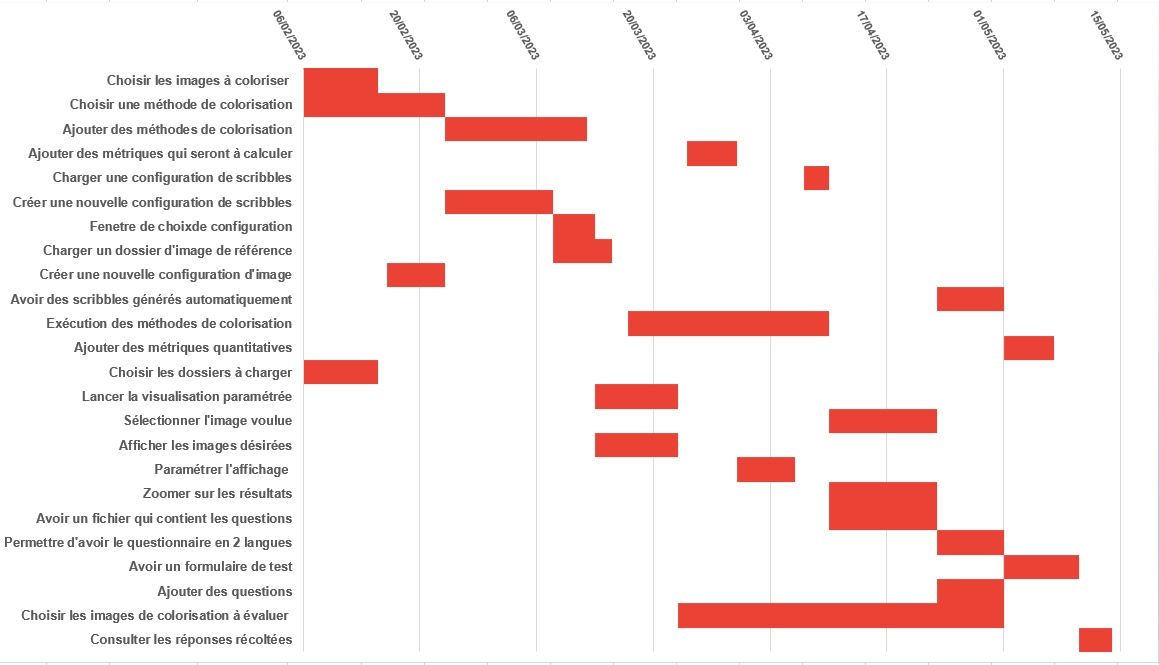
\includegraphics[width=15cm]{gantt.png}
    \caption{Planification des tâches à l'aide d'un diagramme de gantt}
    \label{fig:gantt}
\end{figure}

Cependant, même si ce diagramme est utile pour représenter le déroulement total du projet, il ne doit pas rentrer en contradiction avec les méthodes agiles.
Il pourra servir de support mais nous ne devrons pas essayer de le suivre parfaitement et privilégier les méthodes agiles
en prenant en compte des éventuels changements.

\subsection{Risques et actions}\label{sec:risques}

Plusieurs risques sont à prévoir quant au bon déroulement du projet. Tout d'abord, le premier risque est lié
à la planification du projet. En effet, nous avons essayé de faire une analyse fonctionnelle des besoins du client et ensuite
de faire une liste de tâches associées à chacun des besoins. Pour chacune de ces tâches, nous avons estimé le temps nécessaire pour la réaliser.
Ce temps est utilisé pour planifier le déroulement du projet, notamment l'ordre de réalisation de chacune des tâches.
Le risque est ici que l'estimation du temps nécessaire à chaque tâche soit erronée (notamment sous-estimée) et que cela entraîne donc des perturbations
dans le planning du projet ou un surmenage de certains membres de l'équipe afin de finir les tâches dans les temps.

Des mauvais choix techniques sont aussi à envisager. En effet, nous avons fait des choix techniques dans les technologies que nous allons utiliser
mais aussi, dans l'architecture du code que nous avons imaginée. Cette architecture a pour but de nous faciliter le codage par la suite, en s'assurant 
que tout les membres de l'équipe aient une vision globale du projet. Changer des choix techniques que nous avons fait peut avoir beaucoup de conséquences
et être très couteux en temps.

Afin de minimiser ces deux risques, nous avons choisi de commencer l'implémentation assez tôt dans le projet. Cela nous permet de mesurer concrètement le temps que peuvent
prendre certaines tâches et donc de ré-évaluer le temps estimé pour les autres en fonction. Cela permet également de confirmer que les technologies que nous utilisons sont adaptées 
pour répondre aux besoins du projet.

Un des autres risques du projet est de ne pas avoir cerné toutes les exigences du client lors de la première phase et 
de découvrir des besoins importants tard dans le projet. Les besoins du client ont été étudiés pendant presque 2 mois
pendant lesquels nous avons pu en discuter par l'intermédiaire de plusieurs réunions. Lors de ces réunions, des propositions
d'interfaces, des listes de besoins ainsi que l'architecture du projet ont été discutés afin de cerner au mieux ses besoins fonctionnels.
Cependant, il est malgré tout possible que certains aspects n'aient pas été abordés lors de ces discussions et soient découverts 
lors de futures réunions et démonstrations. Cela est un risque car plus une exigence est découverte tard dans le projet,
plus elle "coûte cher", c'est-à-dire plus elle prendra de temps à être implémentée. En effet, cela impliquera peut-être de changer
des éléments du projets, ce qui pourrait être évité en découvrant l'exigence plus tôt.

De plus, il est également possible que nous ayons oublié des dépendances entre certaines tâches et que nous nous en rendions compte lors de 
la phase d'implémentation du projet. Cela impliquerait de devoir changer l'organisation et les prévisions que nous avons fait.

Concevoir ce projet de manière agile est l'une des manières de minimiser ces risques. En effet, comme nous l'avons dit dans des sections précédentes, conduire un projet en suivant une méthodologie
agile consiste à réaliser des courtes itérations qui sont limitées dans le temps et qui contiennent des objectifs à réaliser. À la fin de chaque itération,
des démonstrations faites pour le client afin de lui montrer ce qui a été réalisé. Ces réunions fréquentes permettent donc de faire le point régulièrement avec le client sur 
ses besoins et de prendre en compte rapidement des éventuels changements.

Il faut aussi s'assurer qu'il n'y ait pas de mauvaise coordination entre les membres de l'équipe et que certaines parties du projet qui sont réalisées
séparement ne soient pas compatibles lorsque l'on cherche à les assembler. Une des actions à prévoir pour pallier à ce problème est de définir des réunions fréquentes
qui permettent à toute l'équipe de se retrouver, de discuter du projet et de son avancement. Dans les projets agiles classiques, ces réunions prennent la forme de 
\textit{daily scrum} lors desquels l'équipe se retrouve tous les jours pendant une quinzaine de minutes. Cependant, notre contexte de travail de ce projet, notamment des emplois
du temps différents, rendent les \textit{daily scrum} difficiles à réaliser. Pour ce projet, il est plus réaliste que l'équipe ne se retrouve pas tous les jours mais plutôt tous les
quelques jours (tous les 3 ou 4 jours par exemple) pour des réunions courtes afin de se coordonner sur les différents modules.

Enfin, un des autres risques est d'avoir une mauvaise gestion du temps consacré à ce projet par rapport aux autres obligations que nous avons,
comme les cours ou les autres projets.  Pour anticiper ce problème, il est nécessaire de prévoir un nombre d'heures hebdomadaire qui seront consacrées à ce projet.
Ce nombre d'heures doit être réaliste, c'est-à-dire qu'il ne doit pas excéder les capacités de chacun des membres de l'équipe.
Il doit également être à peut près constant tout au long du projet, pour éviter des phases déséquilibrées où le projet n'avance plus ou beaucoup moins rapidement.
Il est donc possible de prévoir que chacun des membres de l'équipe travaille quelques heures par semaine sur ce projet.
En plus d'organiser un nombre d'heure de travail fixe par semaine et par personne, il est également possible d'envisager des créneaux de travail fixes
chaque semaine, intégrés à l'emploi du temps, pour que chacun ait ce projet dans son planning de manière fixe.


\section{Premières réalisations}

Les réalisations permettent de transformer le projet d'un projet conceptuel en quelque chose de concret.
Plusieurs réalisations ont été faites quant au projet. Tout d'abord, nous avons réalisé des maquettes, afin d'analyser
les besoins fonctionnels en suivant une approche \textit{design first}. Elles se trouvent dans la section \ref{sec:maquette}.
De plus, afin de s'intégrer dans une démarche agile et de réaliser de meilleurs estimations, nous avons commencé l'implémentation
du projet. La description des fonctionnalités que nous avons déjà implémentées se trouve en section \ref{implementation-code}.

\subsection{Maquettes de l'interface graphique}\label{sec:maquette}

Afin de concrétiser les besoins du client et de les valider, des maquettes de l'interface graphique ont été réalisées.
Les maquettes ont été volontairement créées de manière simple, c'est-à-dire que le choix des couleurs n'est pas pris en compte
ni le design spécifique à chaque partie de l'interface.
L'essentiel avec ces maquettes, était d'imaginer comment tous les besoins du client pouvaient être satisfait
et d'en discuter facilement avec lui pour voir si cela correspondait à ce qu'il attendait. Dans cette partie, seules les maquettes principales sont présentées.
L'ensemble des maquettes se trouve dans la section \ref{sec:annexe-maquette} des annexes.
Ces maquettes ont été créées à l'aide du logiciel \href{https://www.figma.com/}{figma} qui permet de réaliser des maquettes de manière collaborative.

Dans cette partie, certaines maquettes réalisées seront présentées et décrites afin de comprendre comment
elles permettent de répondre aux besoins du client. 

Tout d'abord, plusieurs maquettes ont été réalisées pour la partie colorisation.

\begin{figure}[!ht]
    \centering
    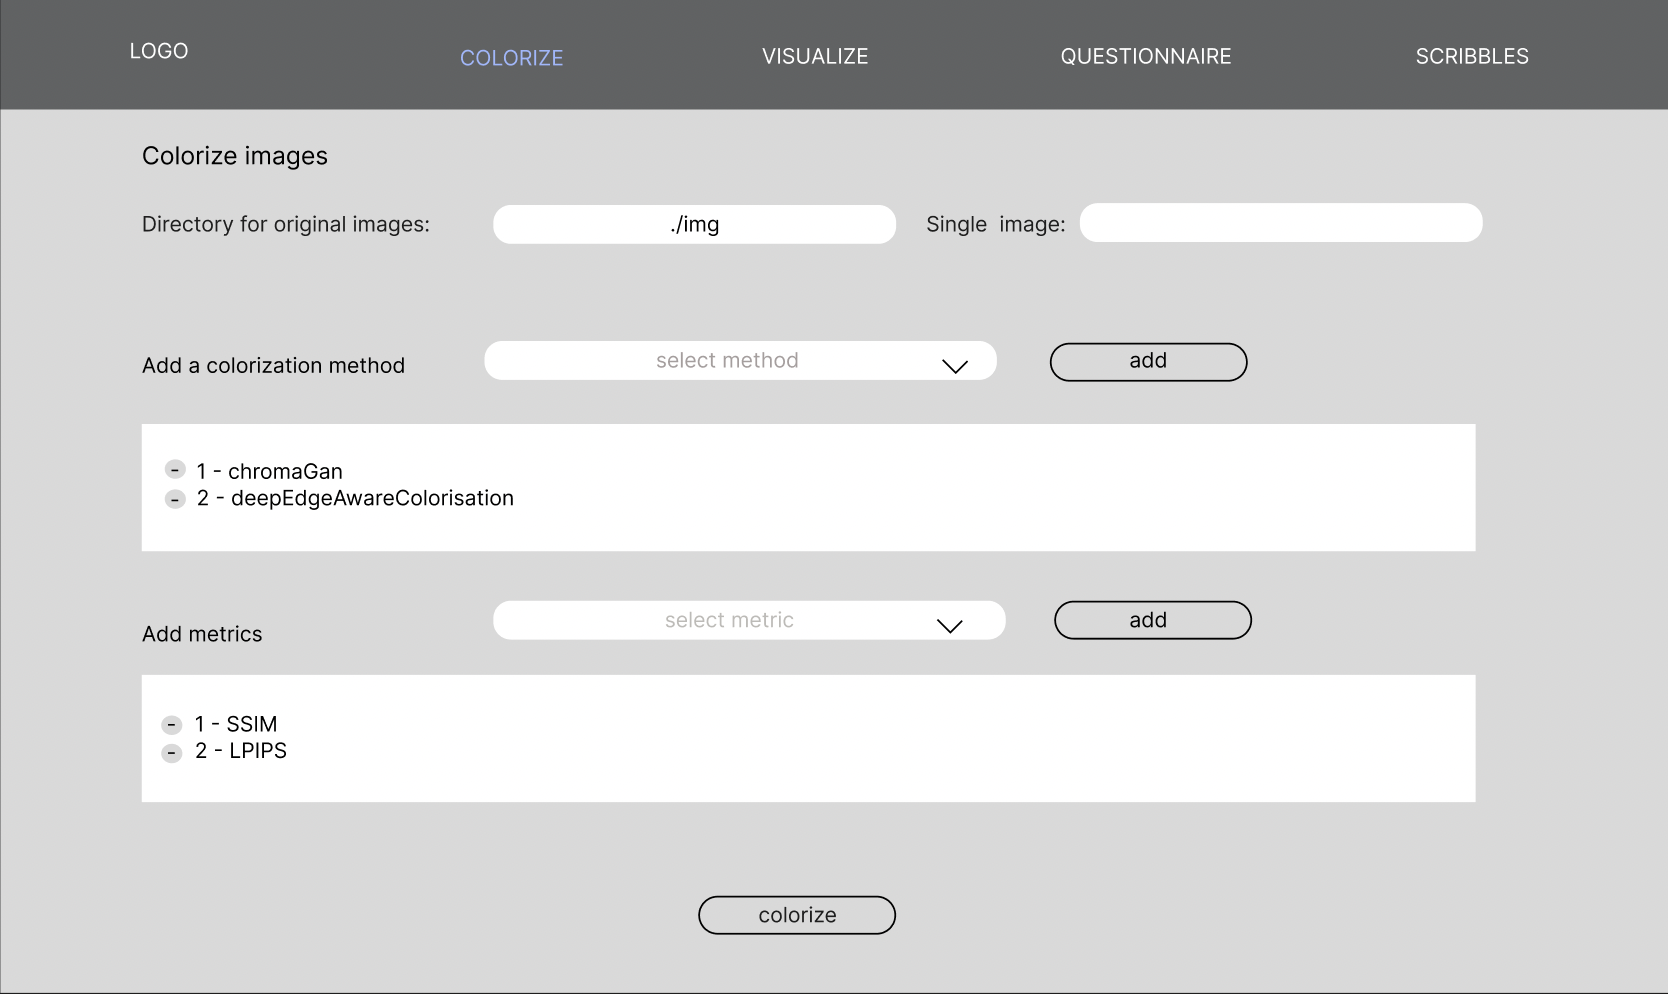
\includegraphics[width=11cm]{coloriser-parametrage1.png}
    \caption{Maquette : paramétrer la colorisation}
    \label{fig:coloriser-parametrage1}
\end{figure}

La figure \ref{fig:coloriser-parametrage1} représente l'interface qui permettrait de paramétrer la colorisation avant de la lancer.
Sur cette interface, plusieurs champs sont disponibles. Premièrement, il y a un champ permettant de renseigner le dossier d'images en noir et blanc
que l'on souhaite coloriser (pour faire de faire de la colorisation par \textit{batch}) ou un champ permettant de choisir directement une image (pour coloriser une seule image). Ensuite, un deuxième champ permet d'ajouter des méthodes de colorisation. Ces méthodes peuvent être sélectionnées
à l'aide d'un menu déroulant et ajoutées à la liste située en dessous avec le bouton \textit{add}.
La liste des méthodes affichées dans le carré blanc représente donc toutes les méthodes qui seront exécutées sur le dossier d'images choisi.
Il est également possible de supprimer des méthodes de cette liste à l'aide du bouton \textit{-}.
Le même principe est appliqué pour les métriques. La liste des métriques représente celles qui seront calculées lors de la colorisation.
Le bouton \textit{colorize} permet de lancer la colorisation.

De plus, si l'une des méthodes ajoutées nécessite des scribbles, alors une fenêtre \textit{pop-up} apparaît
afin de permettre à l'utilisateur de paramétrer les scribbles. Il peut alors charger une configuration de scribbles déjà définie (c'est-à-dire
un ensemble de scribbles dans un dossier qui correspondent au dossier d'images sélectionné) ou en créer une nouvelle.
Un processus similaire est imaginé pour les méthodes de colorisation nécessitant des images par référence.

Ainsi, s'il choisit de créer une nouvelle configuration de scribbles, l'interface présentée en figure \ref{fig:coloriser-scribbles} est affichée.

\begin{figure}[!ht]
    \centering
    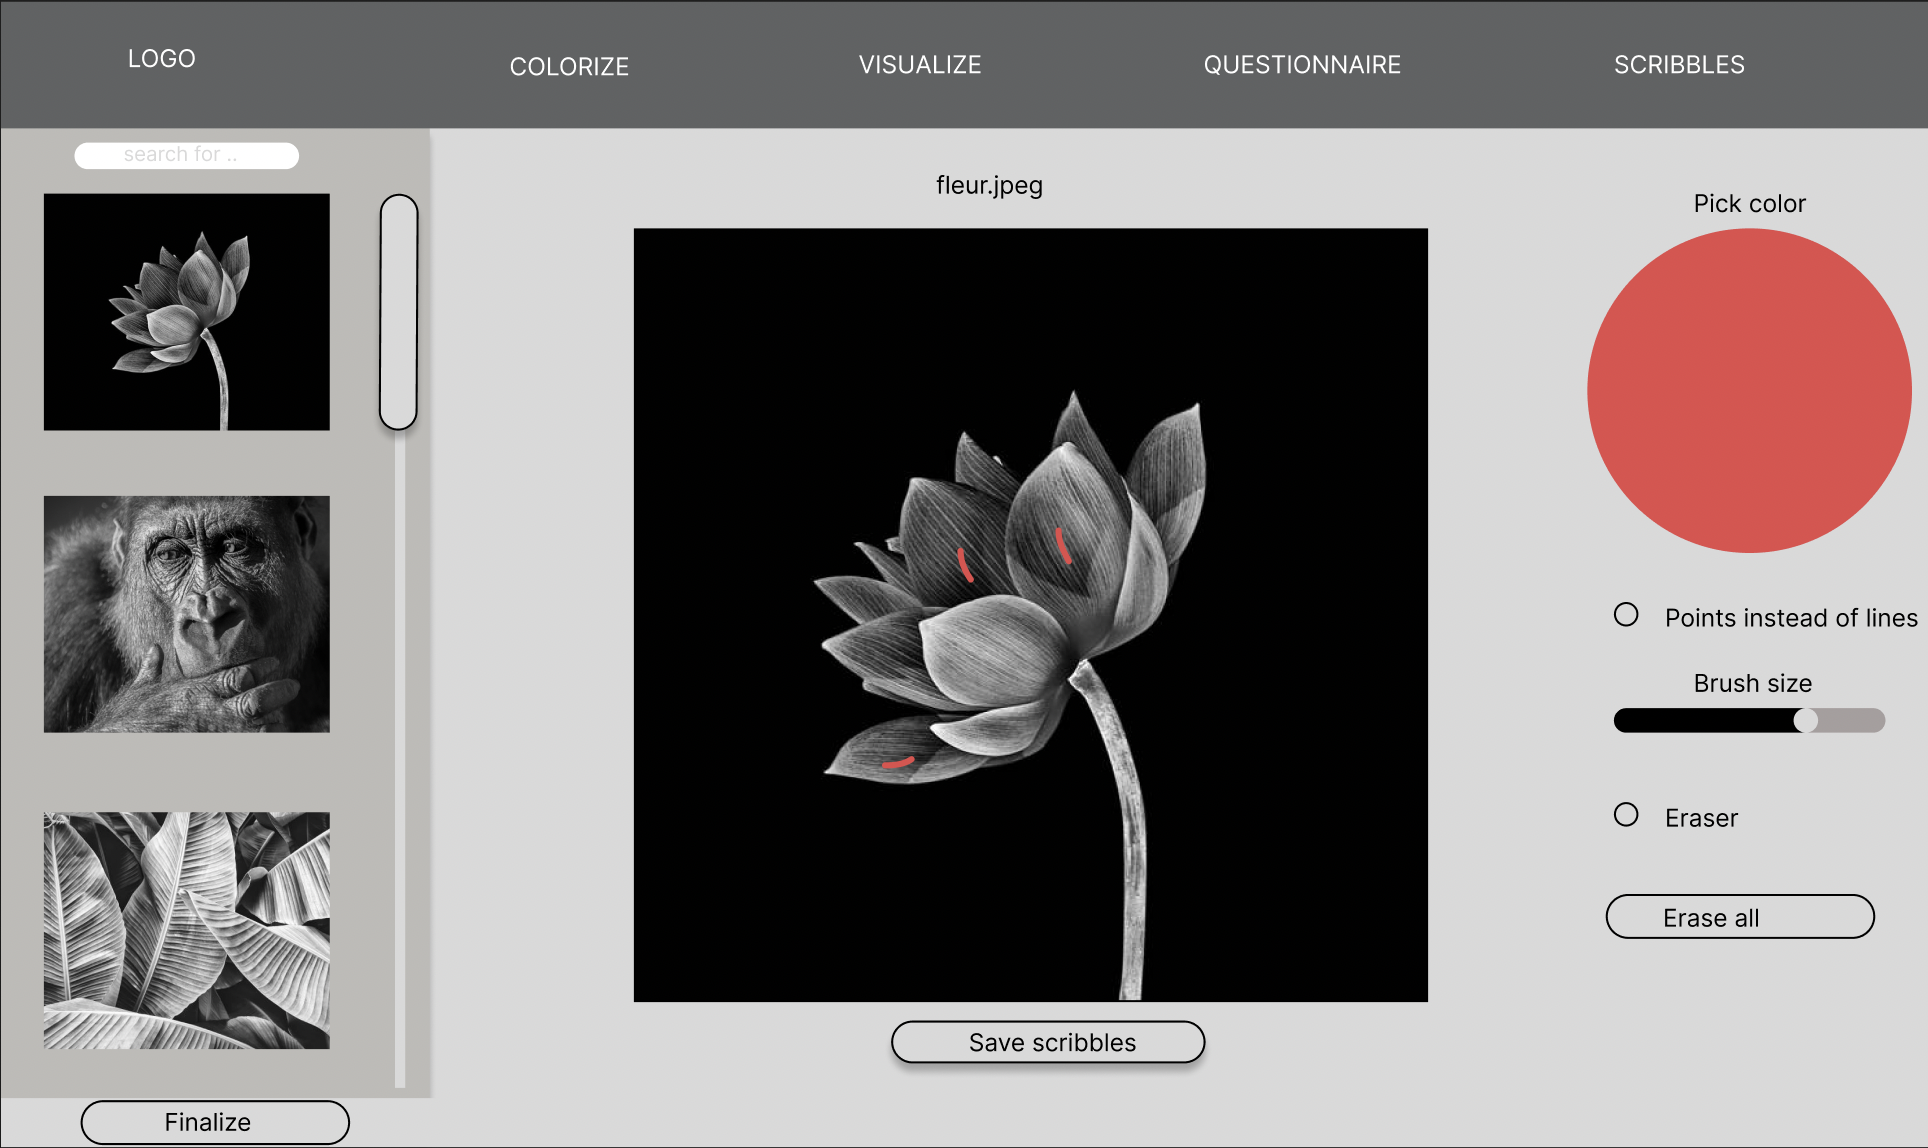
\includegraphics[width=11cm]{coloriser-scribbles.png}
    \caption{Maquette : créer des scribbles}
    \label{fig:coloriser-scribbles}
\end{figure}

À gauche, il y a une barre déroulante avec la liste des images du dossier en question. Une barre de recherche est également disponible pour
pouvoir trouver une image rapidement par son nom.
En cliquant sur une des images de cette liste, elle s'affiche sur la partie droite de l'écran avec son nom.
À droite de l'image des outils permettant de réaliser les scribbles sont présents. Ainsi, il y a un \textit{sélectionneur} qui permet de choisir la
couleur du pinceau. La jauge annotée \textit{Brush size} permet de régler la taille du pinceau.
Le bouton \textit{Points instead of lines} fait que les scribbles ne seront plus des traits mais des points d'un pixel puisque certaines 
méthodes de colorisation prennent seulement des points de couleur. Sur l'interface, il est également prévu des outils permettant d'effacer les scribbles. Ainsi,
lorsque le bouton \textit{Eraser} est coché, le pinceau n'écrira plus de scribbles sur l'image mais les effacera. Le bouton \textit{Erase all} efface tous les scribbles qui ont été 
dessinés auparavant.
Enfin, le bouton \textit{Save scribbles} permet de sauvegarder le scribble et le bouton \textit{Finalize} enregistre la configuration une fois que tous les scribbles ont été 
créés dans un dossier en suivant l'architecture définie.

Une fois que la colorisation paramétrée (avec les éventuels scribbles ou images de références) et lancée se finit, une interface représentée en figure \ref{fig:coloriser-succes} avec 
des informations s'affiche.

\begin{figure}[!ht]
    \centering
    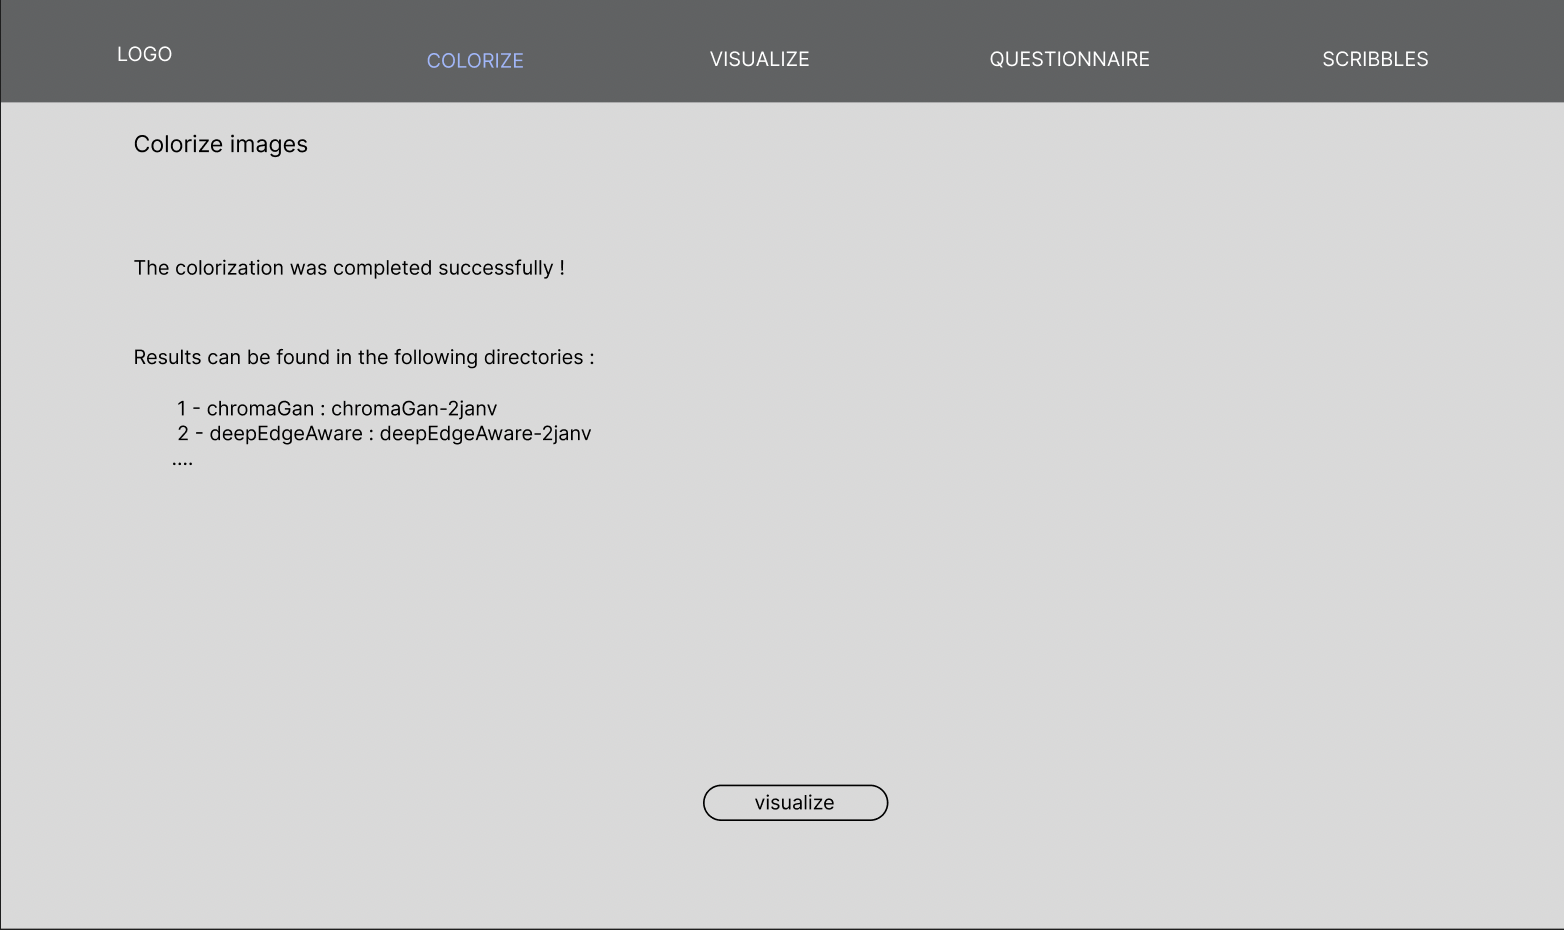
\includegraphics[width=11cm]{coloriser-succes.png}
    \caption{Maquette : une fois la colorisation réussie}
    \label{fig:coloriser-succes}
\end{figure}

Cet écran contient des informations sur les colorisations qui viennent d'être effectuées (par exemple le nom des dossiers où les images ont été sauvegardées).
Le bouton \textit{Visualize} permet de se rendre directement à l'écran de la figure \ref{fig:visualiser-comparaison3} pour voir les résultats.
%% menu pour les scribbles

De plus, des interfaces ont également été imaginées pour la partie permettant de visualiser des résultats de colorisation.
Ainsi, de même que pour la colorisation, un premier écran illustré en figure \ref{fig:visualiser-choix} permet de paramétrer la visualisation qui sera effectuée.

\begin{figure}[!ht]
    \centering
    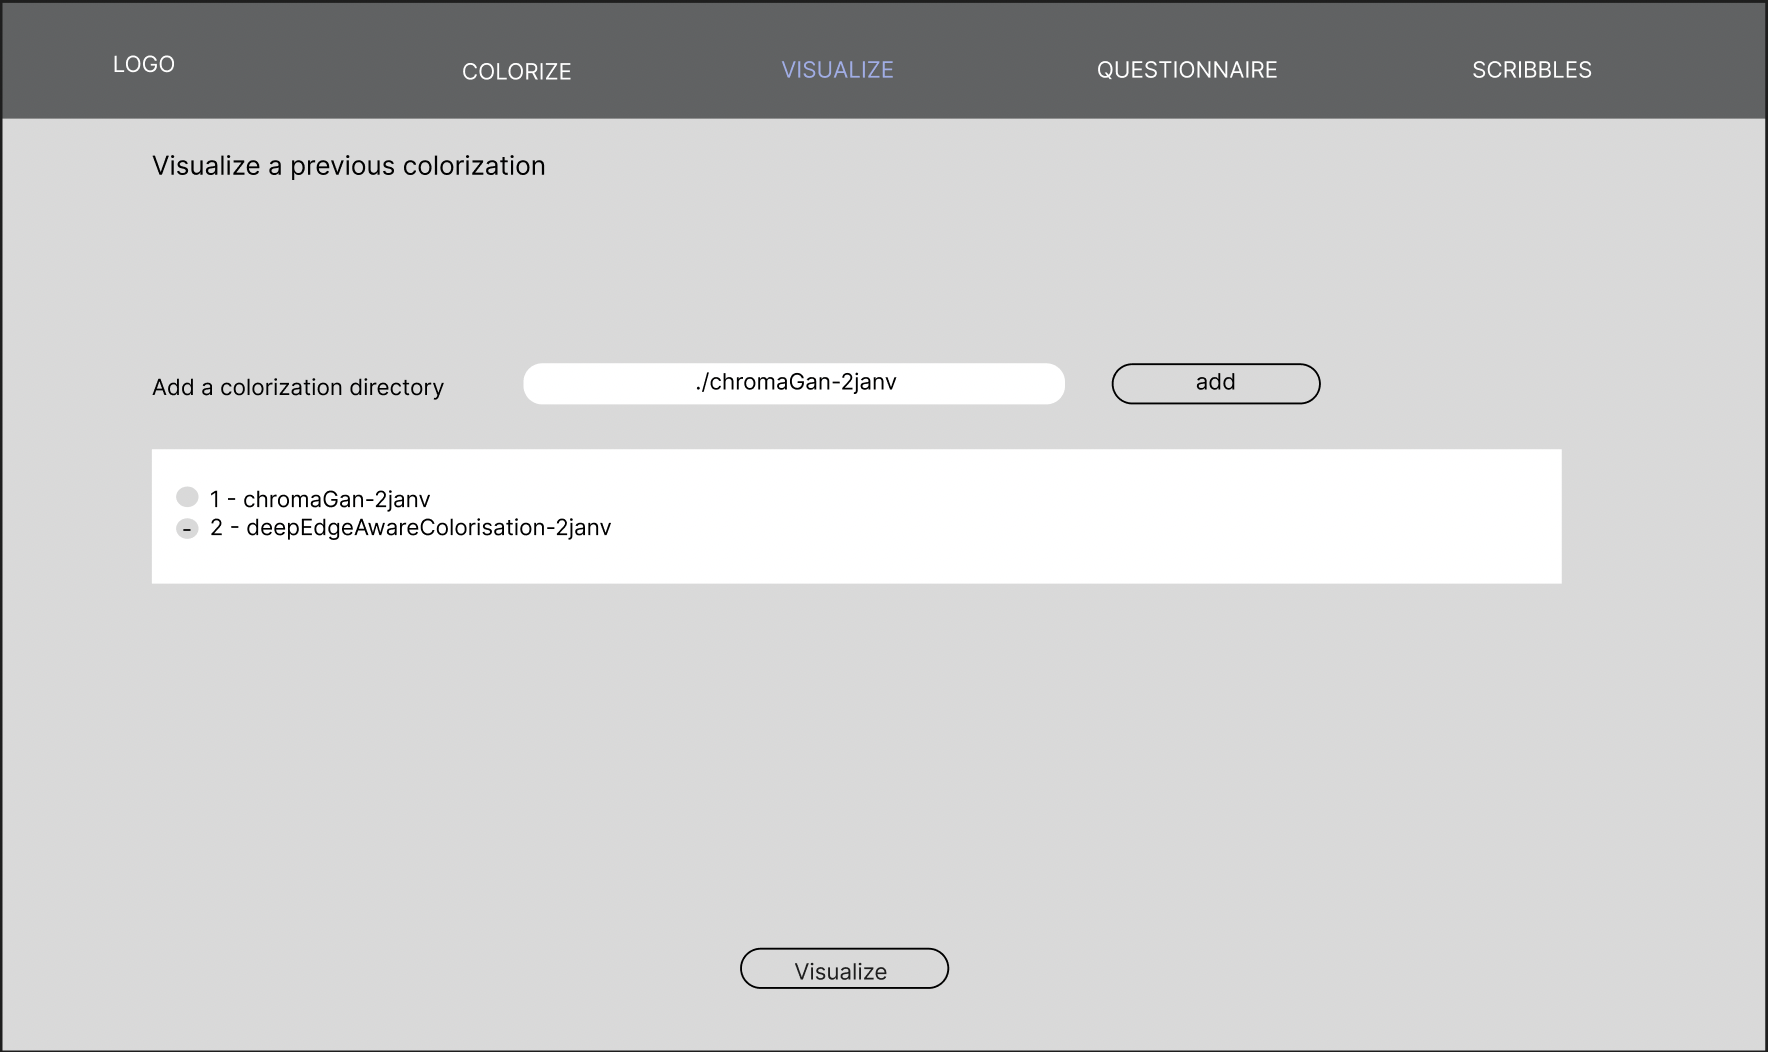
\includegraphics[width=11cm]{visualiser-choix.png}
    \caption{Maquette : paramétrer une visualisation}
    \label{fig:visualiser-choix}
\end{figure}

Dans cette interface, il s'agit seulement de sélectionner les dossiers qui contiennent les résultats des colorisations que l'on souhaite visualiser.
L'utilisateur n'a pas à renseigner le dossier des images en noir et blanc d'origine ni les images \textit{groundtruth}, le lien se fait automatiquement.
Cela se déroule de la même manière pour les métriques, les métriques qui seront affichées seront les métriques calculées lors de la colorisation. Lors de cette étape, il faudra donc bien
vérifier que les dossiers des images que l'on souhaite visualiser concernent donc bien les mêmes images d'origine.
Le bouton \textit{Visualize} permet de visualiser la colorisation en passant à l'interface représentée dans la figure \ref{fig:visualiser-comparaison3}.

\begin{figure}[!ht]
    \centering
    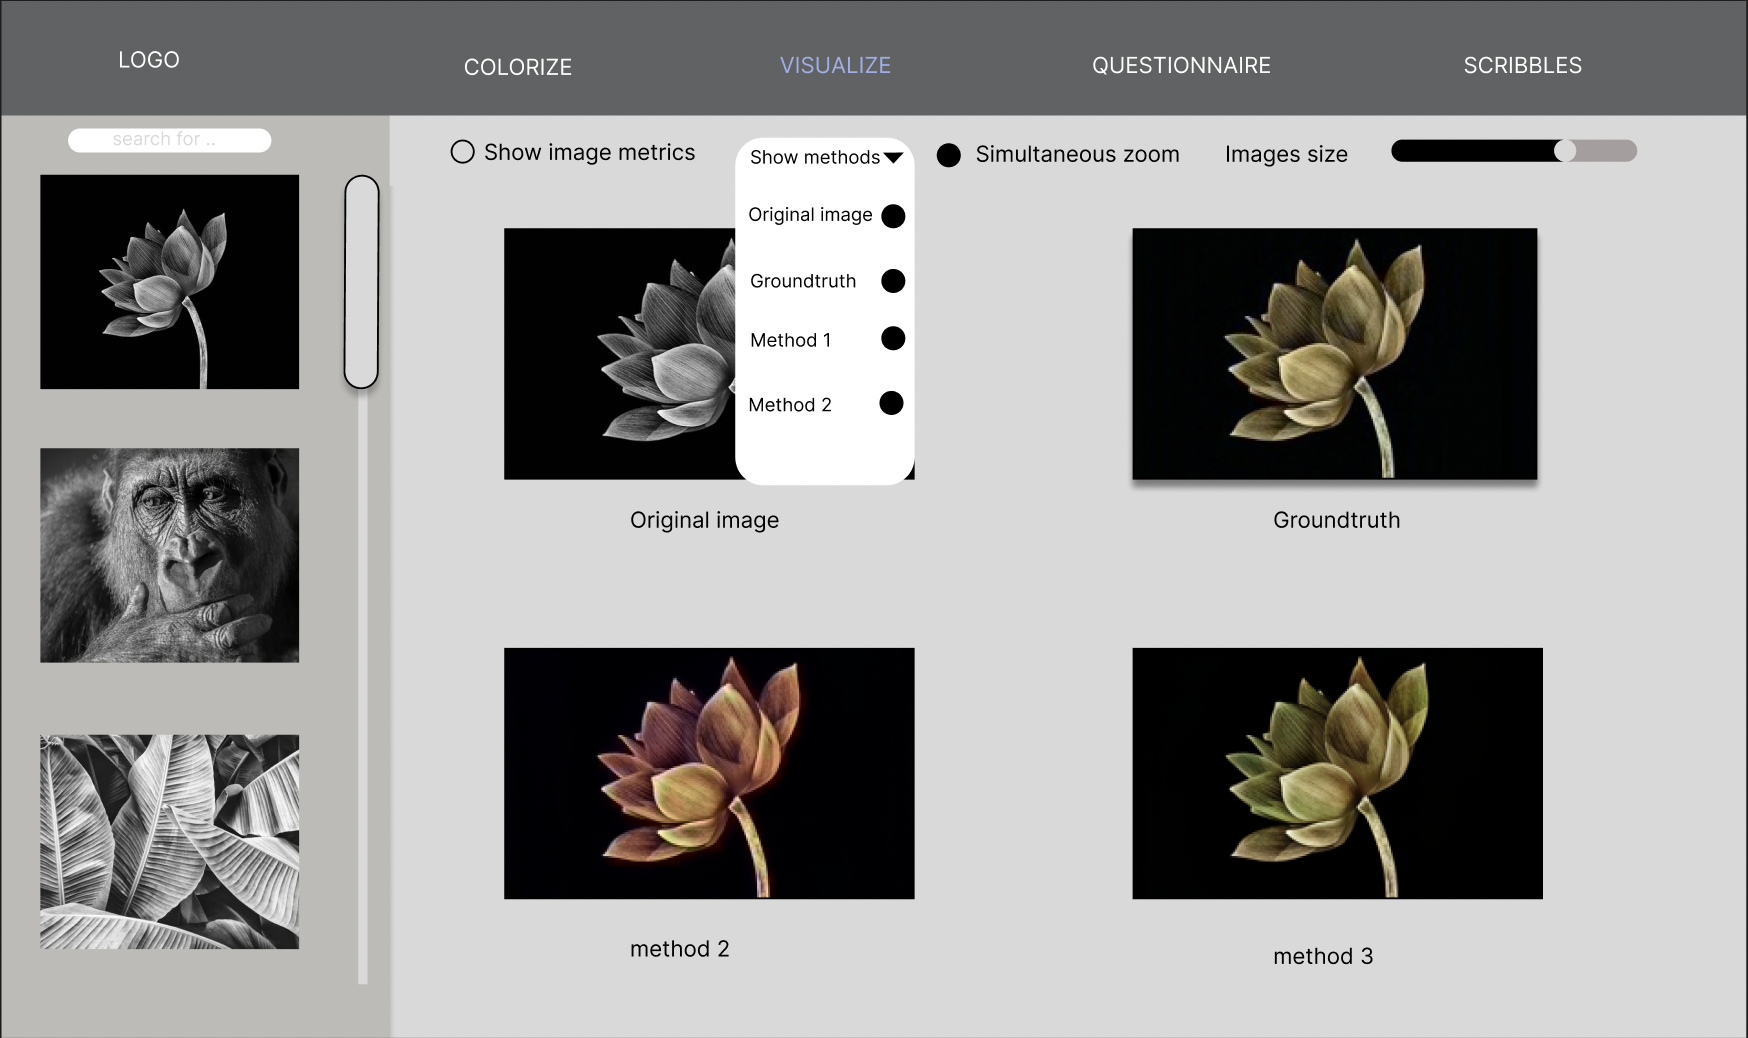
\includegraphics[width=11cm]{visualiser-comparaison3.png}
    \caption{Maquette : visualiser un résultat de colorisation}
    \label{fig:visualiser-comparaison3}
\end{figure}

Comme pour les scribbles, une section avec une barre déroulante et une barre de recherche permet d'accéder à toutes les images du dossier.
Une fois l'image sélectionnée, plusieurs images vont alors s'afficher à l'écran : l'image d'origine en noir et blanc, l'image \textit{groundtruth}
d'origine en couleur si elle existe ainsi que les mêmes images issues des différentes colorisations sélectionnées.
La jauge \textit{Images size} en haut à droite de l'écran permet d'agrandir ou de réduire la taille des images affichées.
Le nombre d'images qui sont visibles sur le même écran dépend donc de leur taille et ce curseur permet donc d'augmenter ou de réduire le nombre d'images apparaissant côte à côte.
Si toutes les images ne peuvent pas être affichées sur le même écran à une certaine taille, alors il faudra descendre pour toutes les visualiser.
Le bouton \textit{Image metrics} permet d'afficher les métriques sélectionnées en dessous de chacune des images.
Enfin, la barre déroulante \textit{Show methods} permet de cocher ou de décocher les images que l'on souhaite afficher à l'écran.
L'effet de zoom s'effectuera tel un effet loupe sur la souris lorsque cette dernière survole l'une des images affichées. Il s'effectuera sur toutes les images simultanément à condition que 
le bouton \textit{Simultaneous zoom} soit coché.

Enfin, plusieurs maquettes ont été créées pour les questionnaires. La partie des questionnaires est vaste car il faut pouvoir créer un questionnaire
depuis l'interface, répondre à un questionnaire et également visualiser les réponses qui auront été enregistrées.
Premièrement, la figure \ref{fig:questionnaire-creation} illustre l'interface qui permet de créer un questionnaire.

\begin{figure}[!ht]
    \centering
    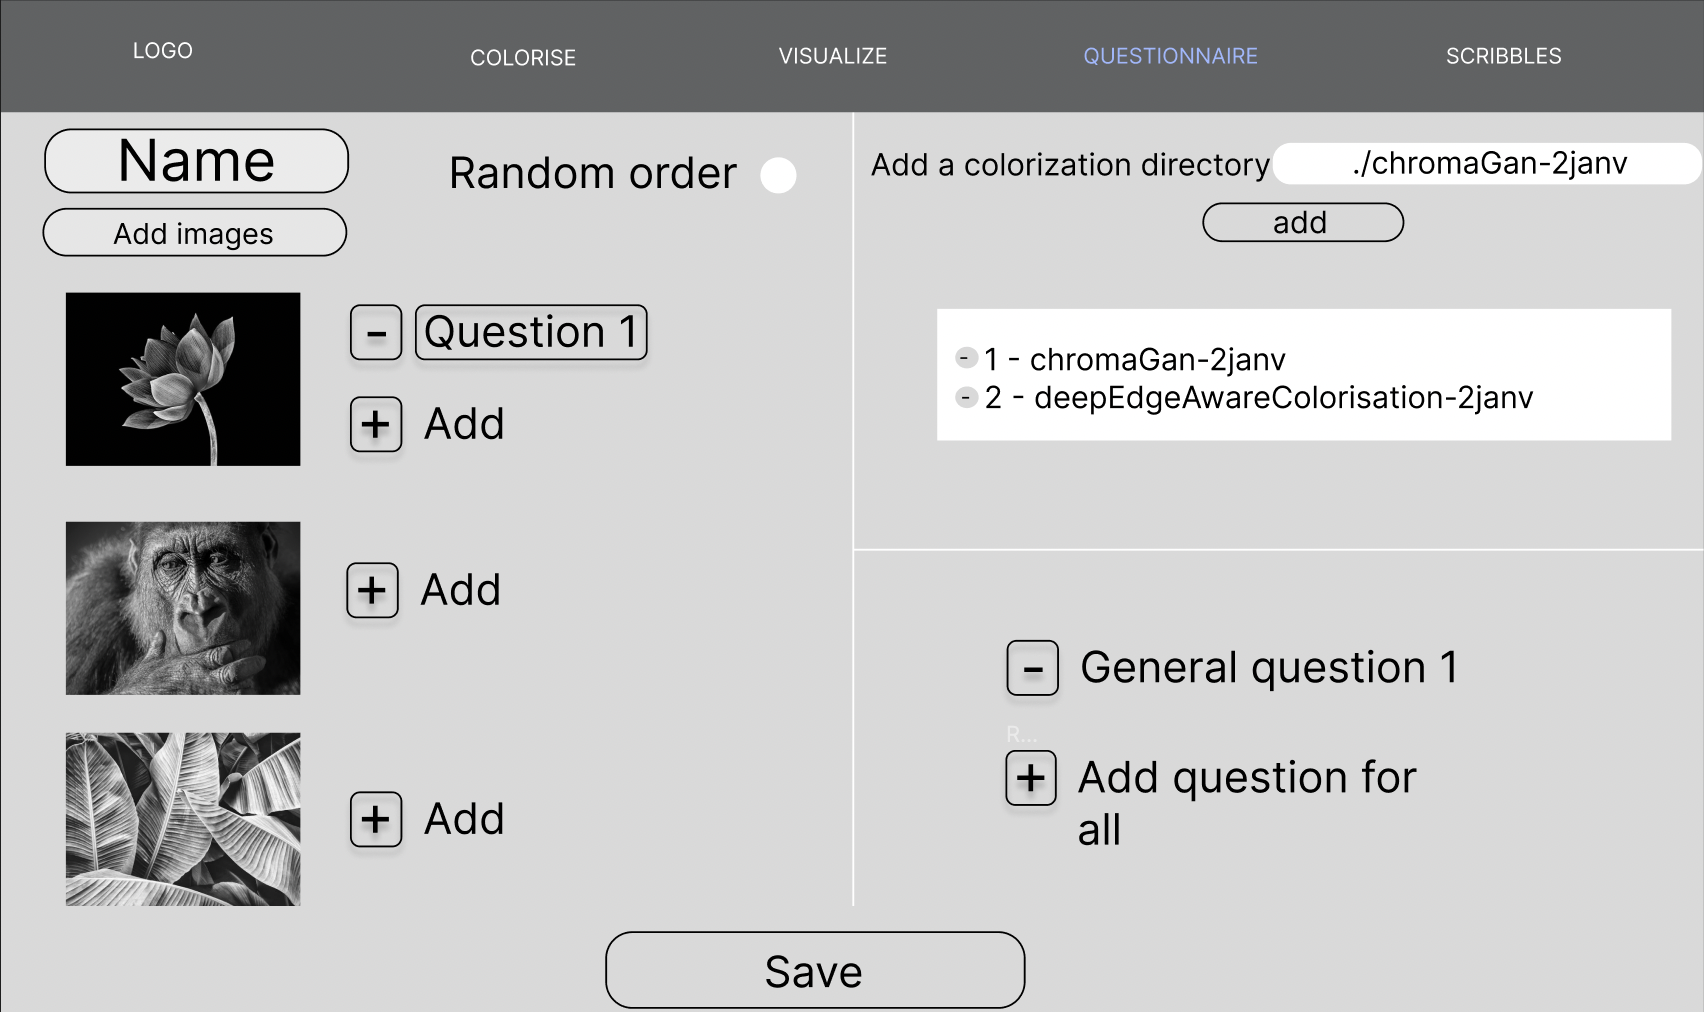
\includegraphics[width=11cm]{questionnaire-creation.png}
    \caption{Maquette : créer un questionnaire}
    \label{fig:questionnaire-creation}
\end{figure}

Le champ \textit{Name} permet de choisir un nom pour le questionnaire. Le champ \textit{Add Images} permet d'ajouter
des images qui apparaitront dans le questionnaire. En dessous de ce bouton, les images qui ont été sélectionnées apparaissent.
À côté de ces images, il y a un bouton \textit{+} qui apparait et qui permet d'ajouter des questions qui seront posées sur cette image.
Lorsque l'on a décidé d'ajouter une question pour une image, l'écran présenté en figure \ref{fig:questionnaire-creation-question2} s'affiche afin de configurer la question. Une fois cela effectué,
elle s'affiche à côté comme pour \textit{Question 1} et il est possible de la supprimer à l'aide
du bouton \textit{-}.
Cette interface prend également en compte des questions qui peuvent apparaître pour toutes les images choisies. Ces questions apparaissent à droite de l'écran.
De même, il est possible d'en ajouter ou d'en supprimer à l'aide des bouton \textit{+} et \textit{-}.
Un bouton à cocher \textit{Random order} permet de choisir si les questions de ce questionnaires apparaîtront dans un ordre aléatoire. Enfin, comme pour paramétrer une visualisation,
il est possible d'ajouter les colorisations dont on souhaite que les images apparaissent dans les questions. 
Le bouton \textit{Save} permet de sauvegarder ces paramètres et de passer à l'écran suivant décrit par la figure \ref{fig:questionnaire-creation-question1}.

\begin{figure}[!ht]
    \centering
    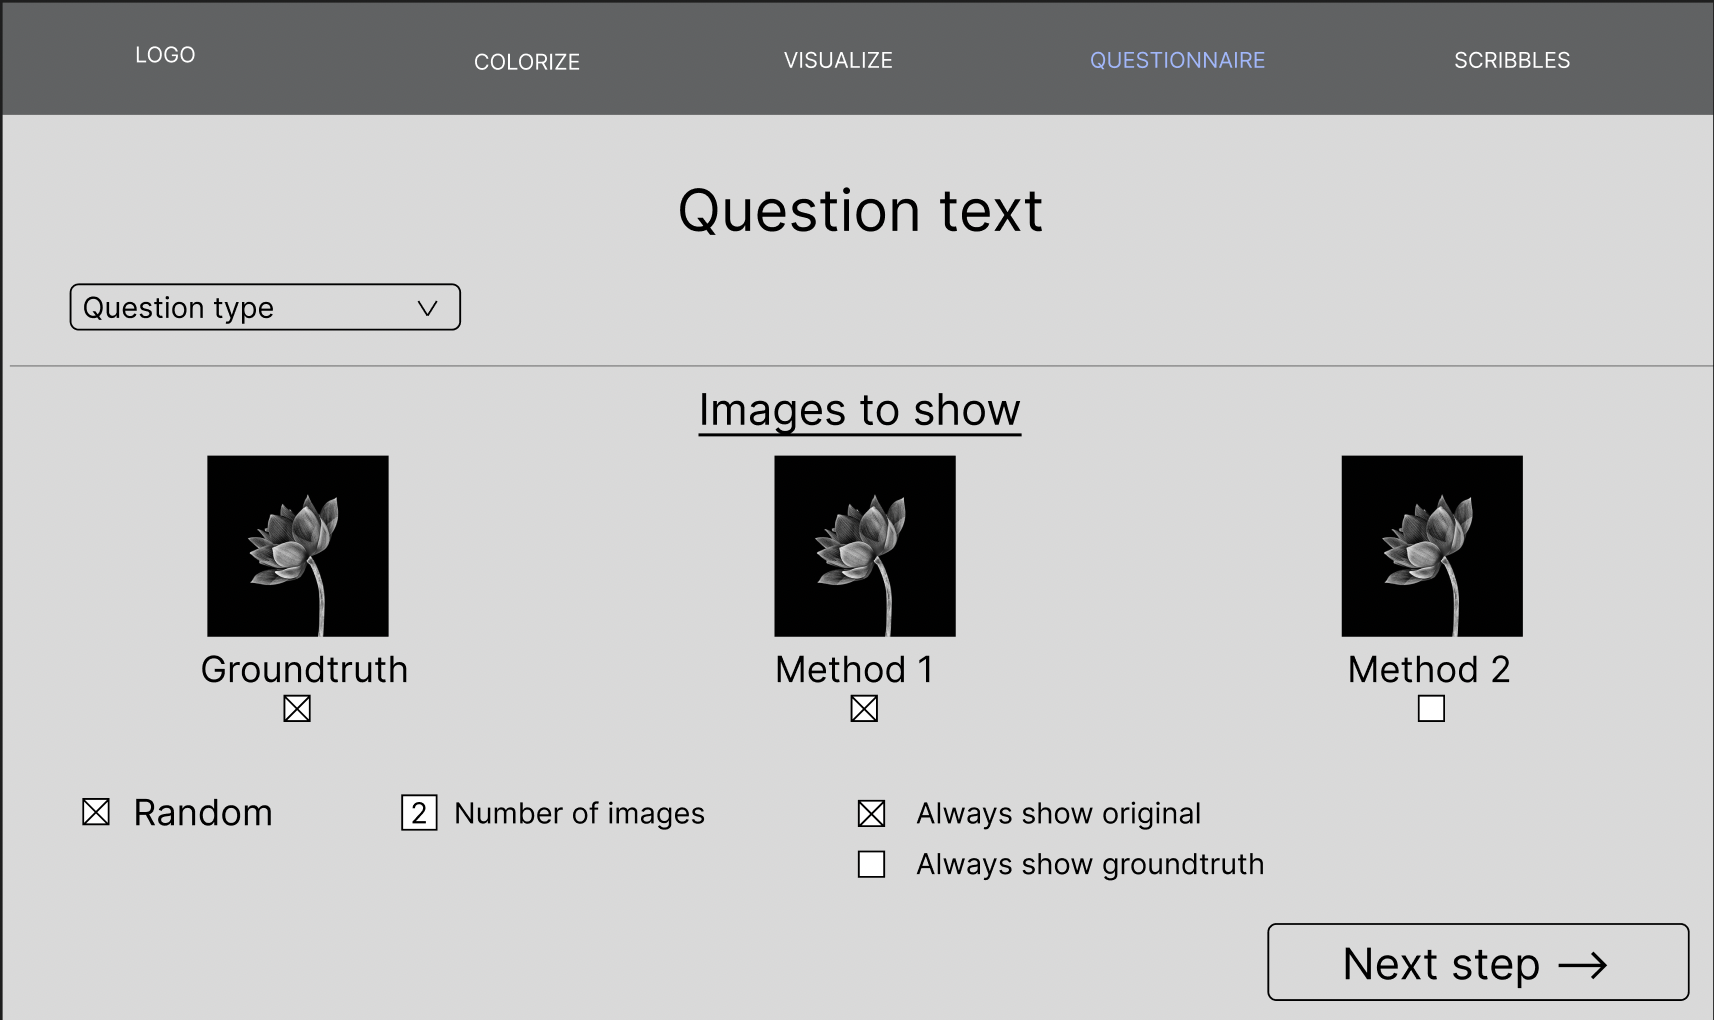
\includegraphics[width=11cm]{questionnaire-creation-question1.png}
    \caption{Maquette : créer une question}
    \label{fig:questionnaire-creation-question1}
\end{figure}

Ainsi, lorsqu'une question est créée, il est possible de la paramétrer de différentes manières.
Le champ \textit{Question text} permet donc d'ajouter le texte de la question. Il est possible de choisir le type de la question (par exemple un classement 
de méthodes ou une question plus libre sur des aspects de l'image avec du texte) que l'on est en train
Enfin, la partie basse de l'écran permet de cocher et de décocher les images qui seront affichées à l'écran ainsi que d'autres paramètres d'affichage.
de paramétrer à l'aide du menu déroulant \textit{Question type} juste en dessous. Celui-ci permet de pré-remplir les champs selon certains archétypes de question renseignés dans le logiciel.
Cependant, à ce stade, le paramétrage d'une question n'est pas finalisé et le bouton \textit{Next step} dirige vers le deuxième écran (figure \ref{fig:questionnaire-creation-question2}) qui permet de paramétrer une question.

\begin{figure}[!ht]
    \centering
    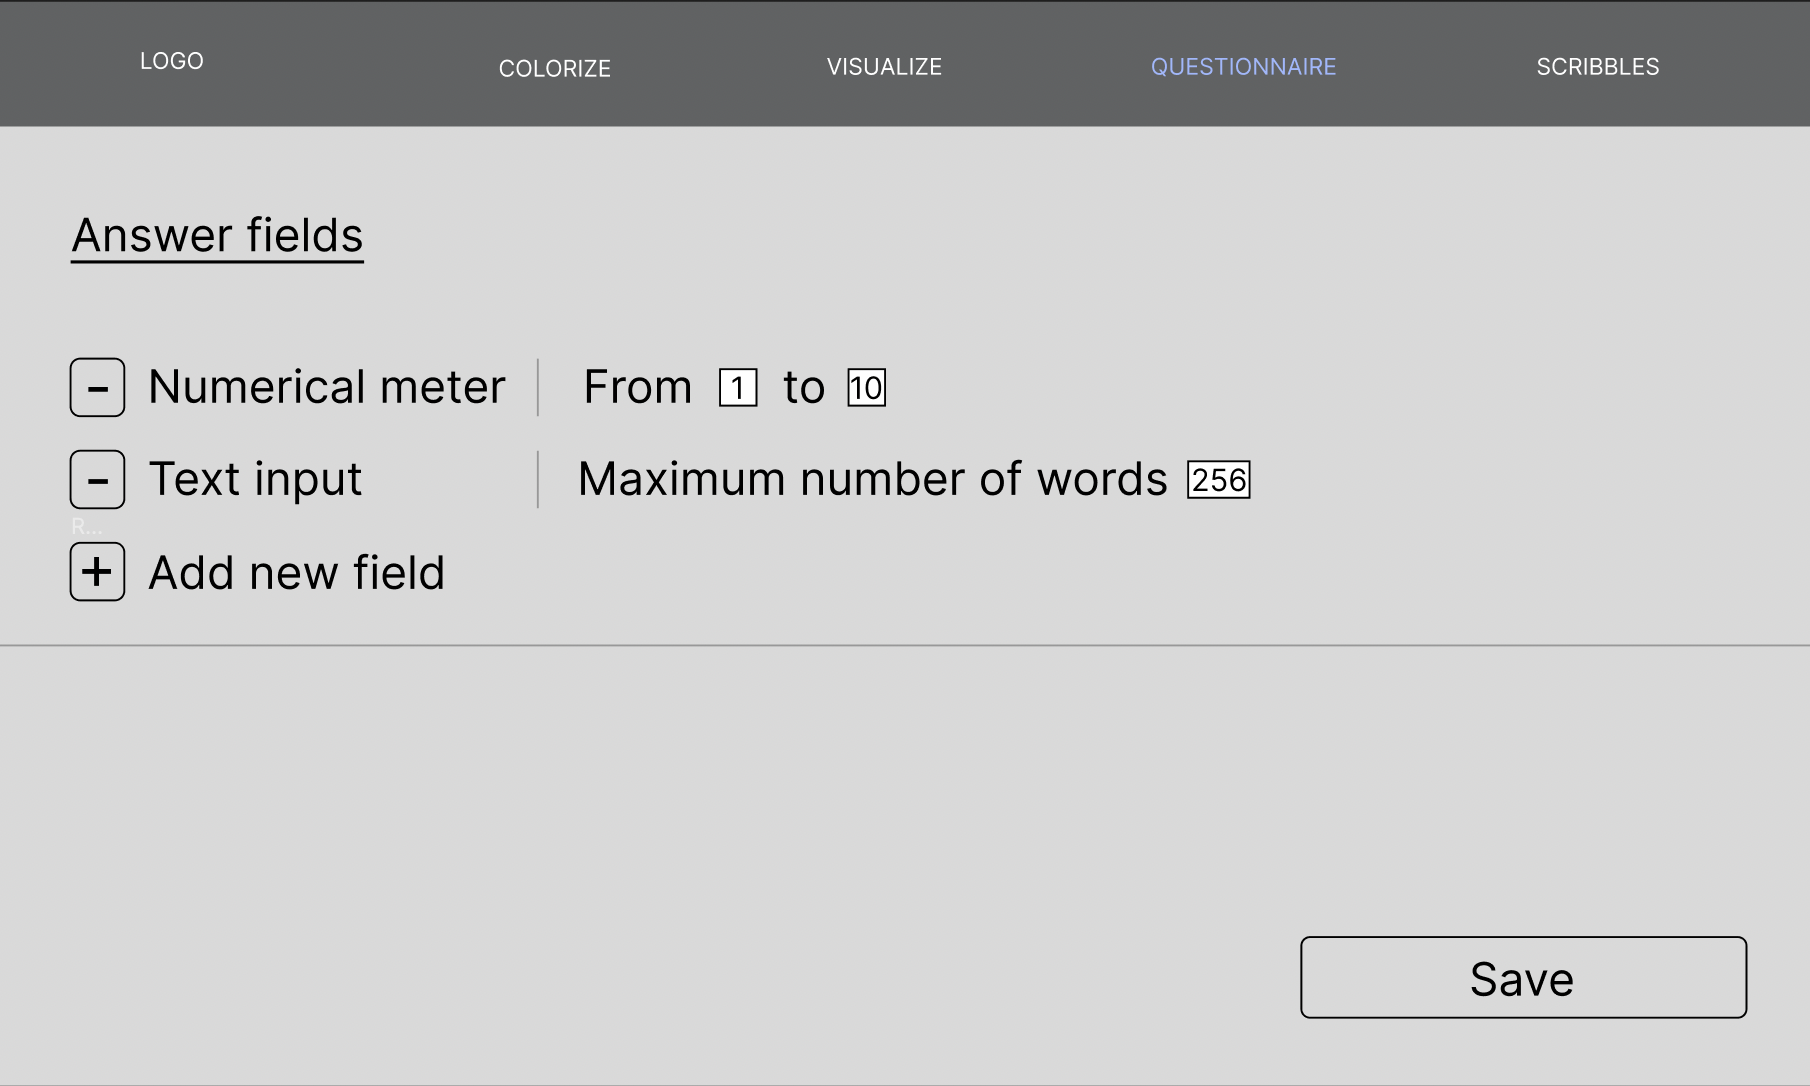
\includegraphics[width=11cm]{questionnaire-creation-question2.png}
    \caption{Maquette : créer une question (bis)}
    \label{fig:questionnaire-creation-question2}
\end{figure}

Cette interface permet d'ajouter ou de supprimer des champs de réponse pour la question.
Une nouvelle fois, les boutons \textit{+} et \textit{-} permettent d'ajouter ou de supprimer un nouveau champ.
À droite, il est possible de paramétrer le champ de réponse en fonction de son type (par exemple, si l'on attend un champ de texte, 
il est possible de limiter le nombre de caractères). Enfin, le bouton \textit{Save} permet de sauvegarder la question et ses contraintes.

Une maquette a également été créée pour répondre aux questions. La figure \ref{fig:questionnaire-repondre} illustre cette interface.

\begin{figure}[!ht]
    \centering
    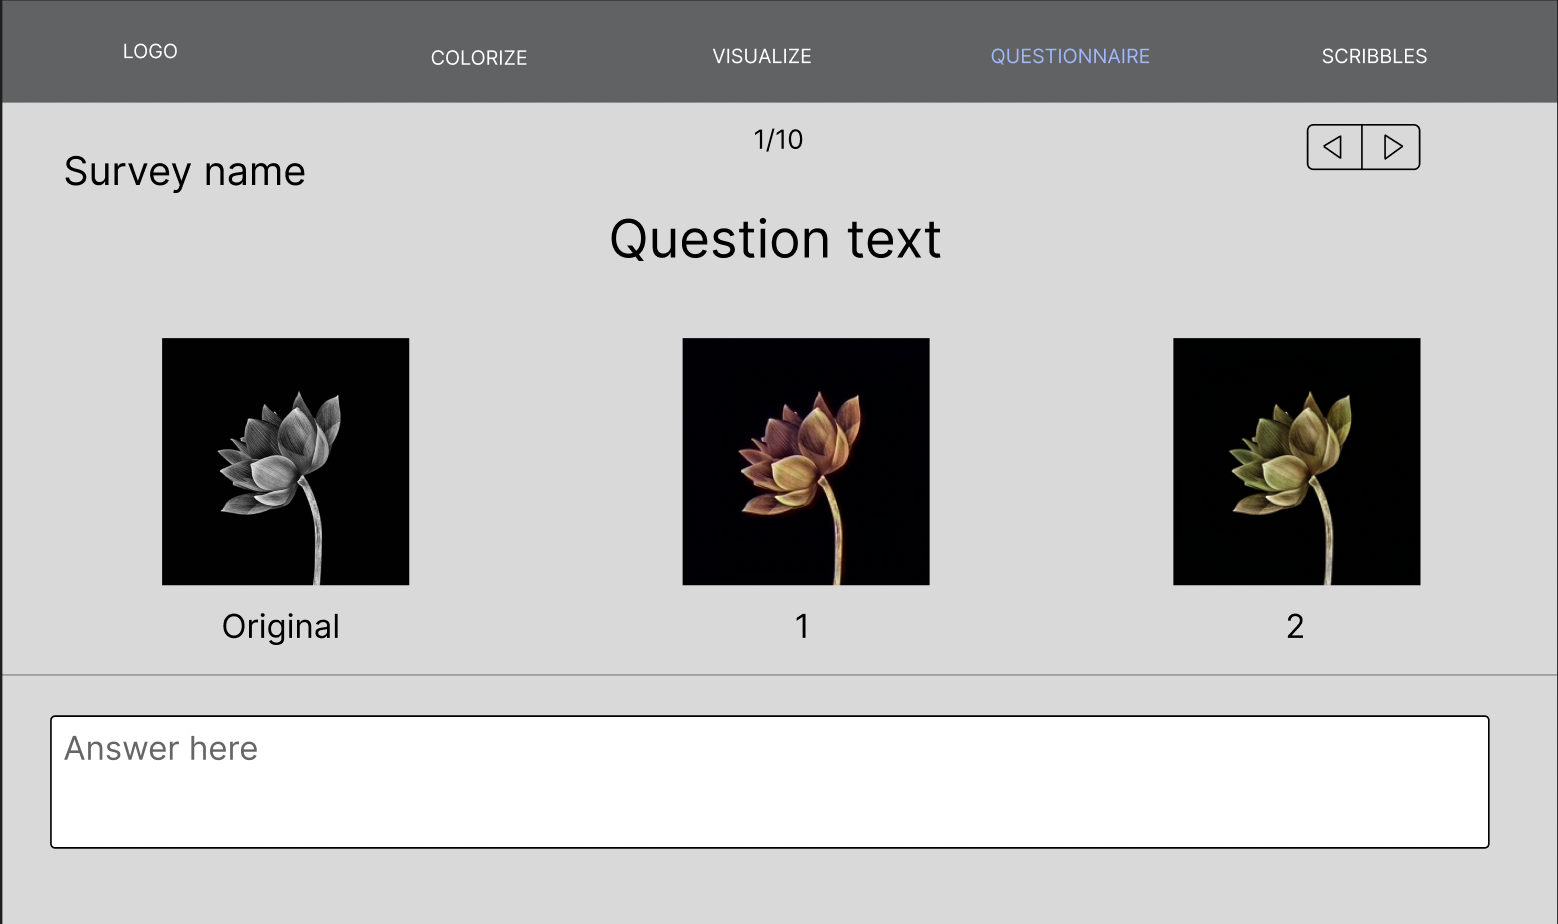
\includegraphics[width=11cm]{questionnaire-repondre.png}
    \caption{Maquette : répondre à un questionnaire}
    \label{fig:questionnaire-repondre}
\end{figure}

Sur cet écran, plusieurs choses sont affichées. D'abord, il y a le nom du questionnaire (\textit{Survey Name}), la question (\textit{Question text}), le numéro de
la question, le nombre de questions au total ainsi que les images concernées. Des flèches en haut à droite permettent de naviguer entre les questions.
Enfin, en bas de l'écran, les champs de réponse sont affichés. Ici, il s'agit d'un champ de texte mais cela dépend du type de la question.

Le dernier aspect des questionnaires (visualiser les réponses) a été modélisé dans la figure \ref{fig:questionnaire-visualiser-reponse}.

\begin{figure}[!ht]
    \centering
    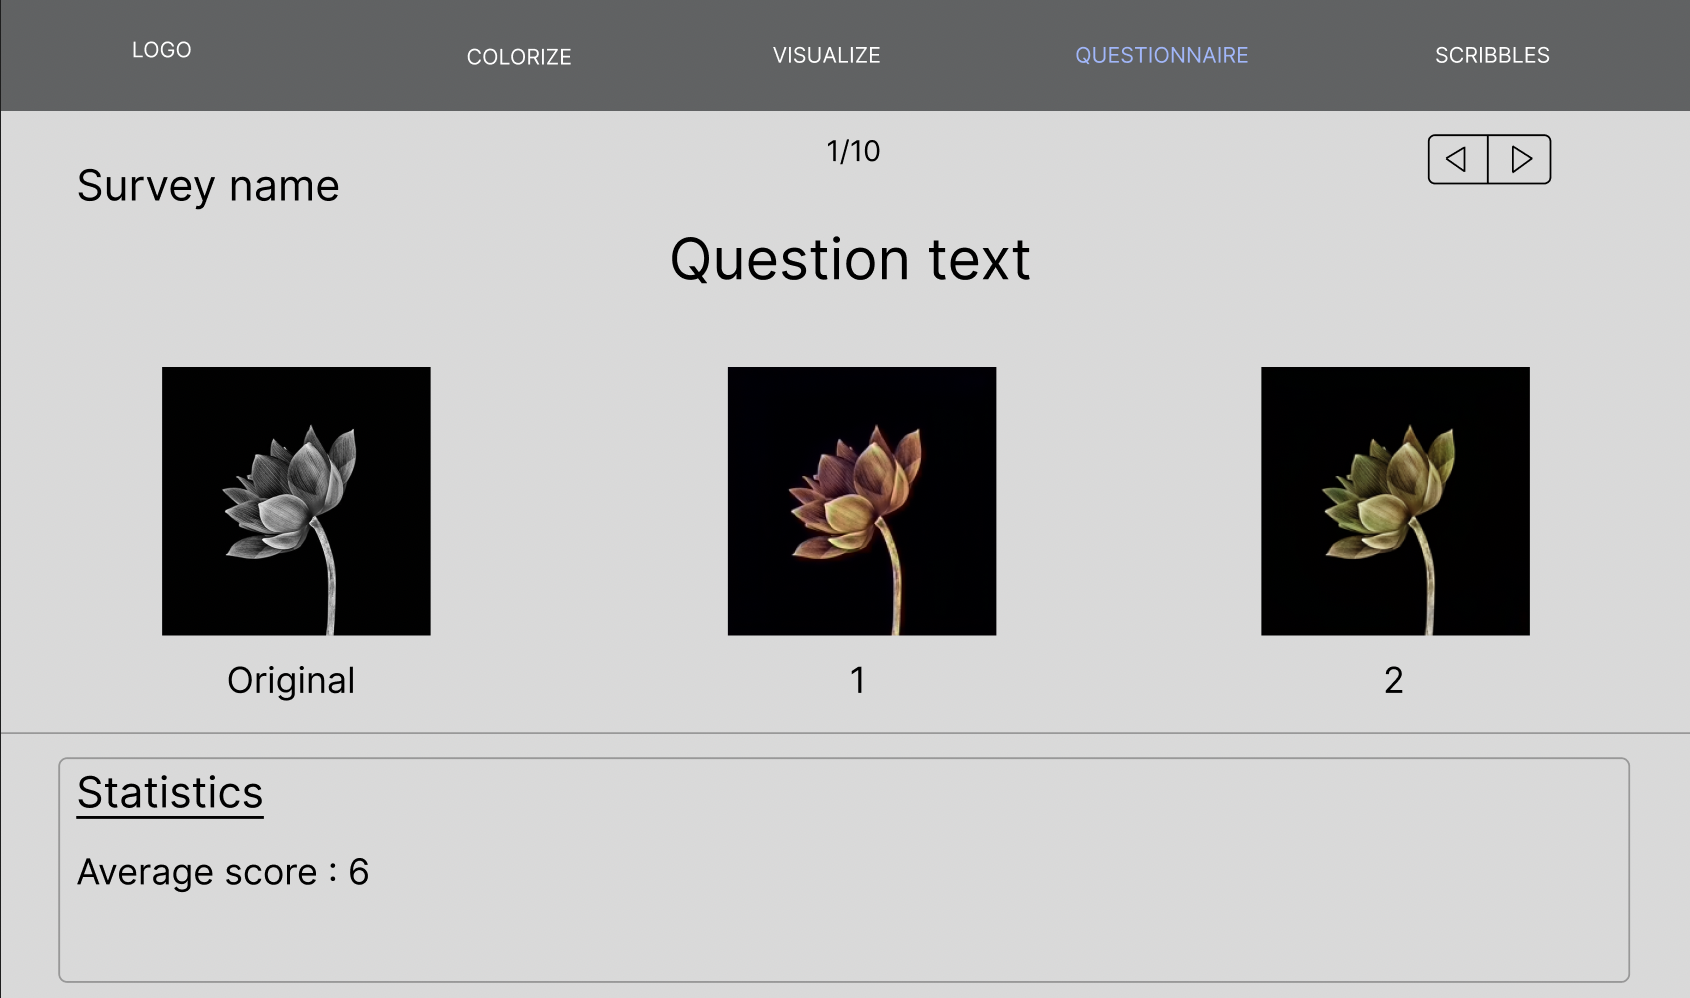
\includegraphics[width=11cm]{questionnaire-visualiser-reponse.png}
    \caption{Maquette : visualiser les réponses à un questionnaire}
    \label{fig:questionnaire-visualiser-reponse}
\end{figure}

Sur cette interface, les mêmes informations sur la question sont affichés que dans l'interface précédente. Cependant,
au lieu d'avoir des champs de réponse, il y a toutes les réponses qui ont été enregistrées pour cette question et éventuellement des statistiques les concernant 
(surtout pour des questions à caractère quantitatif).

\subsection{Implémentation de certaines fonctionnalités} \label{implementation-code}
Au cours de la première phase de ce projet, nous avons réussi à mettre en place un début de solution fonctionnelle qui satisfait certaines exigences du client. Les réalisations effectuées permettent de charger un ensemble 
d'images noir et blanc via une interface web, puis de les coloriser en utilisant un modèle 
d'apprentissage profond (\texttt{ChromaGAN}). Nous avons choisi de commencer par ce modèle car il s'exécute de manière automatique
et ne requiert aucune action de l'utilisateur. Les images colorisées sont ensuite organisées dans des répertoires en suivant une architecture précise qui a été définie en section \ref{sec:archi-detaillee}.

Pour arriver à ce résultat, nous avons commencé tout d’abord par la configuration du serveur \texttt{Flask}, afin de mettre en place l’architecture MVC en créant des fichiers pour les vues, les modèles et les contrôleurs, chacun gérant une partie spécifique de l'application. 
Les vues gèrent les interfaces utilisateur créées en utilisant \texttt{ReactJS} (qui a donc été intégré et configuré pour le projet), les modèles représentent les données de l'application et les contrôleurs 
gèrent les interactions entre les vues et les modèles.

En outre, une fonctionnalité de chargement d'images individuelles ou de dossiers d'images a été ajoutée, permettant aux utilisateurs de les charger pour être traités par l'application en utilisant 
l’interface de la figure \ref{fig:chargement}.

\begin{figure}[!h]
    \centering
    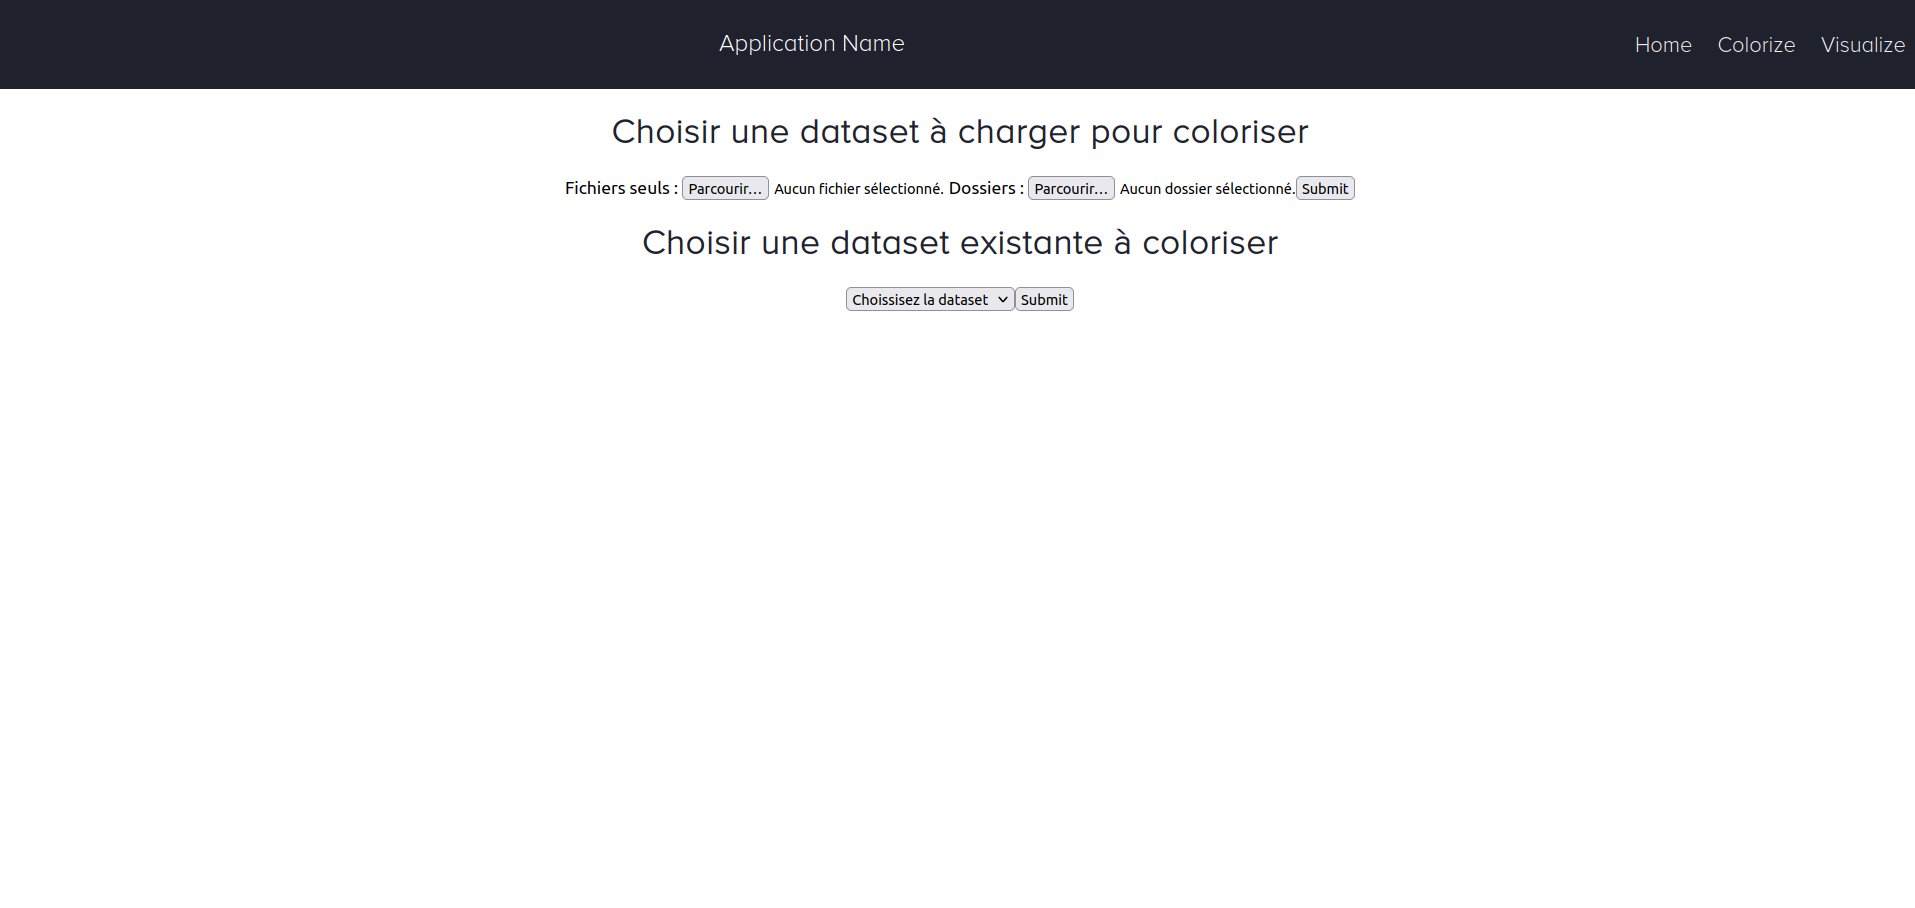
\includegraphics[width=15cm]{img/interface-chargement.png}
    \caption{Interface actuelle de chargement des images}
    \label{fig:chargement}
\end{figure}

Après avoir chargé les images et en cliquant sur le bouton \textit{submit}, une requête \texttt{POST} est envoyée au serveur \texttt{Flask} pour coloriser toutes les images chargées en utilisant le modèle d'apprentissage profond \texttt{ChromaGAN}. Les résultats de 
cette colorisation sont affichés sur l'interface de la figure \ref{fig:visualisation}. L’utilisateur peut également visualiser des colorisation effectuées précédemment à l'aide de l'interface de la figure \ref{fig:choix}.

Pour éviter la duplication des images originales, nous avons ajouté à l'interface de la figure \ref{fig:chargement}, la possibilité d’utiliser un jeu 
de données déjà chargé pour ensuite appliquer le service de colorisation.


\begin{figure}[!h]
    \centering
    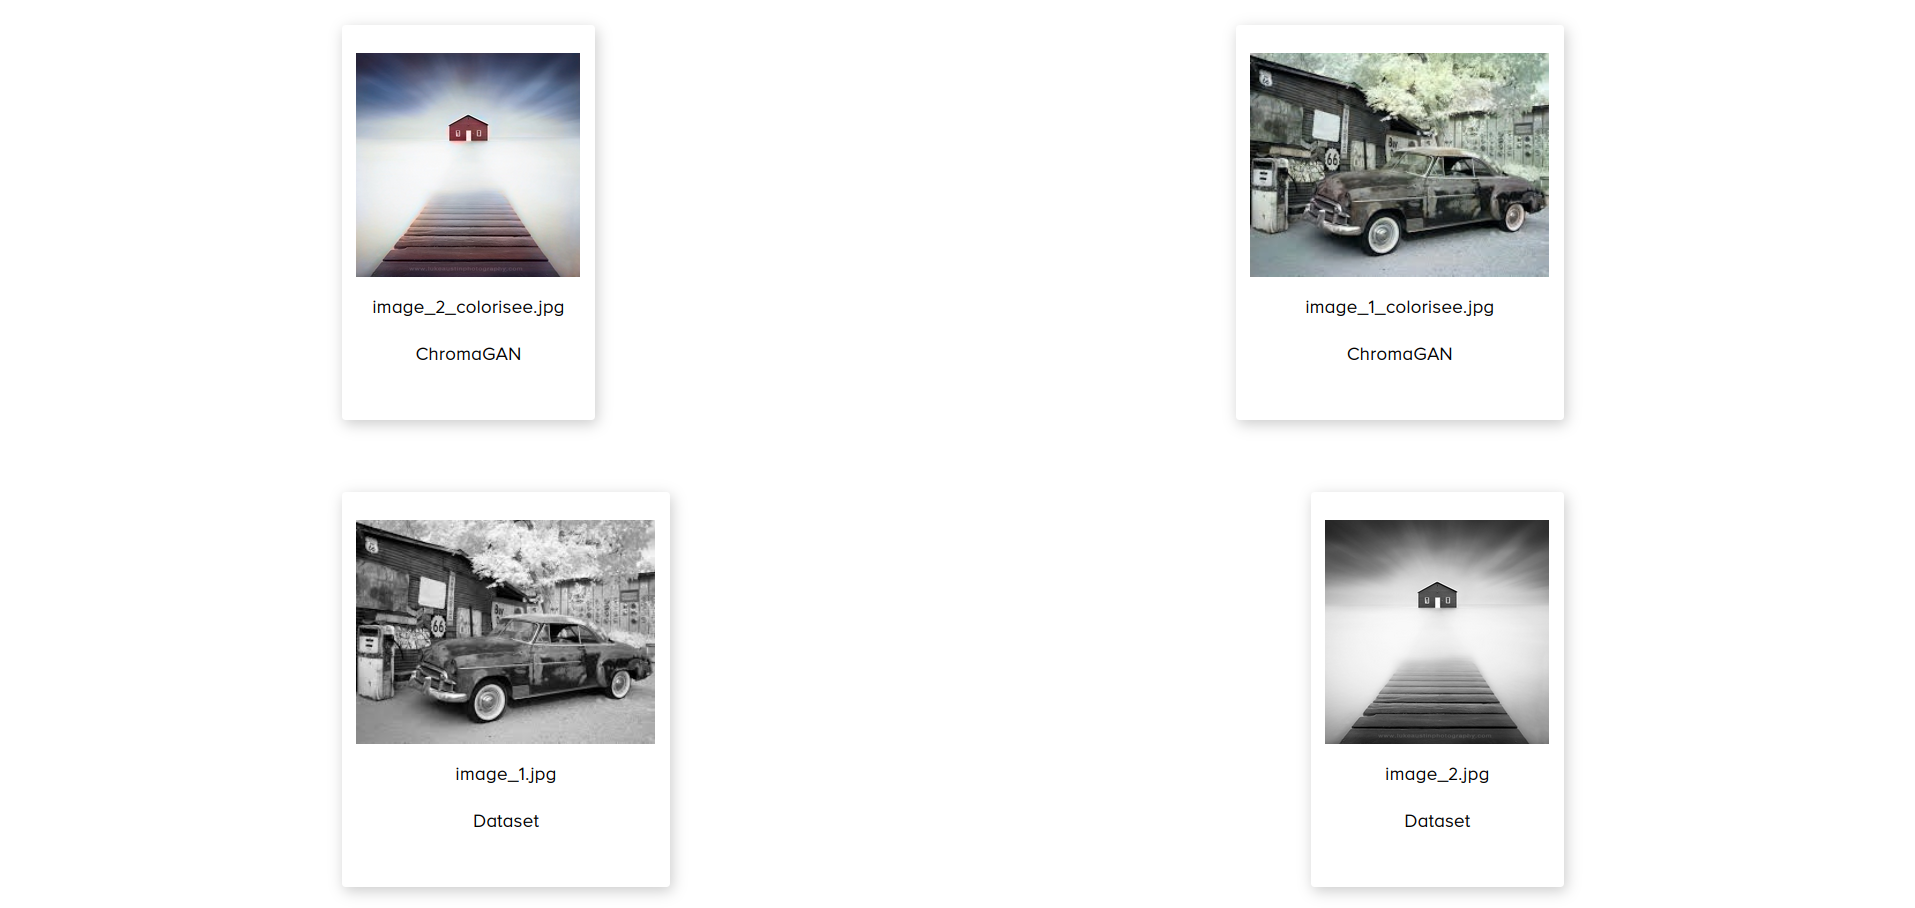
\includegraphics[width=15cm]{img/interface-visualisation.png}
    \caption{Interface actuelle de visualisation des résultats d'une colorisation}
    \label{fig:visualisation}
\end{figure}

\begin{figure}[!h]
    \centering
    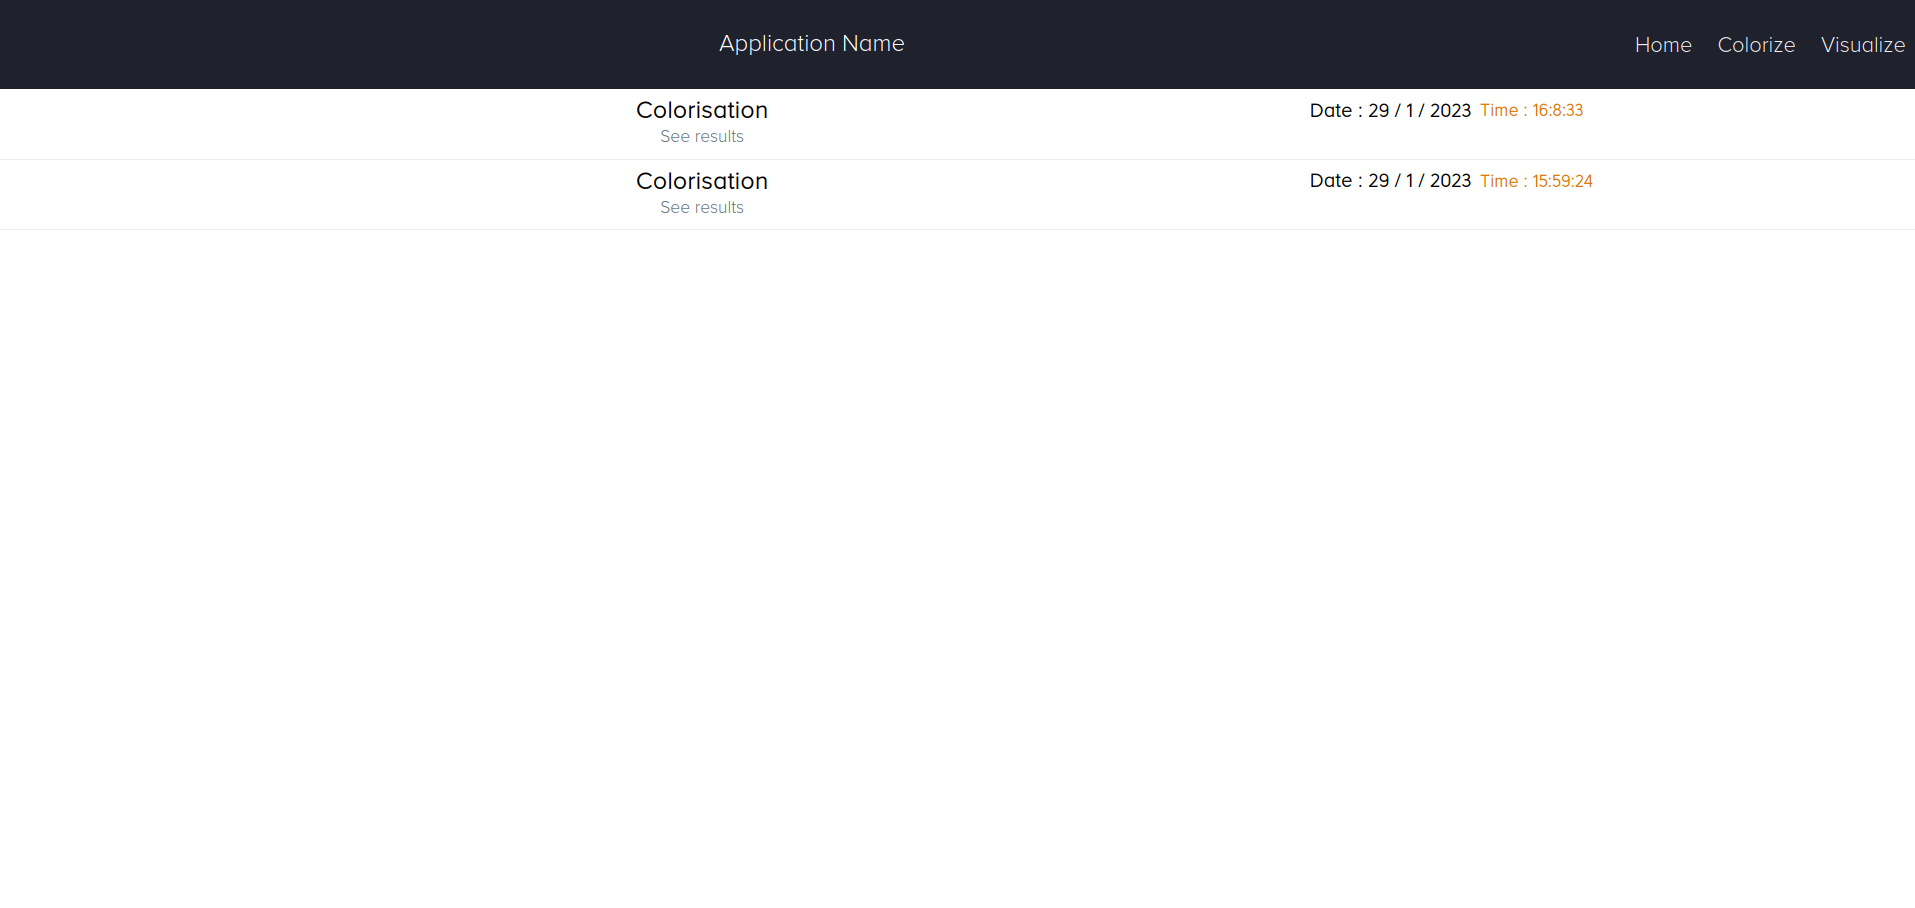
\includegraphics[width=15cm]{img/choix-resultat.png}
    \caption{Interface actuelle listant les colorisations effectuées}
    \label{fig:choix}
\end{figure}

\newpage
\section{Conclusion}

Pour résumer, ce projet a pour objectif de créer une application aidant les chercheurs à utiliser et évaluer des méthodes de colorisation par \emph{deep-learning}.
Afin de mieux comprendre les demandes du client, nous avons fait une analyse fonctionnelle du sujet en explicitant des fonctionnalités sous la forme de \emph{use cases} et \emph{user stories}, les plus exhaustives possible.
Nous les avons ensuite mis à jour régulièrement en fonction des remarques et ajouts du client lors des réunions que nous avons pu avoir avec lui.
Durant ces réunions nous lui avons présenté des maquettes de l'interface du logiciel, selon l'approche \emph{design first}, afin d'avoir une idée claire et compréhensible par tous de ce qui est attendu.
Ainsi nous avons identifié trois axes principaux : la colorisation, la visualisation des résultats et la création de questionnaires d'évaluation.
Chacun de ces axes sera réalisé indépendamment, en utilisant un modèle Client-Serveur avec des technologies choisies en fonction de nos besoins : un serveur, appelé \emph{Back-End}, avec \texttt{Flask} et un client, appelé \emph{Front-End}, avec \texttt{ReactJS}.
Le développement sera organisé en suivant la méthode agile, qui préconise de travailler en courtes itérations appelées \emph{sprints} durant lesquelles un nombre prédéfini d'\emph{user stories} seront réalisées.
Cette façon de faire permet d'avoir un suivi régulier de l'avancement du projet ainsi qu'un retour du client. Nous avons déjà appliqué cette méthode pour commencer à développer les bases du projet ; cela nous a permis de mieux estimer le temps nécessaire et de minimiser les risques d'une mauvaise organisation.
L'application actuelle permet de charger des images, de lancer une colorisation avec un unique modèle non paramétrable et de visualiser les résultats dans une interface très basique.

Ce document rassemble donc ce que nous avons interprété du sujet, les spécifications du logiciel que nous développerons afin de répondre au besoin du client, et la manière dont nous le réaliserons.
Il servira de référence pendant toute la mise en oeuvre, mais le plus important restera la flexibilité et l'adaptation au client si ses attentes et besoins changent au cours du projet. Une évolution de ce cahier des charges sera alors possible.


\pagebreak
\appendix

\appendixpage
\addappheadtotoc

\section{État de l'art}

La colorisation d'une image en noir et blanc est un problème complexe dont les solutions existantes
peuvent encore être perfectionnées.
Ainsi, de nombreuses méthodes différentes existent afin de donner de la couleur à une image.
La plupart des méthodes actuelles sont des méthodes de \textit{deep learning} et utilisent des réseaux neuronaux complexes,
permettant de coloriser correctement différentes parties d'une image. Cependant, ces méthodes diffèrent grandement
dans l'architecture de leurs réseaux neuronaux, leurs techniques d'apprentissages ou encore les moyens qu'elles emploient pour résoudre
certains problème de colorisation connus (comme le \textit{color-bleeding}, autrement dit le débordement de certaines couleurs sur d'autres objets). 
De plus, une fois les images colorisées, il peut être compliqué d'évaluer la qualité de la colorisation effectuée. La perception des couleurs est avant
tout une expérience intrinsèque, propre à chacun, qui dépend donc de l'interprétation individuelle de chaque individu.
Mesurer la qualité d'une colorisation peut donc s'avérer difficile. Certaines métriques existent et comparent l'image colorisée avec l'image d'origine.
Dans les sections suivantes, les différentes méthodes de colorisation qui existent ainsi que les manières de les évaluer seront 
présentées.

\subsection{Les différentes méthodes de colorisation}

Deux types de colorisation peuvent être distingués. On différencie donc les méthodes qui auront besoin 
d'une contribution extérieure (d'un \textit{input}) pour coloriser une image et celles qui peuvent coloriser
une image sans aucun apport additionnel. 

\subsubsection{Méthodes avec participation de l'utilisateur}

Les techniques de colorisation présentées dans cette section ont besoin d'un \textit{input} 
afin de coloriser une image. 

\paragraph{Avec des scribbles}
Les \emph{scribbles} sont des points ou traits de couleurs donnés par l'utilisateur sur l'image en noir et blanc.

Ces traits de couleurs se révèlent très utiles pour coloriser des images de manière plus précise.
Ainsi, ils peuvent par exemple être utiles pour distinguer les objets entre eux et éviter le problème du \textit{color-bleeding} (Kim \emph{et al}., 2021 \cite{color-Bleeding}).
Dans leur article, ils montrent que si l'utilisateur dessine des \textit{scribbles} aux frontières d'objets qui pourraient ne pas
être bien différenciés (qui partagent des niveaux de gris très similaires), la colorisation s'améliore nettement. Leur réseau neuronal a été entraîné à l'aide de ces traits.
Pour éviter de demander à des utilisateurs de générer des \textit{scribbles} pour un grand nombre d'images, ils ont créé un algorithme permettant de générer 
des pseudo-scribbles pour entraîner le réseau neuronal. %% à préciser plus ?

Les traits colorés peuvent également être utilisés pour indiquer au réseau de neurone la couleur désirée pour une zone
précise de la photo. Cette couleur est propagée à tous les pixels ayant la même intensité de gris que les points marqués.
C'est ce qu'ont fait Levin \emph{et al}. \cite{10.1145/1015706.1015780} en démontrant que seulement quelques traits de couleur 
étaient suffisant pour produire une colorisation de qualité. Ce principe peut être étendu. Sangkloy \emph{et al}. \cite{journals/corr/SangkloyLFYH16} ont développé 
un algorithme permettant d'obtenir une image coloré à partir d'une esquisse et de \textit{scribbles} colorés. Leur algorithme
peut être étendu à la colorisation d'images en niveaux de gris car leur réseau neuronal est capable de distinguer les différents éléments sémantiques
(les différents objets) d'une image.

Des algorithmes sont également développés pour prendre à la fois des entrées dites 'locales' et des entrées dites 'globales'.
Les entrées locales sont définies comme des points de couleur positionnées localement sur l'image tandis que les entrées globales sont 
des informations plus générales comme un histogramme de couleurs.
Ainsi, Zhang \emph{et al}. \cite{ZhangZIGLYE17} ont développé un réseau neuronal qui peut prendre soit des informations locales comme des points de couleurs sur l'image,
soit des informations globales.
Xiao \emph{et al}. \cite{abs-1801-09083} ont quant à eux développé une architecture qui offre le choix à l'utilisateur : soit il ne donne pas d'entrée additionnelle pour coloriser
son image, soit il donne des entrées locales, soit il donne des entrée globales ou soit il donne simultanément ces deux types d'entrées.


%\begin{itemize}
    % done \item \href{https://arxiv.org/pdf/2107.01619.pdf}{Deep Edge-Aware Interactive Colorization against Color-Bleeding Effects} 
    % done \item \href{https://arxiv.org/pdf/1705.02999.pdf}{Real-Time User-Guided Image Colorization with Learned Deep Priors}
    % done \item \href{https://webee.technion.ac.il/people/anat.levin/papers/colorization-siggraph04.pdf}{Colorization using Optimization} %% traits de couleurs directement sur l'image
    % done \item \href{https://arxiv.org/pdf/1801.09083.pdf}{Interactive Deep Colorization With Simultaneous Global and Local Inputs} %%soit rien , soit les deux , soit l'un , soit l'autre : à la fois des local inputs (points de couleur)
    % done \item \href{https://arxiv.org/abs/1612.00835}{Scribbler: Controlling Deep Image Synthesis with Sketch and Color}
%\end{itemize}

\paragraph{Avec des références}
Une référence est une image dont on utilise les couleurs pour coloriser une image en niveaux de gris.

Ces méthodes de colorisation visent à diminuer les efforts d'un utilisateur qui souhaite coloriser une image.
En effet, lorsqu'un utilisateur souhaite coloriser une image en utilisant des \textit{scribbles}, dessiner les traits
en choisissant les bonnes couleurs peut parfois s'avérer long.

Welsh \emph{et al}. \cite{10.1145/566654.566576} ont élaboré un algorithme permettant de coloriser une image avec des actions minimales de l'utilisateur.
Leur méthode permet à l'utilisateur de choisir certaines régions d'une image de référence dont il souhaite déporter la couleur et 
% à compléter

Certaines méthodes de colorisation par référence ont également été développées afin d'utiliser plusieurs images de références.
Ainsi, Liu \emph{et al}. \cite{10.1145/1409060.1409105} ont développé un algorithme permettant d'obtenir des images de références grâce à des 
recherches internet. Les images de références sont donc diverses car elles représentent une scène similaire sous un angle différent ou avec une 
luminosité différente. Les couleurs de ces images sont transférées à l'image souhaitée.

De plus, Irony \emph{et al.} \cite{10.5555/2383654.2383683} ont créé un algorithme de colorisation prenant en paramètre une image de référence. Leur 
méthode repose sur une segmentation des images. L'image de référence est séparée en plusieurs sections, tout comme 
l'image en noir et blanc qu'on souhaite coloriser. La couleur de chaque pixel de l'image à coloriser est déterminée
en l'associant à une des sections de l'image de référence. Pour faire fonctionner cette méthode,
il suffit donc que l'utilisateur ne fournisse qu'une seule image de référence.

D'autres méthodes de colorisation se basent sur des superpixels comme celle de Gupta \emph{et al.} \cite{10.1145/2393347.2393402}. Les superpixels sont des groupes
de pixels d'une image et permettent de segmenter l'image en plusieurs parties. Leur algorithme consiste à associer des superpixels 
de l'image de référence et de l'image d'origine en noir et blanc pour leur associer la bonne couleur.
Cette technique permet d'accélérer le processus de colorisation.

Enfin, la colorisation par référence peut aussi parfois s'effectuer avec des images de références qui ne sont pas sémantiquement
reliées à l'image qu'on souhaite coloriser. Ainsi, c'est le cas d'une méthode de He \emph{et al.} \cite{journals/corr/abs-1807-06587} qui permet de coloriser une image à partir
de plusieurs références. Leur algorithme permet également de suggérer des images de référence à l'utilisateur automatiquement.




% \begin{itemize}
%     % done \item \href{https://www3.cs.stonybrook.edu/~mueller/papers/colorize-final.pdf}{Transferring Color to Greyscale Images}
%     % done \item \href{http://www.cse.cuhk.edu.hk/~ttwong/papers/incolor/paper/incolor.pdf}{Intrisic Colorization}
%     % done \item \href{https://www.cs.tau.ac.il/~dcor/online_papers/papers/colorization05.pdf}{Colorization by Example}
%     % done \item \href{https://www.researchgate.net/publication/262353941_Image_colorization_using_similar_images}{Image Colorization using similar images}
%     % done \item \href{https://arxiv.org/pdf/1807.06587.pdf}{Deep Exemplar-based Colorization}
% \end{itemize}

\paragraph{Avec du texte}
Il est possible d'utiliser des méthodes de traitement du langage naturel pour aider à la colorisation.
Ces méthodes, moins courantes, se basent sur une description textuelle d'une image pour la coloriser. 

Manjunatha \emph{et al}. \cite{journals/corr/abs-1804-06026} ont ainsi développé deux algorithmes permettant de coloriser une image à partir d'une phrase descriptive comme "de l'herbe verte et un ciel gris".
Leurs deux méthodes diffèrent dans leurs nombre de paramètres mais produisent des résultats de qualité équivalente.

Cho \emph{et al}. \cite{journals/corr/abs-1804-04128} ont créé une méthode de colorisation basée sur le texte différente de celle mentionnée précédemment.
Leur méthode est composée de deux parties : une partie d'analyse du texte descriptif permettant de générer une palette de couleur et une partie de colorisation
de l'image à partir de la palette de couleur générée précédemment. Les descriptions données à l'algorithme correspondent plus à des concepts (comme "ensoleillé")
qu'à des descriptions précises de l'image.


% \begin{itemize}
%     % done \item \href{https://arxiv.org/pdf/1804.06026.pdf}{Learning to Color from Language}
%     % done \item \href{https://arxiv.org/pdf/1804.04128.pdf}{Coloring with words: Guiding image colorization through text-based palette generation}
% \end{itemize}

\subsubsection{Méthodes automatiques}

\paragraph{Méthodes simples}
Faire appel à un utilisateur pour aider à la colorisation de chaque image est coûteux en temps.
L'utilisation de réseaux de neurones convolutifs (CNN) entraînés sur des larges bases de données d'images est proposée pour la première fois par Cheng \emph{et al.} \cite{journals/corr/ChengYS16} en 2016.
Plusieurs réseaux sont aussi combinés en un ensemble par Cheng \emph{et al.} \cite{8011494} pour mieux représenter les différents styles de couleurs dans une image.

Cependant ces méthodes sont biaisées par les données sur lesquelles elles sont entraînées, et souffrent d'un manque de couleur vives et réalistes.
Afin de pallier à ce problème Zhang \emph{et al.} \cite{journals/corr/ZhangIE16} proposent d'étudier la colorisation comme une classification et utiliser des méthodes de ré-équilibrage de classes sur les couleurs.

Des applications concrètes de ces modèles se révèlent efficaces, comme par exemple pour l'imagerie radar par Song \emph{et al.} \cite{journals/corr/SongXJ17}.


% \begin{itemize}
    % \item \href{https://arxiv.org/pdf/1603.08511.pdf}{Colorful Image Colorization}
    % \item \href{https://sci-hub.wf/10.1109/TIP.2017.2740620}{Colorization Using Neural Network Ensemble}
    % \item \href{https://arxiv.org/pdf/1707.07225v1.pdf}{SAR Image Colorization: Converting Single-Polarization to Fully Polarimetric Using Deep Neural Networks}
% \end{itemize}

\paragraph{Méthodes diverses}
En plus des réseaux de convolutions, diverses architectures de réseaux de neurones ont été proposées pour faire de la colorisation.
Cao \emph{et al.} \cite{journals/corr/CaoZZY17} utilisent des réseaux adversariaux génératifs (GAN) pour entraîner un générateur à cette tâche. Ces types de réseaux sont habituellement utilisés pour générer des images à partir de simple bruit.
Plus tard Vitoria \emph{et al.} \cite{ChromaGAN} reprennent cette idée et l'améliorent en prenant en compte la sémantique de l'image.

Dans la même idée, Deshpande \emph{et al.} \cite{journals/corr/DeshpandeLYF16} appliquent un auto-encodeur variationnel (VAE) au problème de la colorisation et obtiennent des résultats qui surpassent les GAN.

Un troisième modèle utilisé en général pour de la génération et de la classification, le réseau à capsules, est adapté à la colorisation par Özbulak \textit{et al.} \cite{CapsNet}. Celui-ci est relativement simple mais les résultats obtenus semblent prometteurs.

D'autres méthodes font passer les informations par plusieurs chemins dans le réseau pour apprendre.
Ainsi, Iizuka \textit{et al.} \cite{10.1145/2897824.2925974} ont développé une méthode complètement automatique (sans apport d'un utilisateur) qui permet de coloriser des images de n'importe quelle résolution.
Leur modèle comporte plusieurs couches dont une qui permet de fusionner les informations calculées sur des petites portions de l'image avec des informations plus globale sur l'image.

% \begin{itemize}
    % done \item \href{https://sci-hub.wf/10.1145/2897824.2925974}{Let there be Color!: Joint End-to-end Learning of Global and Local Image Priors
    % for Automatic Image Colorization with Simultaneous Classification}
    % \item \href{https://arxiv.org/pdf/1908.08307.pdf}{Image Colorization By Capsule Networks}
% \end{itemize}

\subsection{Évaluer les résultats produits par ces méthodes}

\subsubsection{Métriques quantitatives}

De nombreuses métriques quantitatives existent pour calculer la ressemblance entre deux images. Ces métriques sont donc importantes pour évaluer
la qualité de colorisation d'une image par rapport à l'image d'origine (\textit{groundtruth}).
L'enjeu de ces méthodes est de faire une évaluation qui serait similaire à celle d'un humain.
Quelques métriques sont présentées ici. Elles utilisent toutes des aspects différents des images pour faire leur calculs
et il peut être intéressant de les combiner pour avoir une vision globale de la similarité entre deux images.

\paragraph{Peak Signal to Noise Ratio (PSNR)}
C'est une mesure utilisée à l'origine pour mesurer la qualité de compression d'une image.
Elle est calculée pixel à pixel et ne tient donc pas compte de la sémantique spatiale de l'image.

\paragraph{Structural Similarity (SSIM)}
Cette métrique tente de s'approcher de la perception humaine en évaluant la différence de structure (les différents éléments) entre les images plutôt que la différence pixel à pixel.
Elle a été introduite par Wang \textit{et al.} \cite{1284395} en 2004 comme une métriques complémentaires aux autres métriques plus traditionnelles.

\paragraph{Learned Perceptual Image Patch Similarity (LPIPS)}
Cette métrique a été créé par Zhang \textit{et al.} \cite{journals/corr/abs-1801-03924}  pour palier au défauts de certaines métriques qui n'évaluent pas bien la ressemblance entre 2 images sur certains aspects.
Dans leur article, ils remarquent que les réseaux de neurones apprennent naturellement à créer des images qui correspondent mieux à la perception humaine.
Ils proposent alors d'entraîner un réseau de neurones comme métrique sur un jeu de données de jugements humains.
Ainsi, la métrique LPIPS permet de faire des conclusions équivalentes à celles de la perception humaine
quant à l'évalutation de la similarité entre deux images.

\subsubsection{Perception humaine}

L'objectif de la colorisation d'image est soit d'avoir des couleurs réalistes, soit des couleurs agréables à regarder. 
Dans tous les cas, la perception finale sera faite par l'oeil humain. 
Les métriques présentées précédemment, notamment LPIPS, tentent précisément de se rapprocher de l'évaluation d'un humain. 
Celui-ci prendra cependant mieux en compte la sémantique, les formes et le sens de l'image pour en déduire les couleurs.
Il est donc toujours utile et souvent nécessaire de passer par un jugement humain lors de l'évaluation de méthodes de colorisation.

\section{Maquettes}\label{sec:annexe-maquette}
\begin{figure}[htp]
    \centering
    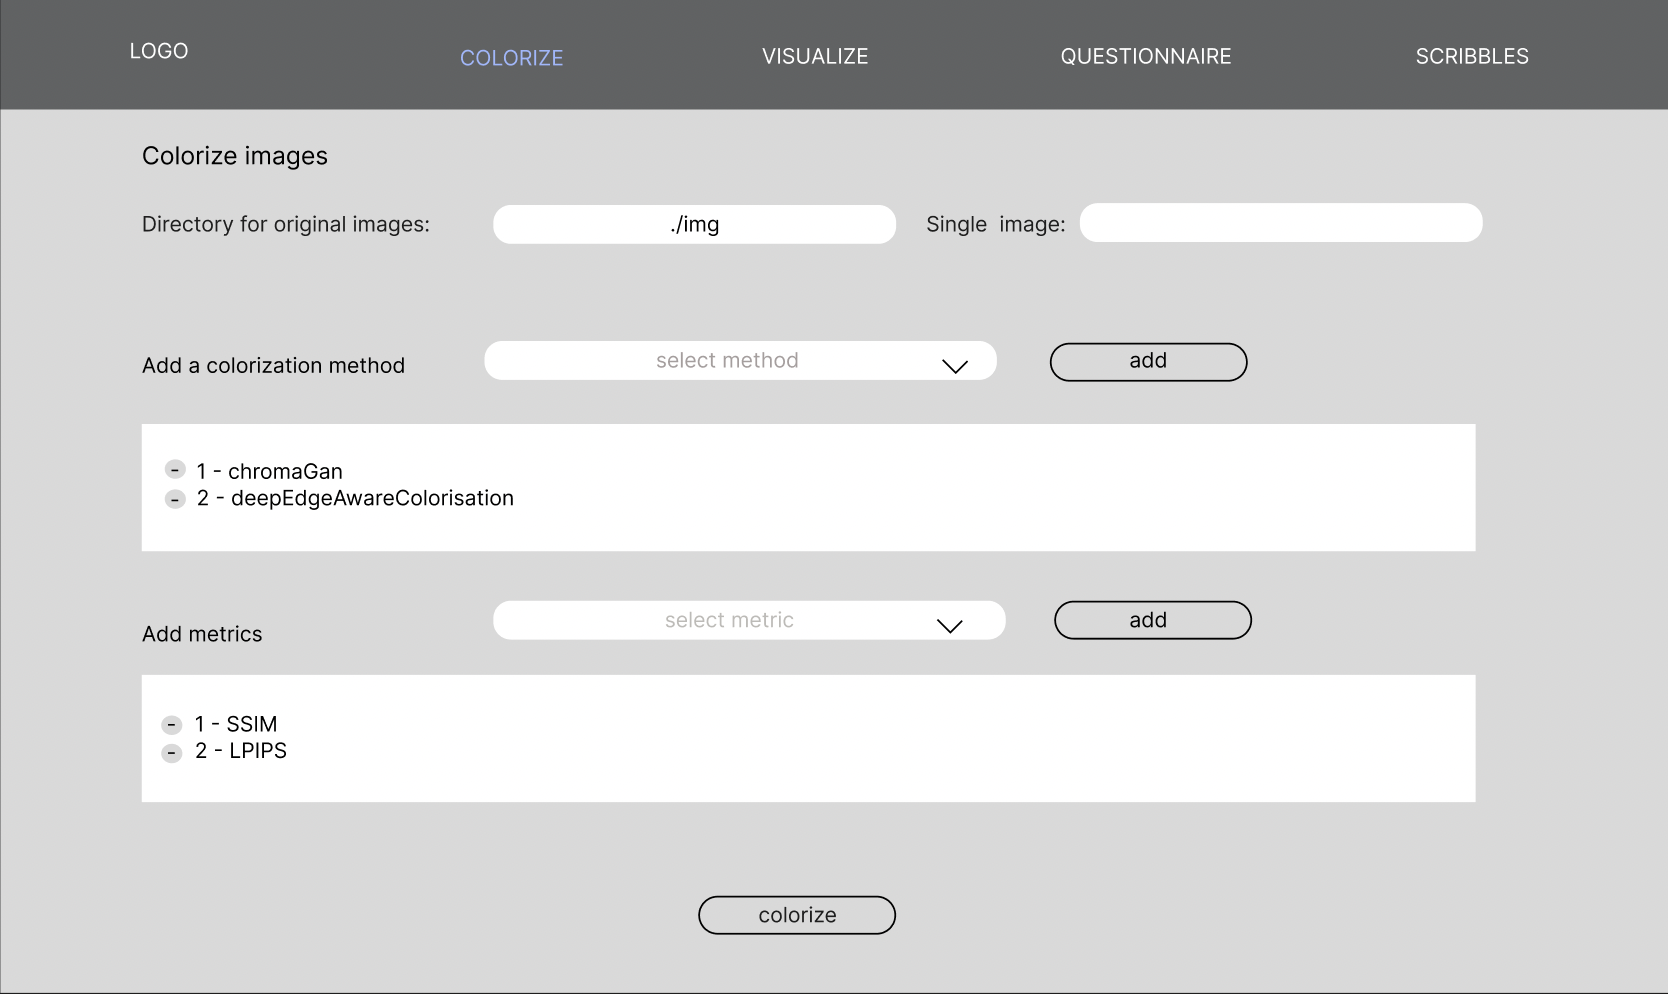
\includegraphics[width=11cm]{coloriser-parametrage1.png}
    \caption{Maquette : paramétrer la colorisation}
    \label{fig:maquette-coloriser-parametrage1}
\end{figure}

\begin{figure}[htp]
    \centering
    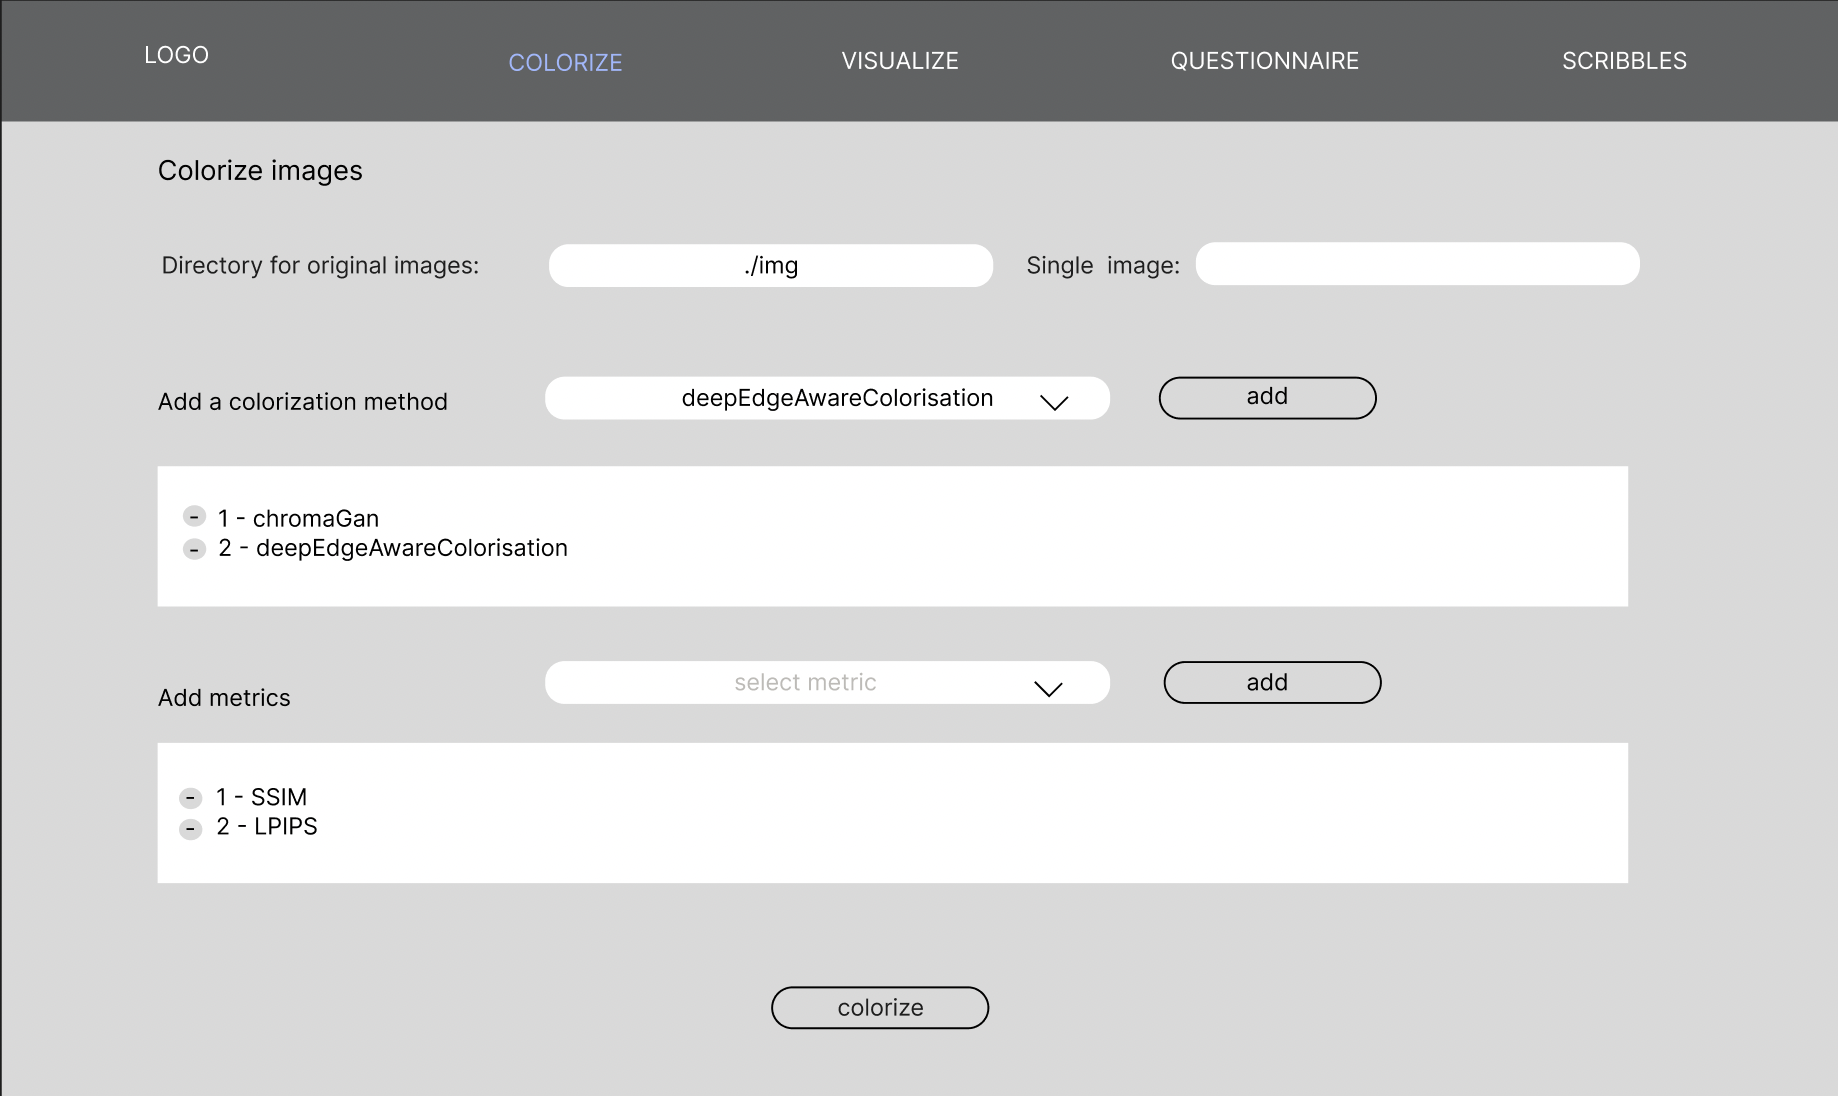
\includegraphics[width=11cm]{coloriser-parametrage2.png}
    \caption{Maquette : paramétrer la colorisation (bis)}
    \label{fig:maquette-coloriser-parametrage2}
\end{figure}

\begin{figure}[htp]
    \centering
    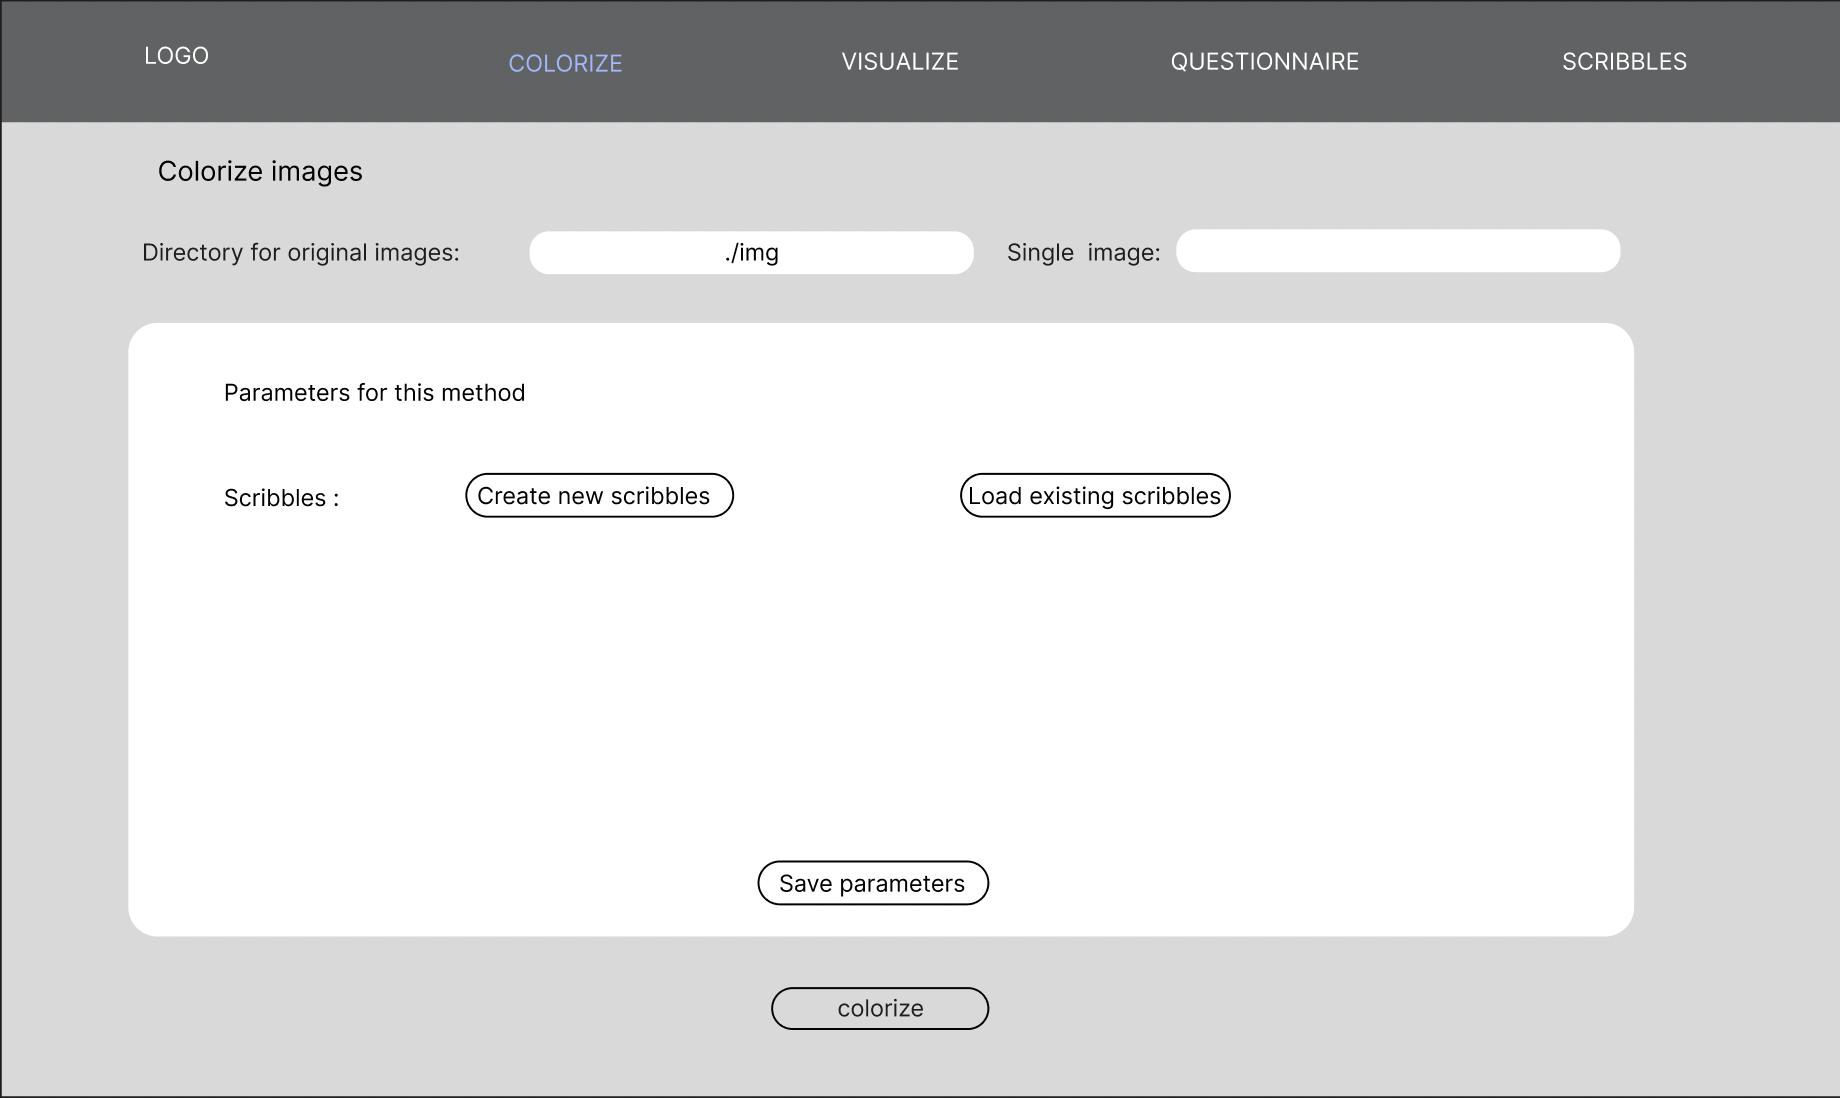
\includegraphics[width=11cm]{coloriser-parametrage3.png}
    \caption{Maquette : paramétrer la colorisation (ter)}
    \label{fig:maquette-coloriser-parametrage3}
\end{figure}


\begin{figure}[htp]
    \centering
    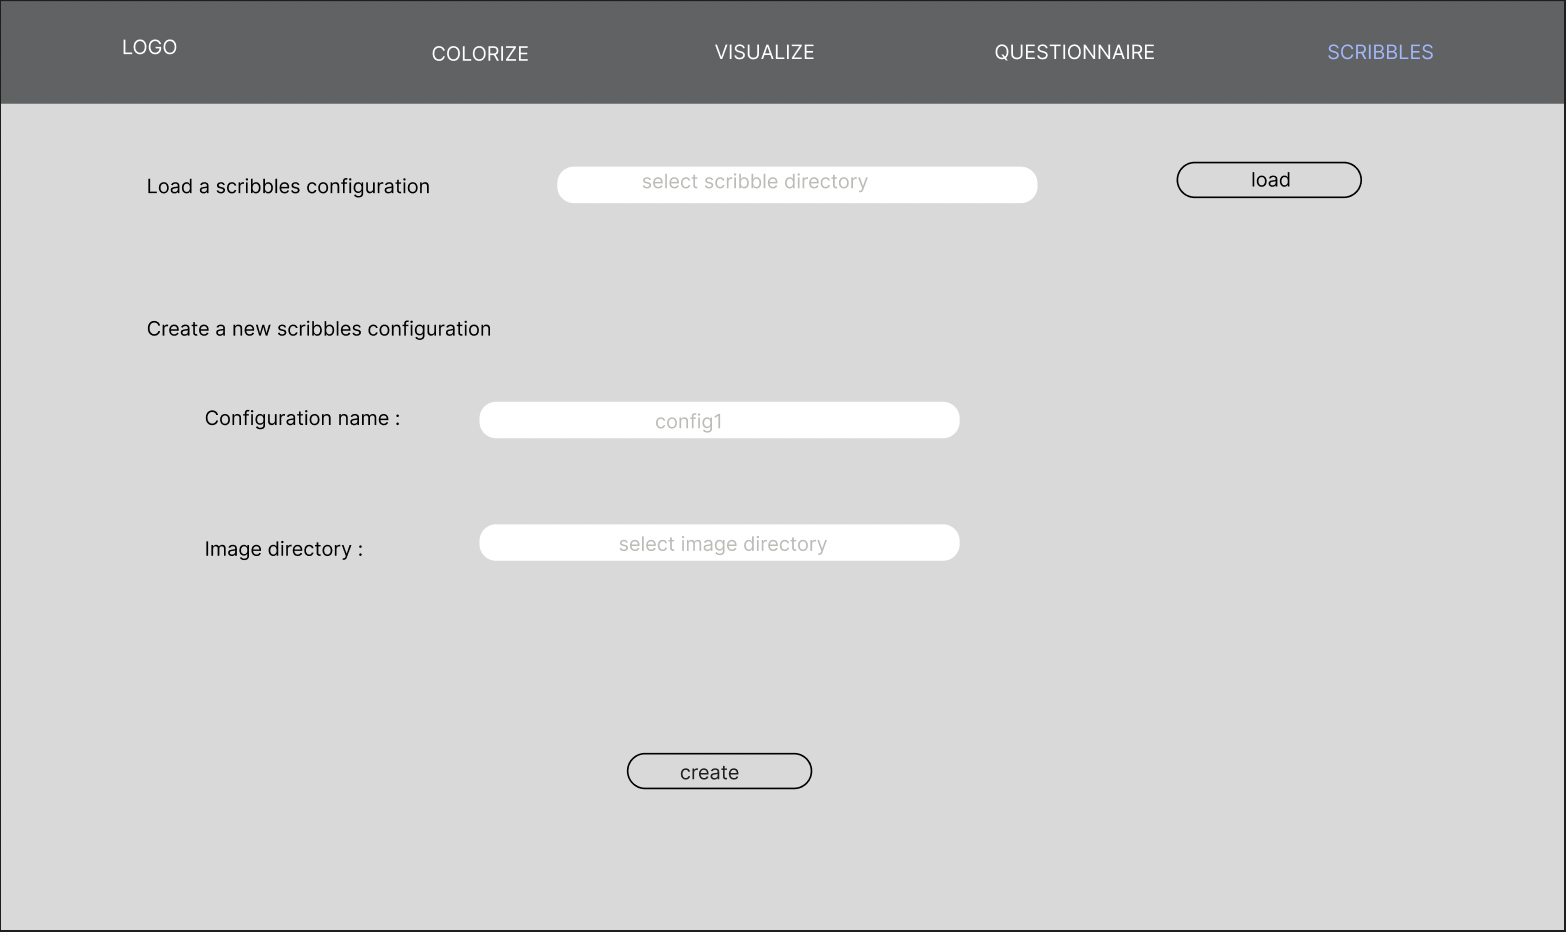
\includegraphics[width=11cm]{coloriser-scribbles-configuration.png}
    \caption{Maquette : configuration des scribbles}
    \label{fig:maquette-coloriser-scribbles-configuration}
\end{figure}   

\begin{figure}[htp]
    \centering
    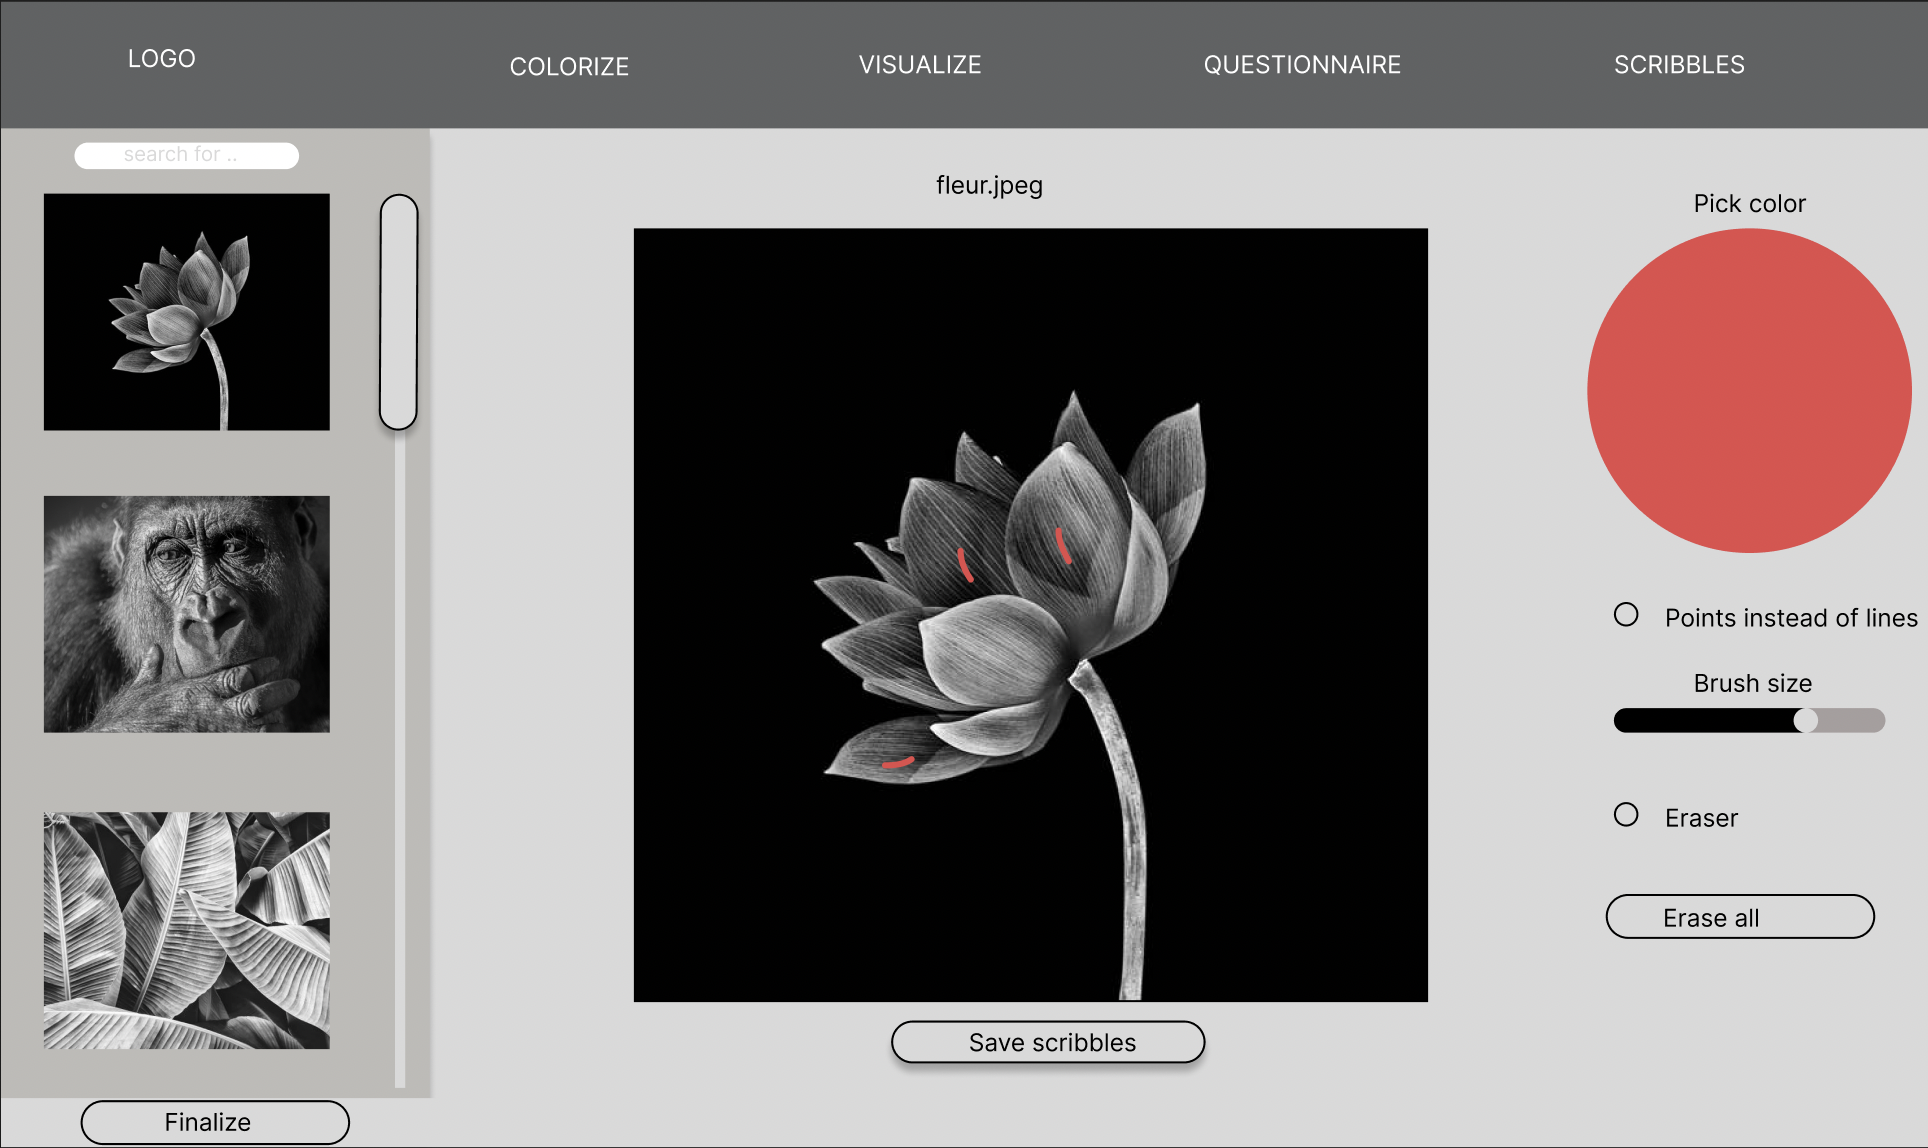
\includegraphics[width=11cm]{coloriser-scribbles.png}
    \caption{Maquette :  créer des scribbles}
    \label{fig:maquette-coloriser-scribbles}
\end{figure} 

\begin{figure}[htp]
    \centering
    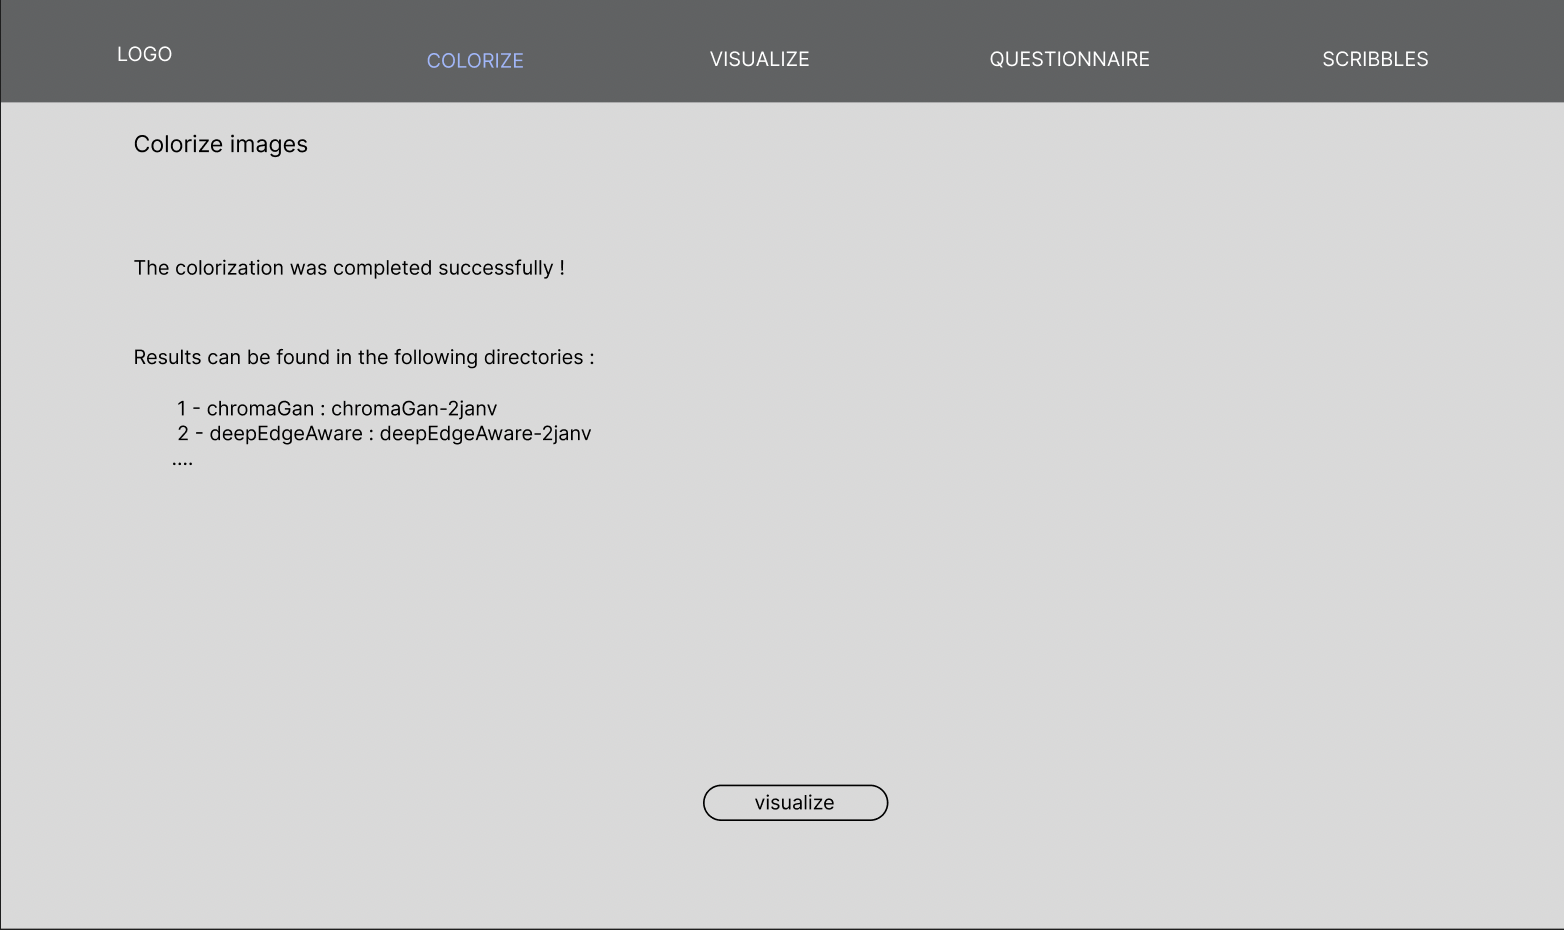
\includegraphics[width=11cm]{coloriser-succes.png}
    \caption{Maquette : une fois la colorisation réussie}
    \label{fig:maquette-coloriser-succes}
\end{figure}

\begin{figure}[htp]
    \centering
    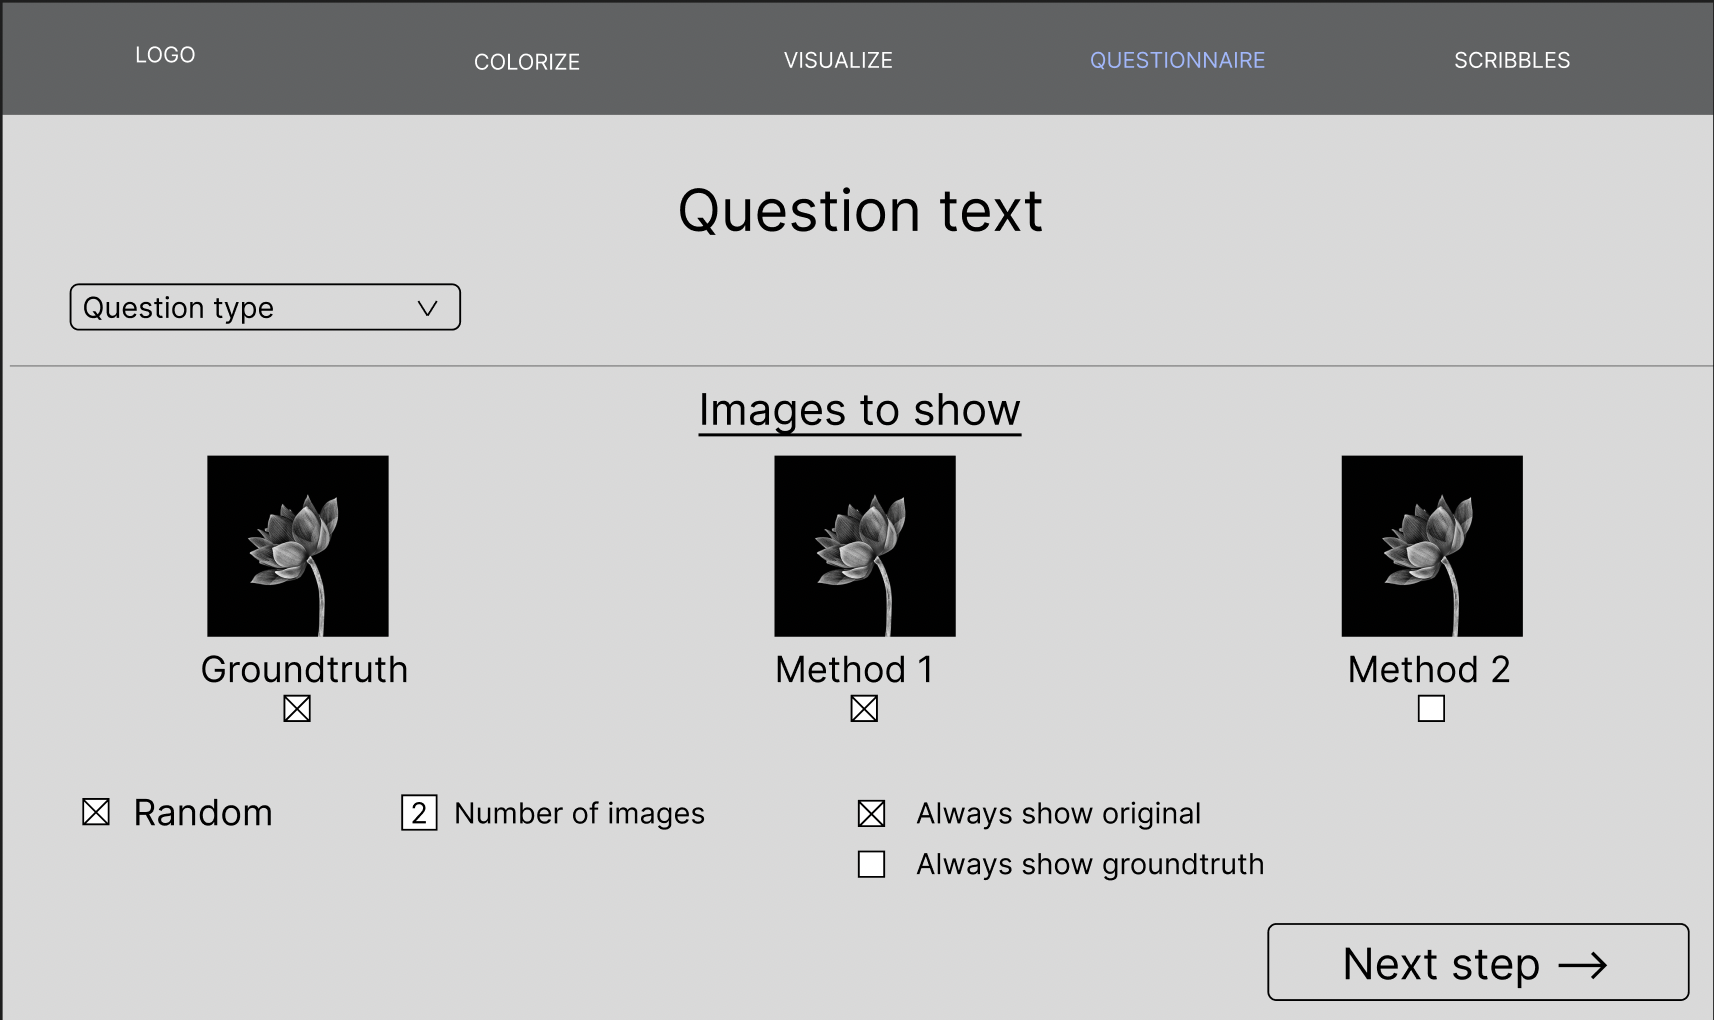
\includegraphics[width=11cm]{questionnaire-creation-question1.png}
    \caption{Maquette : créer une question}
    \label{fig:maquette-questionnaire-creation-question1}
\end{figure}

\begin{figure}[htp]
    \centering
    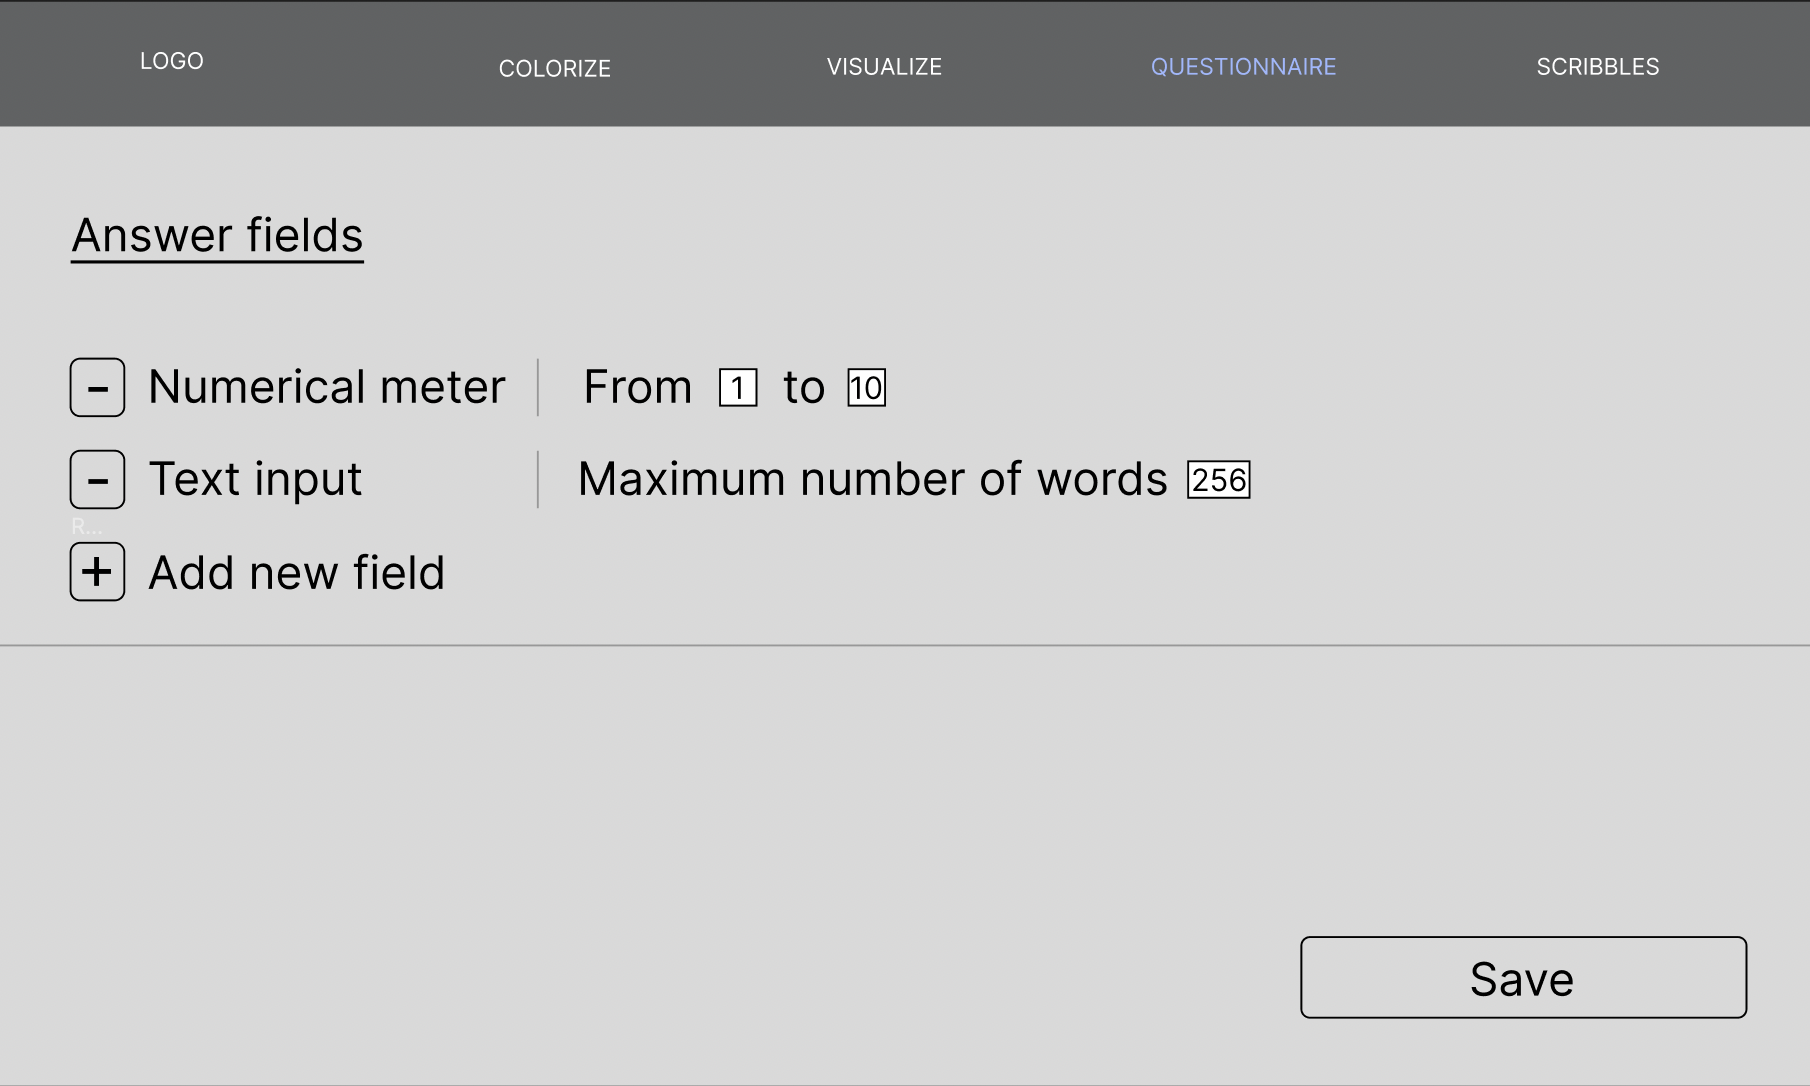
\includegraphics[width=11cm]{questionnaire-creation-question2.png}
    \caption{Maquette : créer une question (bis)}
    \label{fig:maquette-questionnaire-creation-question2}
\end{figure}

\begin{figure}[htp]
    \centering
    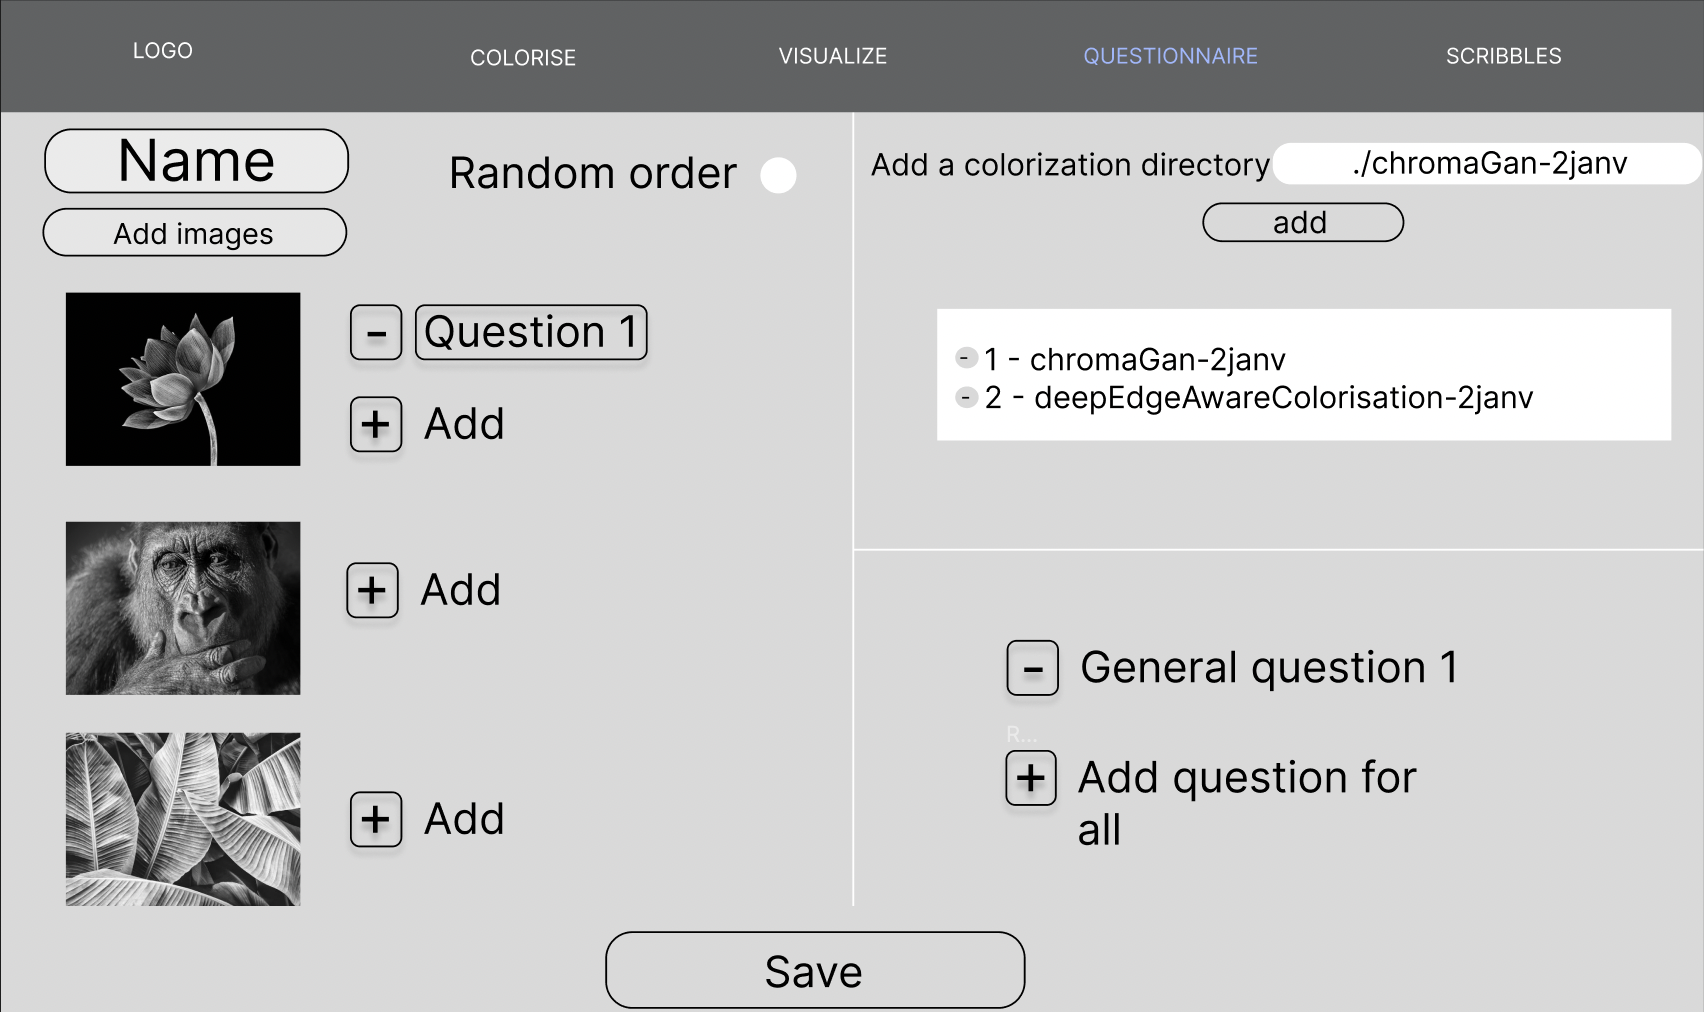
\includegraphics[width=11cm]{questionnaire-creation.png}
    \caption{Maquette : créer un questionnaire}
    \label{fig:maquette-questionnaire-creation}
\end{figure}

\begin{figure}[htp]
    \centering
    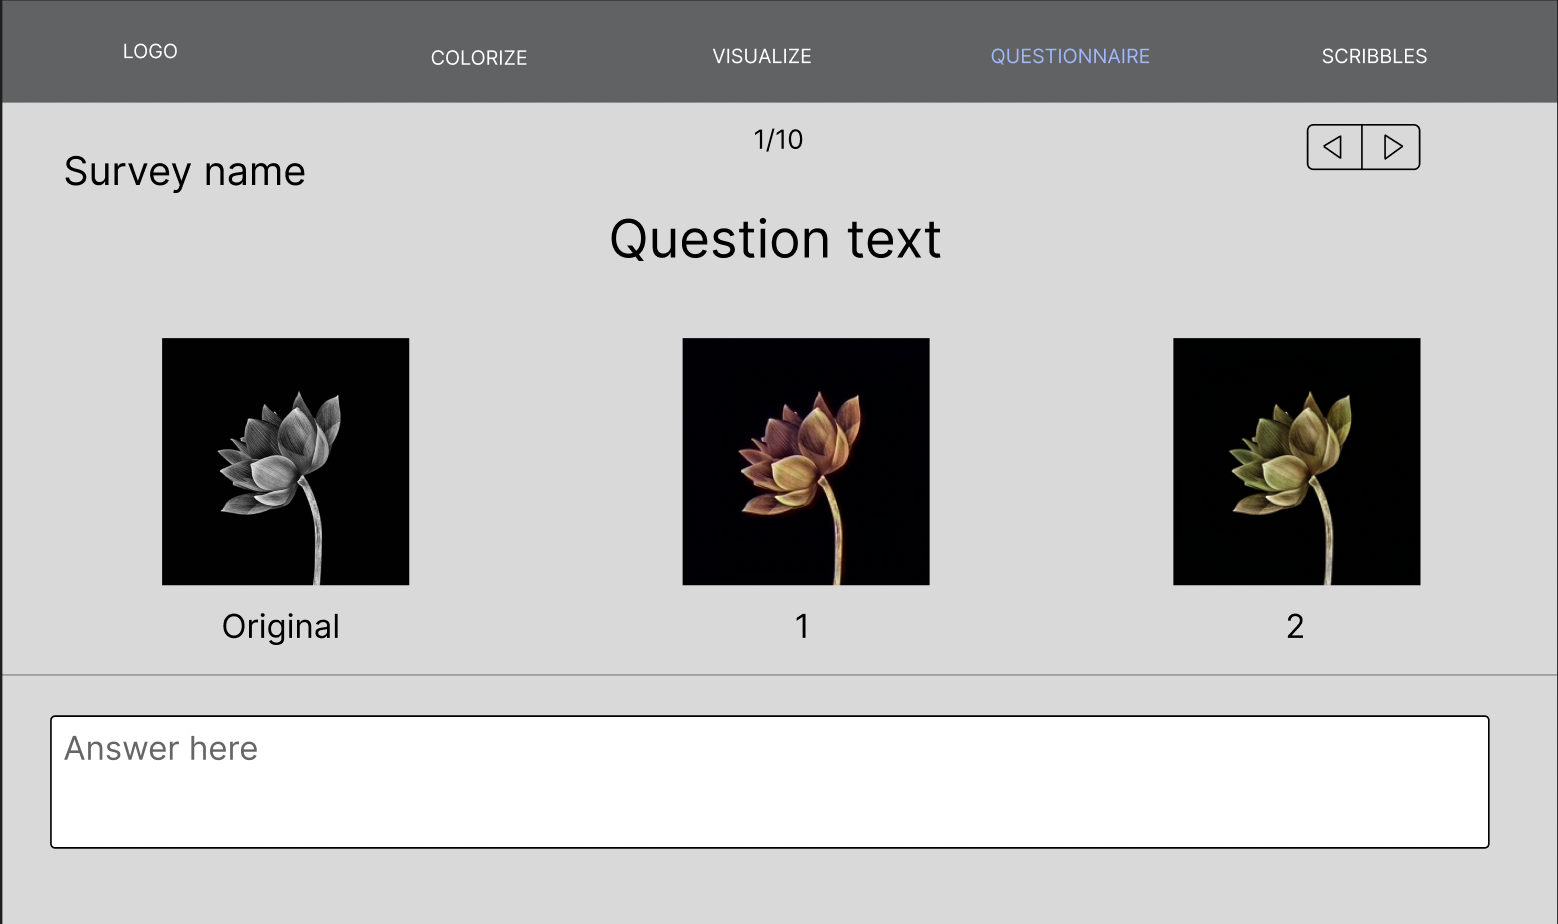
\includegraphics[width=11cm]{questionnaire-repondre.png}
    \caption{Maquette : répondre à un questionnaire}
    \label{fig:maquette-questionnaire-repondre}
\end{figure}

\begin{figure}[htp]
    \centering
    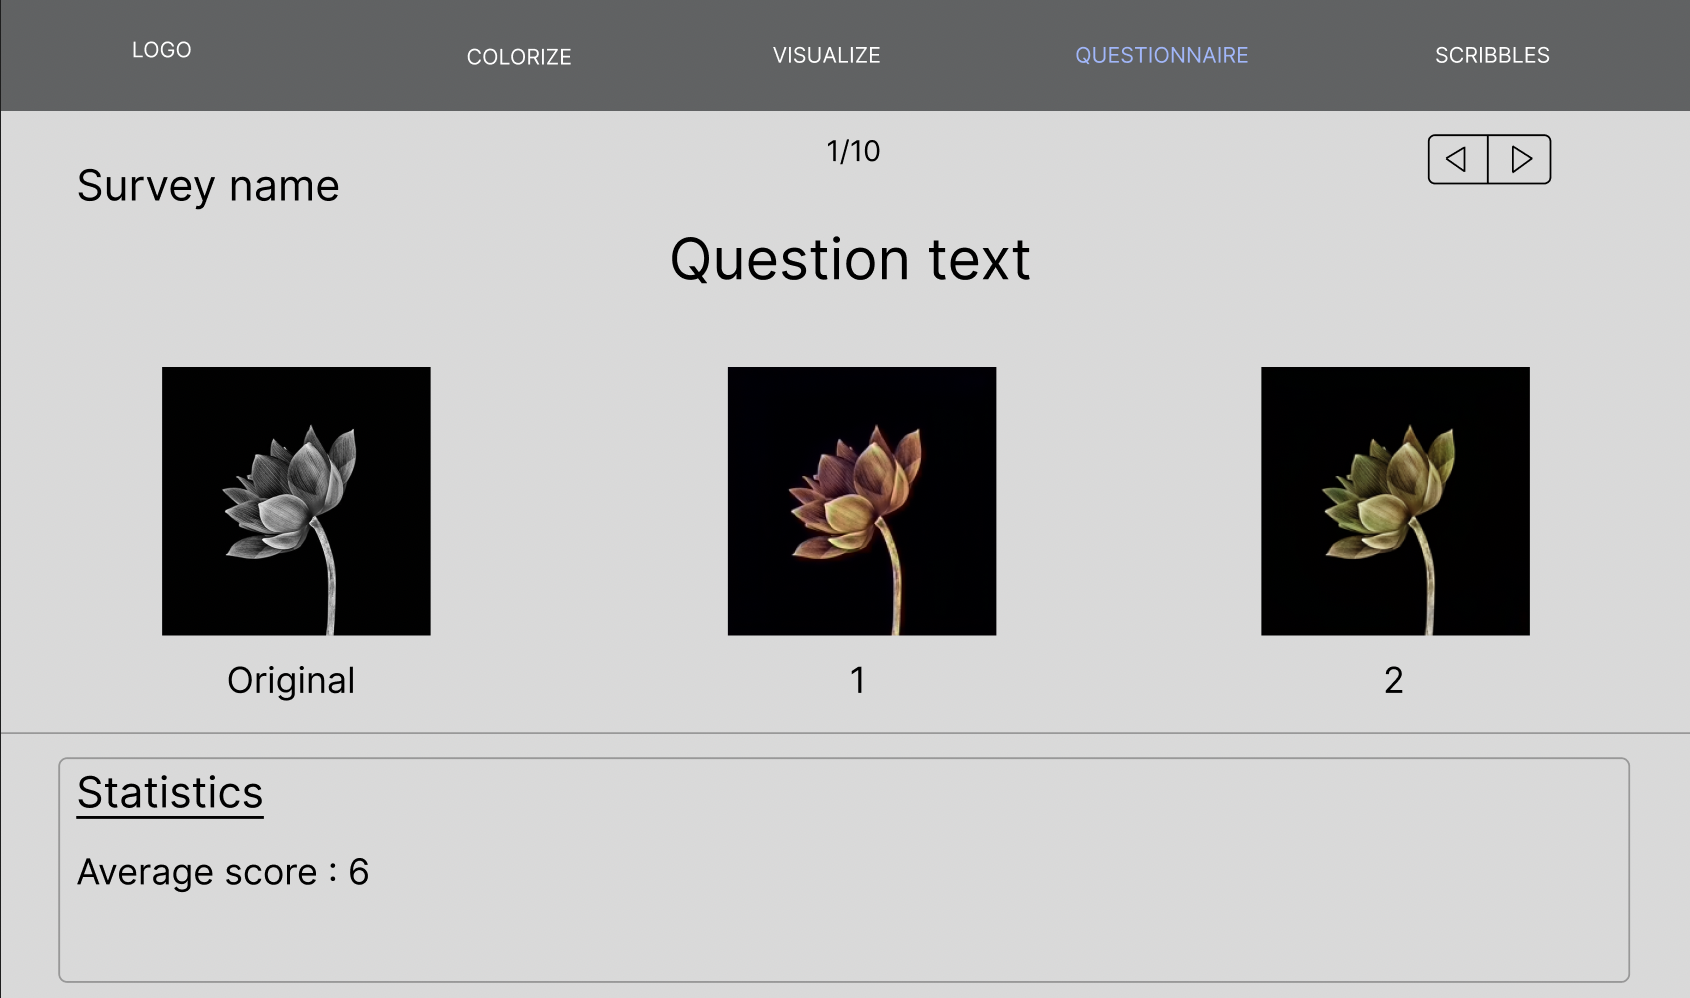
\includegraphics[width=11cm]{questionnaire-visualiser-reponse.png}
    \caption{Maquette : visualiser les réponses à un questionnaire}
    \label{fig:maquette-questionnaire-visualiser-reponse}
\end{figure}

\begin{figure}[htp]
    \centering
    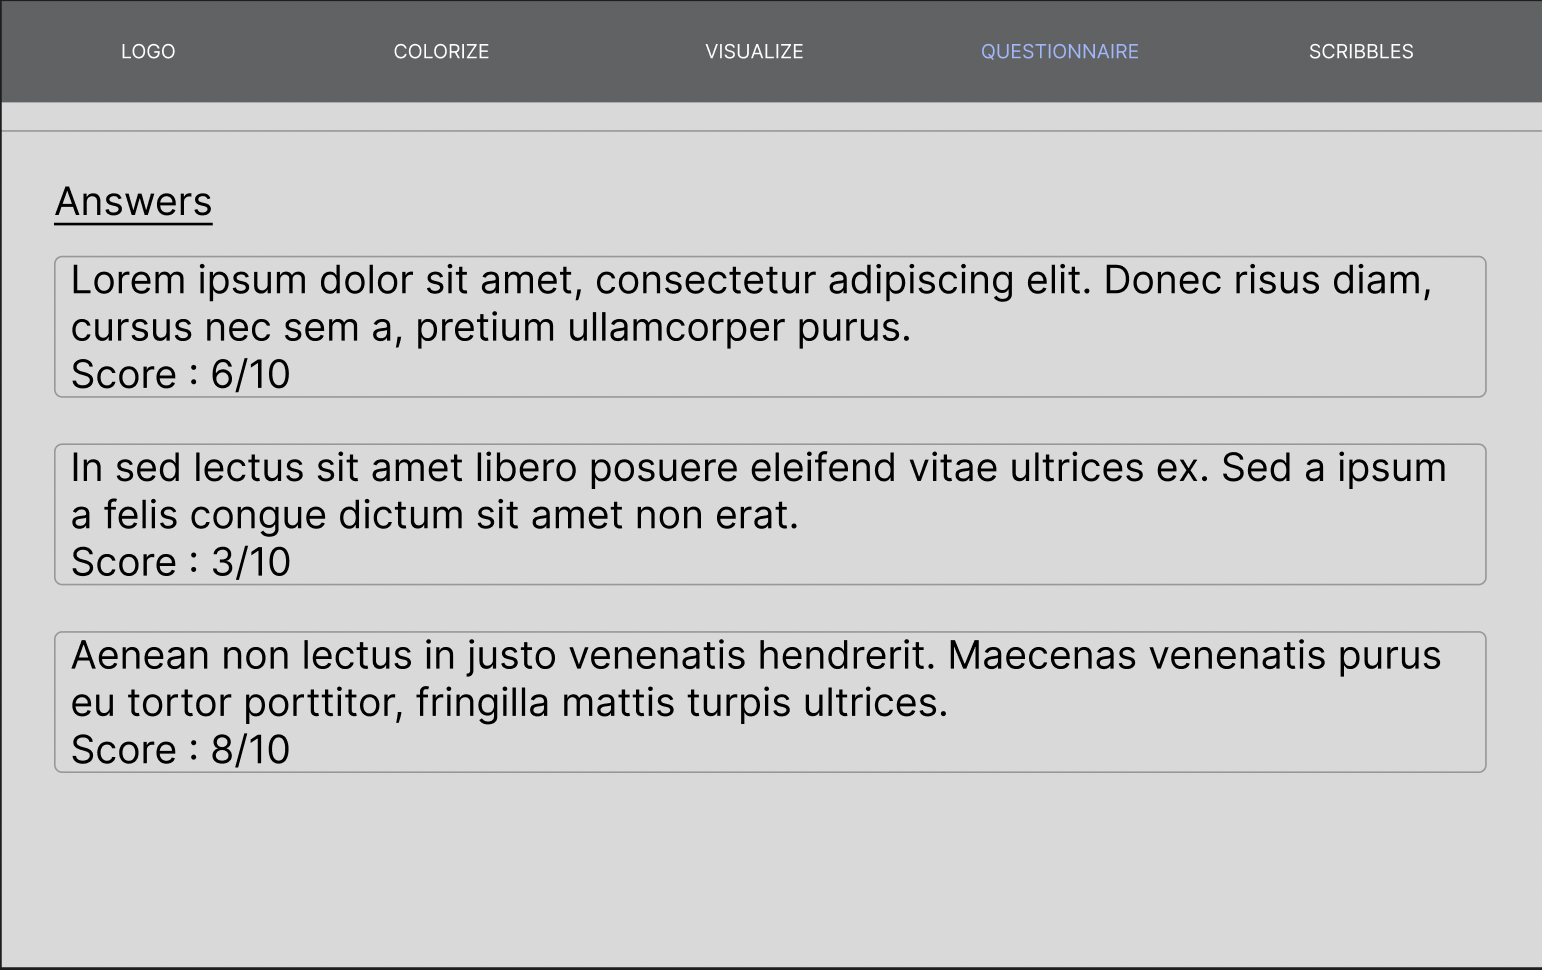
\includegraphics[width=11cm]{questionnaire-visualiser-reponse2.png}
    \caption{Maquette : visualiser les réponses à un questionnaire (bis)}
    \label{fig:maquette-questionnaire-visualiser-reponse2}
\end{figure}

\begin{figure}[htp]
    \centering
    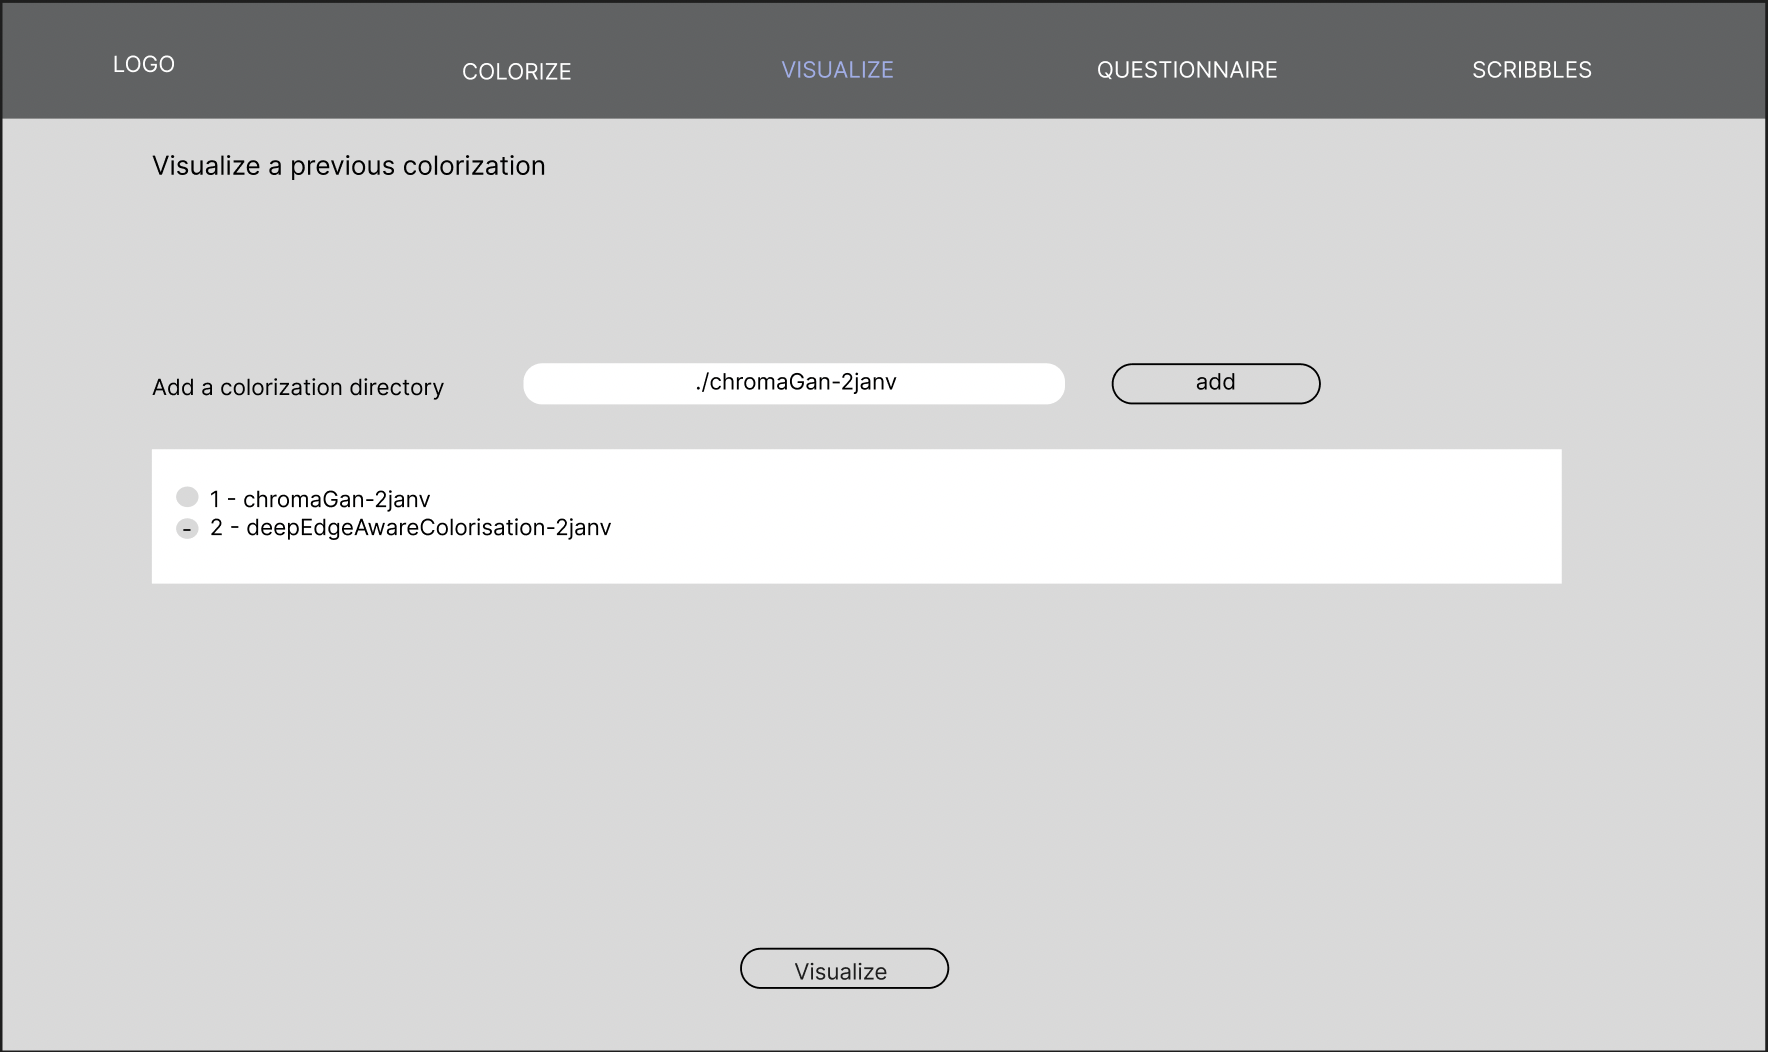
\includegraphics[width=11cm]{visualiser-choix.png}
    \caption{Maquette : paramétrer une visualisation}
    \label{fig:maquette-visualiser-choix}
\end{figure}

\begin{figure}[htp]
    \centering
    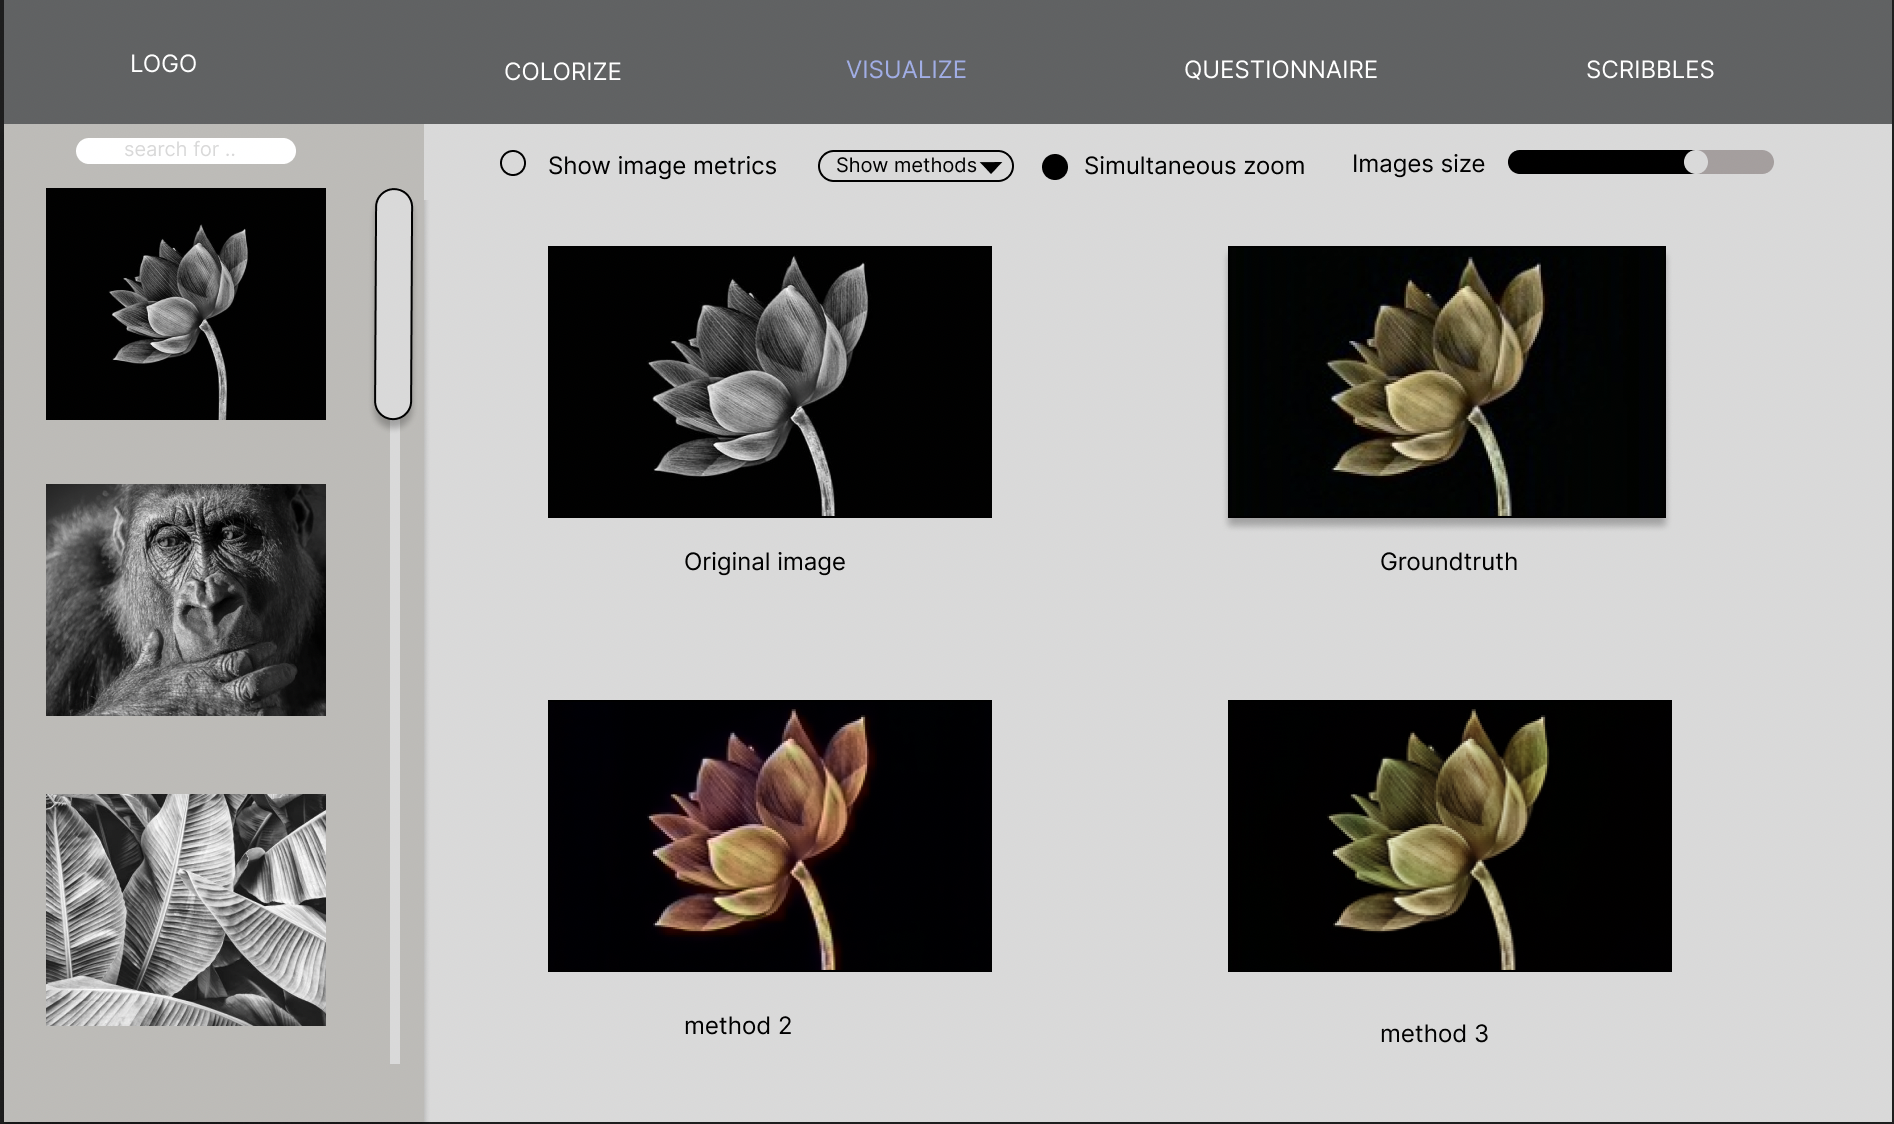
\includegraphics[width=11cm]{visualiser-comparaison1.png}
    \caption{Maquette : visualiser un résultat de colorisation }
    \label{fig:maquette-visualiser-comparaison1}
\end{figure}

\begin{figure}[!ht]
    \centering
    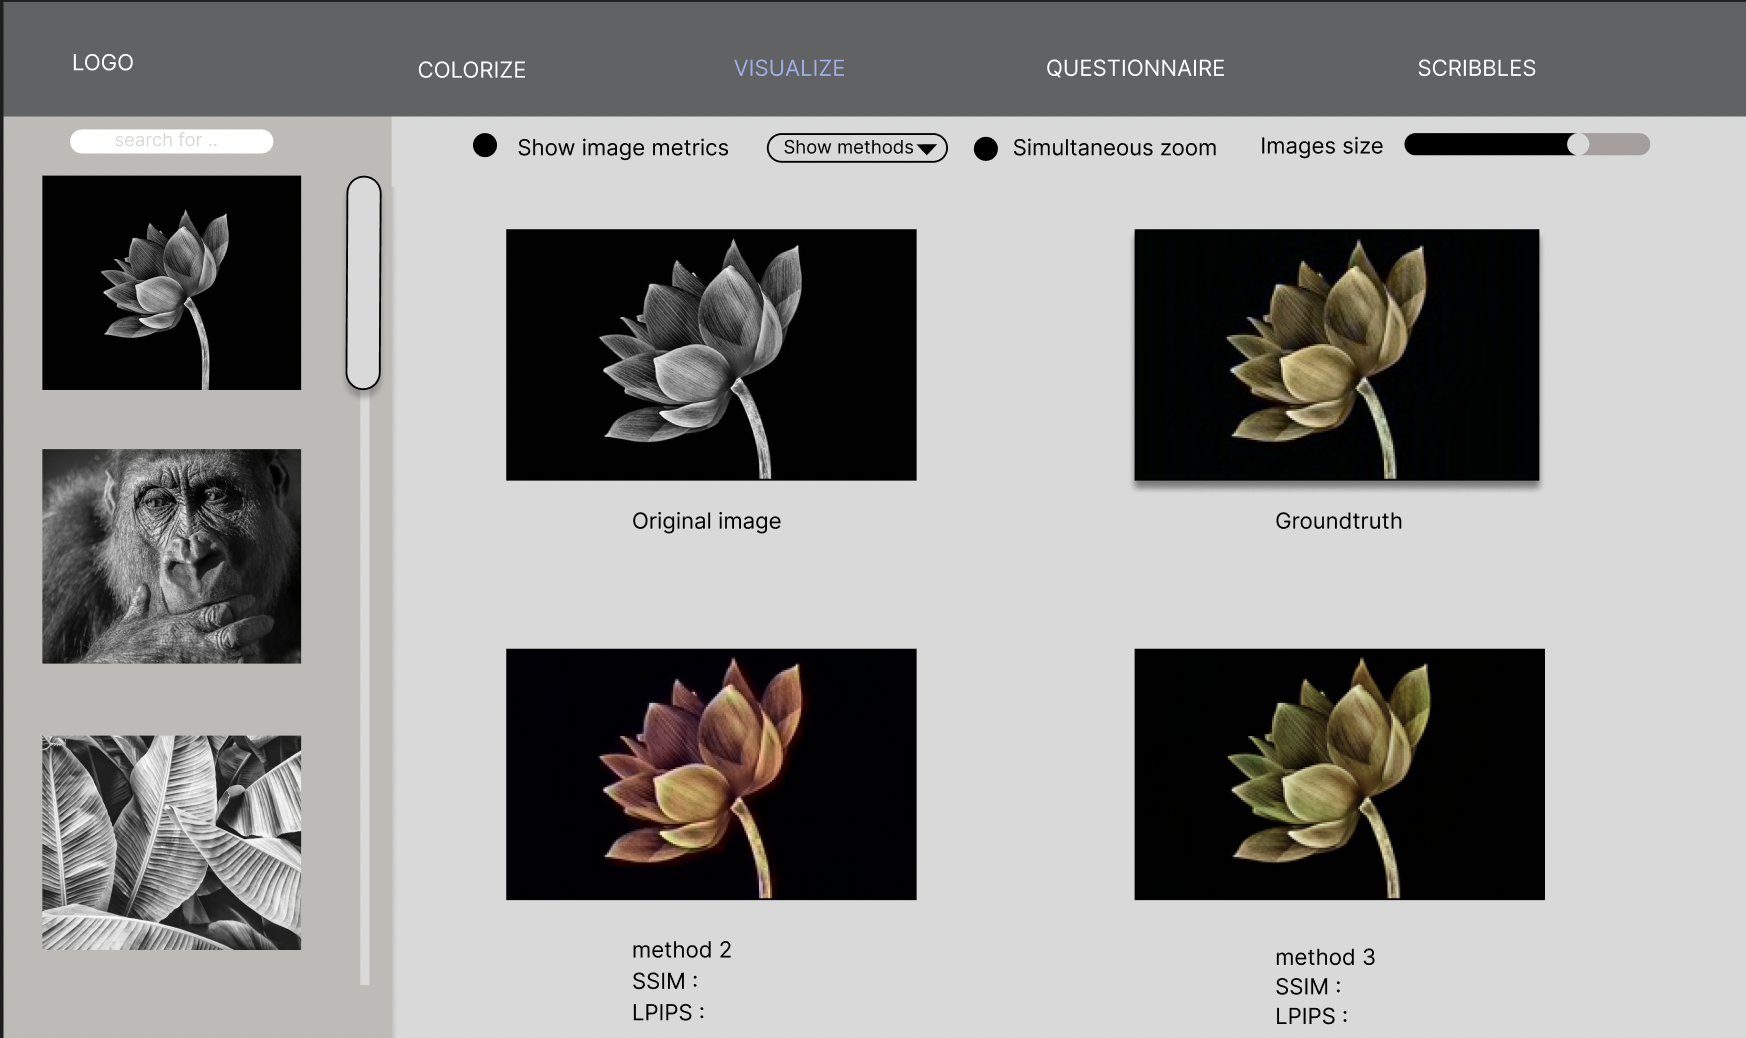
\includegraphics[width=11cm]{visualiser-comparaison2.png}
    \caption{Maquette : visualiser un résultat de colorisation (bis)}
    \label{fig:maquette-visualiser-comparaison2}
\end{figure}

\begin{figure}[!ht]
    \centering
    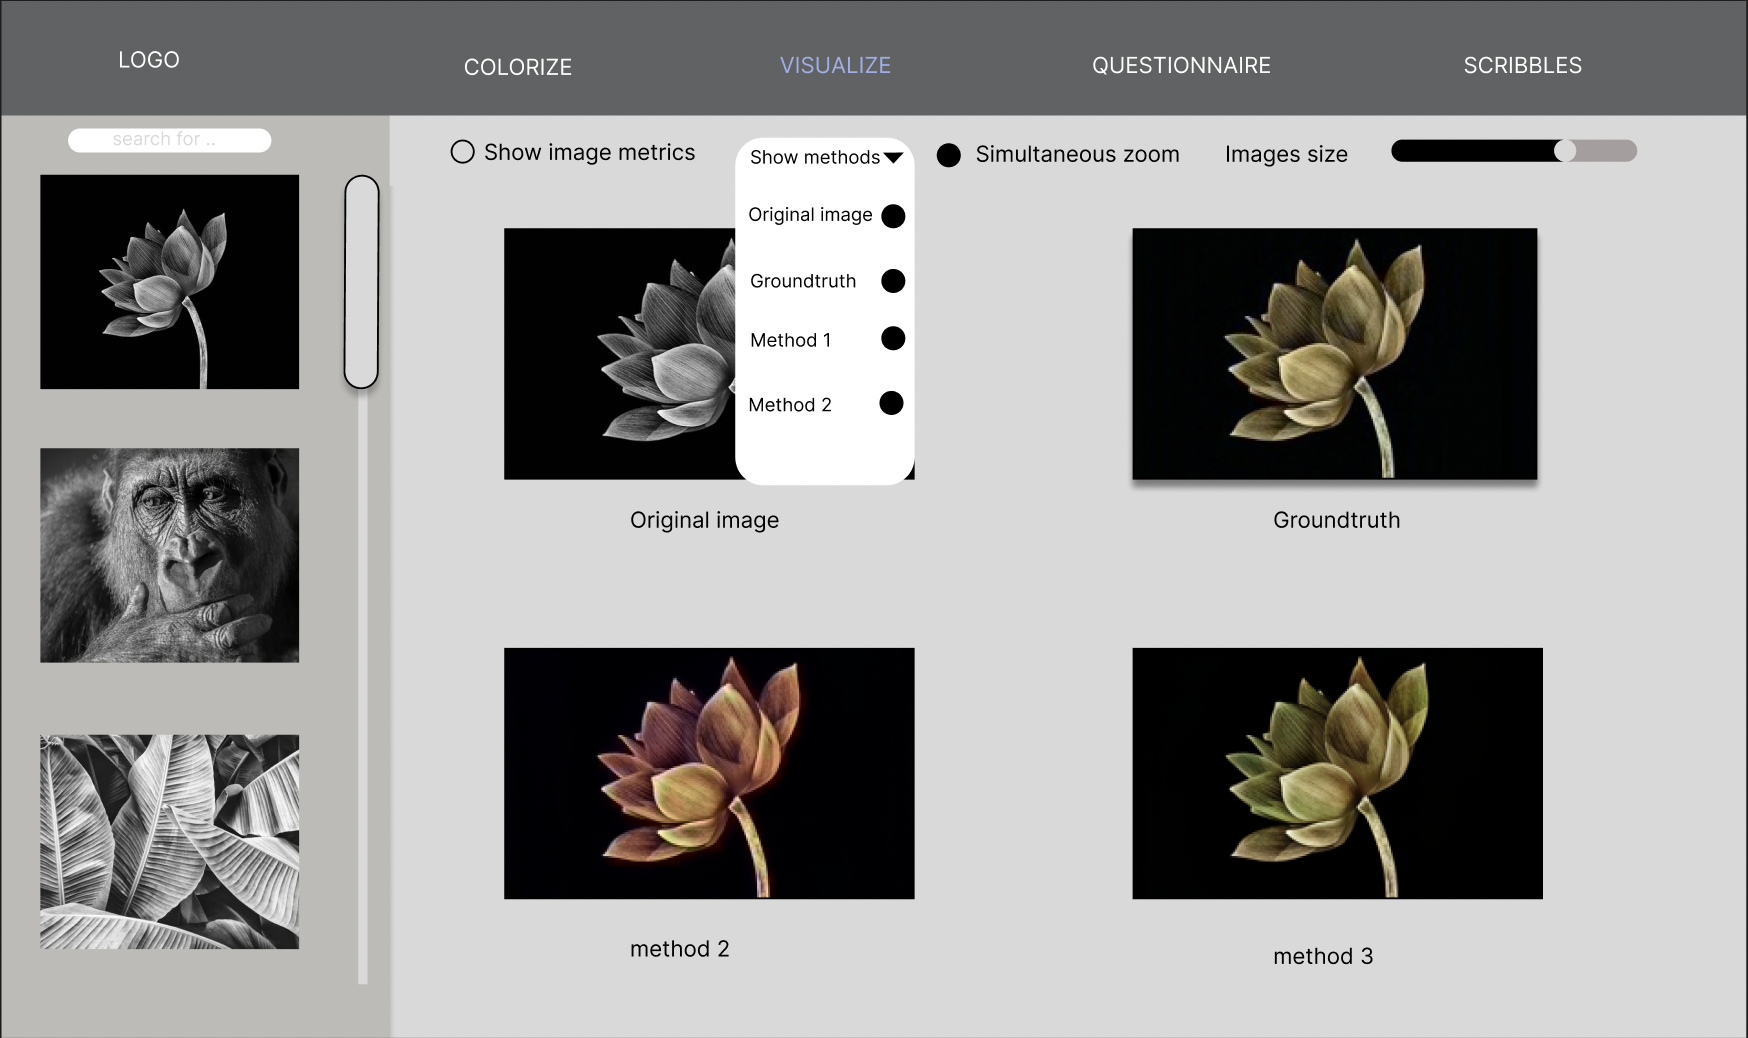
\includegraphics[width=11cm]{visualiser-comparaison3.png}
    \caption{Maquette : visualiser un résultat de colorisation (ter)}
    \label{fig:maquette-visualiser-comparaison3}
\end{figure}

\newpage

\pagebreak

\section{User stories}\label{sec:annexe-user-stories}

\includepdf[pages=-, pagecommand={}]{Temps_taches_V2_-_UserStories_1.pdf}

\section{Use cases}\label{sec:annexe-use-case}

\includepdf[pages=-, pagecommand={}]{Temps_taches_V2_-_UseCase.pdf}

\section{Livrable}\label{sec:annexe-livrable}

\includepdf[pages=-, pagecommand={}]{Temps_taches_V2_-_livrables.pdf}

\pagebreak

\bibliographystyle{plain} 
\bibliography{refs}

\end{document}
